\subsection{L1 -- L2: ván 42}
\label{sec:cs-van-01}
X: \texttt{L1-Random}; O: \texttt{L2-Rule}; khai cuộc 21 (3 nước, đánh dấu $\ast$); 10 nước; kết quả: O (L2) thắng. Cả cặp: L1 thắng 0, hoà 0, thua 100 trên 100 ván; trung vị 10 nước.
\begin{figure}[H]
  \centering
  \begin{subfigure}[t]{.48\linewidth}
    \centering
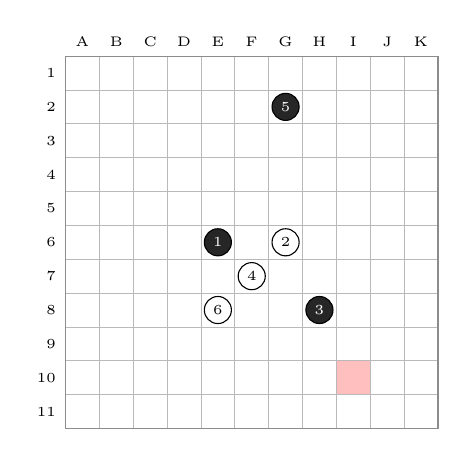
\begin{tikzpicture}[x=0.43cm, y=0.43cm]
\fill[red!25] (8,-9) rectangle (9,-10);
\draw[gray!55, line width=.3pt, step=1] (0,0) grid (11,-11);
\draw[gray!90] (0,0) rectangle (11,-11);
\node[font=\tiny, anchor=south] at (0.5,0) {A};
\node[font=\tiny, anchor=south] at (1.5,0) {B};
\node[font=\tiny, anchor=south] at (2.5,0) {C};
\node[font=\tiny, anchor=south] at (3.5,0) {D};
\node[font=\tiny, anchor=south] at (4.5,0) {E};
\node[font=\tiny, anchor=south] at (5.5,0) {F};
\node[font=\tiny, anchor=south] at (6.5,0) {G};
\node[font=\tiny, anchor=south] at (7.5,0) {H};
\node[font=\tiny, anchor=south] at (8.5,0) {I};
\node[font=\tiny, anchor=south] at (9.5,0) {J};
\node[font=\tiny, anchor=south] at (10.5,0) {K};
\node[font=\tiny, anchor=east] at (0,-0.5) {1};
\node[font=\tiny, anchor=east] at (0,-1.5) {2};
\node[font=\tiny, anchor=east] at (0,-2.5) {3};
\node[font=\tiny, anchor=east] at (0,-3.5) {4};
\node[font=\tiny, anchor=east] at (0,-4.5) {5};
\node[font=\tiny, anchor=east] at (0,-5.5) {6};
\node[font=\tiny, anchor=east] at (0,-6.5) {7};
\node[font=\tiny, anchor=east] at (0,-7.5) {8};
\node[font=\tiny, anchor=east] at (0,-8.5) {9};
\node[font=\tiny, anchor=east] at (0,-9.5) {10};
\node[font=\tiny, anchor=east] at (0,-10.5) {11};
\draw[fill=black!85, line width=.4pt] (6.5,-1.5) circle (.40);
\node[font=\tiny, text=white, inner sep=0pt] at (6.5,-1.5) {5};
\draw[fill=black!85, line width=.4pt] (4.5,-5.5) circle (.40);
\node[font=\tiny, text=white, inner sep=0pt] at (4.5,-5.5) {1};
\draw[fill=white, line width=.4pt] (6.5,-5.5) circle (.40);
\node[font=\tiny, text=black, inner sep=0pt] at (6.5,-5.5) {2};
\draw[fill=white, line width=.4pt] (5.5,-6.5) circle (.40);
\node[font=\tiny, text=black, inner sep=0pt] at (5.5,-6.5) {4};
\draw[fill=white, line width=.4pt] (4.5,-7.5) circle (.40);
\node[font=\tiny, text=black, inner sep=0pt] at (4.5,-7.5) {6};
\draw[fill=black!85, line width=.4pt] (7.5,-7.5) circle (.40);
\node[font=\tiny, text=white, inner sep=0pt] at (7.5,-7.5) {3};
\end{tikzpicture}
    \caption{Trước nước 7 (X đi; ô đỏ là nước đã chọn)}
  \end{subfigure}\hfill
  \begin{subfigure}[t]{.48\linewidth}
    \centering
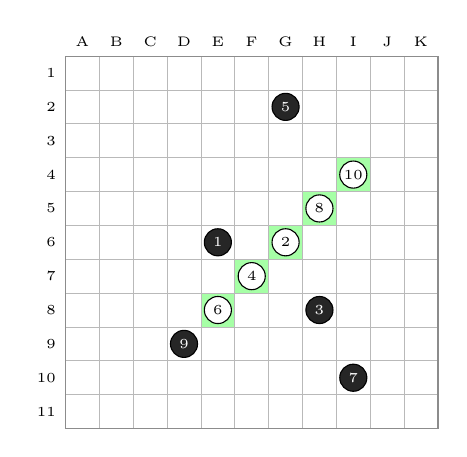
\begin{tikzpicture}[x=0.43cm, y=0.43cm]
\fill[green!35] (8,-3) rectangle (9,-4);
\fill[green!35] (7,-4) rectangle (8,-5);
\fill[green!35] (6,-5) rectangle (7,-6);
\fill[green!35] (5,-6) rectangle (6,-7);
\fill[green!35] (4,-7) rectangle (5,-8);
\draw[gray!55, line width=.3pt, step=1] (0,0) grid (11,-11);
\draw[gray!90] (0,0) rectangle (11,-11);
\node[font=\tiny, anchor=south] at (0.5,0) {A};
\node[font=\tiny, anchor=south] at (1.5,0) {B};
\node[font=\tiny, anchor=south] at (2.5,0) {C};
\node[font=\tiny, anchor=south] at (3.5,0) {D};
\node[font=\tiny, anchor=south] at (4.5,0) {E};
\node[font=\tiny, anchor=south] at (5.5,0) {F};
\node[font=\tiny, anchor=south] at (6.5,0) {G};
\node[font=\tiny, anchor=south] at (7.5,0) {H};
\node[font=\tiny, anchor=south] at (8.5,0) {I};
\node[font=\tiny, anchor=south] at (9.5,0) {J};
\node[font=\tiny, anchor=south] at (10.5,0) {K};
\node[font=\tiny, anchor=east] at (0,-0.5) {1};
\node[font=\tiny, anchor=east] at (0,-1.5) {2};
\node[font=\tiny, anchor=east] at (0,-2.5) {3};
\node[font=\tiny, anchor=east] at (0,-3.5) {4};
\node[font=\tiny, anchor=east] at (0,-4.5) {5};
\node[font=\tiny, anchor=east] at (0,-5.5) {6};
\node[font=\tiny, anchor=east] at (0,-6.5) {7};
\node[font=\tiny, anchor=east] at (0,-7.5) {8};
\node[font=\tiny, anchor=east] at (0,-8.5) {9};
\node[font=\tiny, anchor=east] at (0,-9.5) {10};
\node[font=\tiny, anchor=east] at (0,-10.5) {11};
\draw[fill=black!85, line width=.4pt] (6.5,-1.5) circle (.40);
\node[font=\tiny, text=white, inner sep=0pt] at (6.5,-1.5) {5};
\draw[fill=white, line width=.4pt] (8.5,-3.5) circle (.40);
\node[font=\tiny, text=black, inner sep=0pt] at (8.5,-3.5) {10};
\draw[fill=white, line width=.4pt] (7.5,-4.5) circle (.40);
\node[font=\tiny, text=black, inner sep=0pt] at (7.5,-4.5) {8};
\draw[fill=black!85, line width=.4pt] (4.5,-5.5) circle (.40);
\node[font=\tiny, text=white, inner sep=0pt] at (4.5,-5.5) {1};
\draw[fill=white, line width=.4pt] (6.5,-5.5) circle (.40);
\node[font=\tiny, text=black, inner sep=0pt] at (6.5,-5.5) {2};
\draw[fill=white, line width=.4pt] (5.5,-6.5) circle (.40);
\node[font=\tiny, text=black, inner sep=0pt] at (5.5,-6.5) {4};
\draw[fill=white, line width=.4pt] (4.5,-7.5) circle (.40);
\node[font=\tiny, text=black, inner sep=0pt] at (4.5,-7.5) {6};
\draw[fill=black!85, line width=.4pt] (7.5,-7.5) circle (.40);
\node[font=\tiny, text=white, inner sep=0pt] at (7.5,-7.5) {3};
\draw[fill=black!85, line width=.4pt] (3.5,-8.5) circle (.40);
\node[font=\tiny, text=white, inner sep=0pt] at (3.5,-8.5) {9};
\draw[fill=black!85, line width=.4pt] (8.5,-9.5) circle (.40);
\node[font=\tiny, text=white, inner sep=0pt] at (8.5,-9.5) {7};
\end{tikzpicture}
    \caption{Thế cuối (ô xanh: dãy thắng)}
  \end{subfigure}
  \caption{Ván 42 (L1 cầm X, L2 cầm O).}
  \label{fig:cs-van-01}
\end{figure}
{\footnotesize\linespread{1}\selectfont
\noindent\begin{tabularx}{\linewidth}{*{6}{X}}
\toprule
1.~X E6$^\ast$ & 3.~X H8$^\ast$ & 5.~X G2 & 7.~X I10 & 9.~X D9 &  \\
2.~O G6$^\ast$ & 4.~O F7 & 6.~O E8 & 8.~O H5 & 10.~O I4 &  \\
\bottomrule
\end{tabularx}\par}
\paragraph{Diễn biến chiến thuật.}
\begin{itemize}\small
\setlength{\itemsep}{0pt}
  \item Nước 7 (X=L1, I10): để đối thủ có VCF: H5--I4--D9.
  \item Nước 8 (O=L2, H5): đang có VCF 2 nước và đi đúng một đường (H5--I4--D9 là đường ngắn nhất).
  \item Nước 9 (X=L1, D9): đối thủ đang có các ô thắng I4, D9, không đỡ hết được.
  \item Nước 10 (O=L2, I4): thắng ngay.
\end{itemize}
Thời gian trung vị mỗi nước: X 0,0 ms, O 1,1 ms.
\clearpage

\subsection{L1 -- L3: ván 125}
\label{sec:cs-van-02}
X: \texttt{L3-AlphaBeta}; O: \texttt{L1-Random}; khai cuộc 12 (4 nước, đánh dấu $\ast$); 11 nước; kết quả: X (L3) thắng. Cả cặp: L1 thắng 0, hoà 0, thua 100 trên 100 ván; trung vị 11 nước.
\begin{figure}[H]
  \centering
  \begin{subfigure}[t]{.48\linewidth}
    \centering
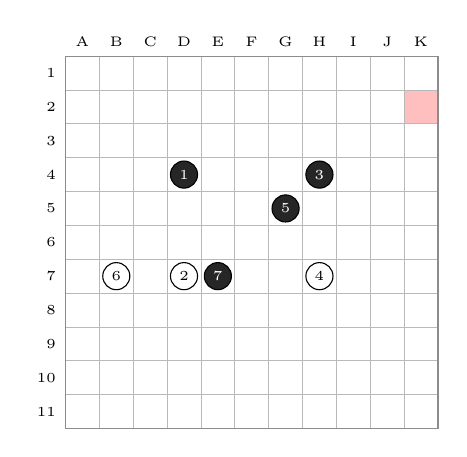
\begin{tikzpicture}[x=0.43cm, y=0.43cm]
\fill[red!25] (10,-1) rectangle (11,-2);
\draw[gray!55, line width=.3pt, step=1] (0,0) grid (11,-11);
\draw[gray!90] (0,0) rectangle (11,-11);
\node[font=\tiny, anchor=south] at (0.5,0) {A};
\node[font=\tiny, anchor=south] at (1.5,0) {B};
\node[font=\tiny, anchor=south] at (2.5,0) {C};
\node[font=\tiny, anchor=south] at (3.5,0) {D};
\node[font=\tiny, anchor=south] at (4.5,0) {E};
\node[font=\tiny, anchor=south] at (5.5,0) {F};
\node[font=\tiny, anchor=south] at (6.5,0) {G};
\node[font=\tiny, anchor=south] at (7.5,0) {H};
\node[font=\tiny, anchor=south] at (8.5,0) {I};
\node[font=\tiny, anchor=south] at (9.5,0) {J};
\node[font=\tiny, anchor=south] at (10.5,0) {K};
\node[font=\tiny, anchor=east] at (0,-0.5) {1};
\node[font=\tiny, anchor=east] at (0,-1.5) {2};
\node[font=\tiny, anchor=east] at (0,-2.5) {3};
\node[font=\tiny, anchor=east] at (0,-3.5) {4};
\node[font=\tiny, anchor=east] at (0,-4.5) {5};
\node[font=\tiny, anchor=east] at (0,-5.5) {6};
\node[font=\tiny, anchor=east] at (0,-6.5) {7};
\node[font=\tiny, anchor=east] at (0,-7.5) {8};
\node[font=\tiny, anchor=east] at (0,-8.5) {9};
\node[font=\tiny, anchor=east] at (0,-9.5) {10};
\node[font=\tiny, anchor=east] at (0,-10.5) {11};
\draw[fill=black!85, line width=.4pt] (3.5,-3.5) circle (.40);
\node[font=\tiny, text=white, inner sep=0pt] at (3.5,-3.5) {1};
\draw[fill=black!85, line width=.4pt] (7.5,-3.5) circle (.40);
\node[font=\tiny, text=white, inner sep=0pt] at (7.5,-3.5) {3};
\draw[fill=black!85, line width=.4pt] (6.5,-4.5) circle (.40);
\node[font=\tiny, text=white, inner sep=0pt] at (6.5,-4.5) {5};
\draw[fill=white, line width=.4pt] (1.5,-6.5) circle (.40);
\node[font=\tiny, text=black, inner sep=0pt] at (1.5,-6.5) {6};
\draw[fill=white, line width=.4pt] (3.5,-6.5) circle (.40);
\node[font=\tiny, text=black, inner sep=0pt] at (3.5,-6.5) {2};
\draw[fill=black!85, line width=.4pt] (4.5,-6.5) circle (.40);
\node[font=\tiny, text=white, inner sep=0pt] at (4.5,-6.5) {7};
\draw[fill=white, line width=.4pt] (7.5,-6.5) circle (.40);
\node[font=\tiny, text=black, inner sep=0pt] at (7.5,-6.5) {4};
\end{tikzpicture}
    \caption{Trước nước 8 (O đi; ô đỏ là nước đã chọn)}
  \end{subfigure}\hfill
  \begin{subfigure}[t]{.48\linewidth}
    \centering
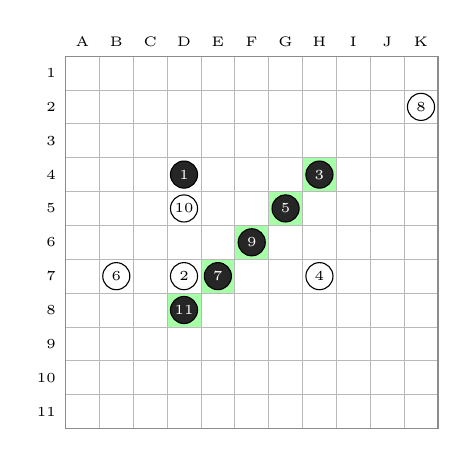
\begin{tikzpicture}[x=0.43cm, y=0.43cm]
\fill[green!35] (3,-7) rectangle (4,-8);
\fill[green!35] (4,-6) rectangle (5,-7);
\fill[green!35] (5,-5) rectangle (6,-6);
\fill[green!35] (6,-4) rectangle (7,-5);
\fill[green!35] (7,-3) rectangle (8,-4);
\draw[gray!55, line width=.3pt, step=1] (0,0) grid (11,-11);
\draw[gray!90] (0,0) rectangle (11,-11);
\node[font=\tiny, anchor=south] at (0.5,0) {A};
\node[font=\tiny, anchor=south] at (1.5,0) {B};
\node[font=\tiny, anchor=south] at (2.5,0) {C};
\node[font=\tiny, anchor=south] at (3.5,0) {D};
\node[font=\tiny, anchor=south] at (4.5,0) {E};
\node[font=\tiny, anchor=south] at (5.5,0) {F};
\node[font=\tiny, anchor=south] at (6.5,0) {G};
\node[font=\tiny, anchor=south] at (7.5,0) {H};
\node[font=\tiny, anchor=south] at (8.5,0) {I};
\node[font=\tiny, anchor=south] at (9.5,0) {J};
\node[font=\tiny, anchor=south] at (10.5,0) {K};
\node[font=\tiny, anchor=east] at (0,-0.5) {1};
\node[font=\tiny, anchor=east] at (0,-1.5) {2};
\node[font=\tiny, anchor=east] at (0,-2.5) {3};
\node[font=\tiny, anchor=east] at (0,-3.5) {4};
\node[font=\tiny, anchor=east] at (0,-4.5) {5};
\node[font=\tiny, anchor=east] at (0,-5.5) {6};
\node[font=\tiny, anchor=east] at (0,-6.5) {7};
\node[font=\tiny, anchor=east] at (0,-7.5) {8};
\node[font=\tiny, anchor=east] at (0,-8.5) {9};
\node[font=\tiny, anchor=east] at (0,-9.5) {10};
\node[font=\tiny, anchor=east] at (0,-10.5) {11};
\draw[fill=white, line width=.4pt] (10.5,-1.5) circle (.40);
\node[font=\tiny, text=black, inner sep=0pt] at (10.5,-1.5) {8};
\draw[fill=black!85, line width=.4pt] (3.5,-3.5) circle (.40);
\node[font=\tiny, text=white, inner sep=0pt] at (3.5,-3.5) {1};
\draw[fill=black!85, line width=.4pt] (7.5,-3.5) circle (.40);
\node[font=\tiny, text=white, inner sep=0pt] at (7.5,-3.5) {3};
\draw[fill=white, line width=.4pt] (3.5,-4.5) circle (.40);
\node[font=\tiny, text=black, inner sep=0pt] at (3.5,-4.5) {10};
\draw[fill=black!85, line width=.4pt] (6.5,-4.5) circle (.40);
\node[font=\tiny, text=white, inner sep=0pt] at (6.5,-4.5) {5};
\draw[fill=black!85, line width=.4pt] (5.5,-5.5) circle (.40);
\node[font=\tiny, text=white, inner sep=0pt] at (5.5,-5.5) {9};
\draw[fill=white, line width=.4pt] (1.5,-6.5) circle (.40);
\node[font=\tiny, text=black, inner sep=0pt] at (1.5,-6.5) {6};
\draw[fill=white, line width=.4pt] (3.5,-6.5) circle (.40);
\node[font=\tiny, text=black, inner sep=0pt] at (3.5,-6.5) {2};
\draw[fill=black!85, line width=.4pt] (4.5,-6.5) circle (.40);
\node[font=\tiny, text=white, inner sep=0pt] at (4.5,-6.5) {7};
\draw[fill=white, line width=.4pt] (7.5,-6.5) circle (.40);
\node[font=\tiny, text=black, inner sep=0pt] at (7.5,-6.5) {4};
\draw[fill=black!85, line width=.4pt] (3.5,-7.5) circle (.40);
\node[font=\tiny, text=white, inner sep=0pt] at (3.5,-7.5) {11};
\end{tikzpicture}
    \caption{Thế cuối (ô xanh: dãy thắng)}
  \end{subfigure}
  \caption{Ván 125 (L3 cầm X, L1 cầm O).}
  \label{fig:cs-van-02}
\end{figure}
{\footnotesize\linespread{1}\selectfont
\noindent\begin{tabularx}{\linewidth}{*{6}{X}}
\toprule
1.~X D4$^\ast$ & 3.~X H4$^\ast$ & 5.~X G5 & 7.~X E7 & 9.~X F6 & 11.~X D8 \\
2.~O D7$^\ast$ & 4.~O H7$^\ast$ & 6.~O B7 & 8.~O K2 & 10.~O D5 &  \\
\bottomrule
\end{tabularx}\par}
\paragraph{Diễn biến chiến thuật.}
\begin{itemize}\small
\setlength{\itemsep}{0pt}
  \item Nước 8 (O=L1, K2): để đối thủ có VCF: F6--I3--D8.
  \item Nước 9 (X=L3, F6): đang có VCF 2 nước và đi đúng một đường (F6--I3--D8 là đường ngắn nhất).
  \item Nước 10 (O=L1, D5): đối thủ đang có các ô thắng I3, D8, không đỡ hết được.
  \item Nước 11 (X=L3, D8): thắng ngay.
\end{itemize}
Thời gian trung vị mỗi nước: X 15,8 ms, O 0,0 ms.
\clearpage

\subsection{L1 -- L4: ván 293}
\label{sec:cs-van-03}
X: \texttt{L4-MCTS}; O: \texttt{L1-Random}; khai cuộc 46 (3 nước, đánh dấu $\ast$); 31 nước; kết quả: X (L4) thắng. Cả cặp: L1 thắng 1, hoà 0, thua 99 trên 100 ván; trung vị 32 nước.
\begin{figure}[H]
  \centering
  \begin{subfigure}[t]{.48\linewidth}
    \centering
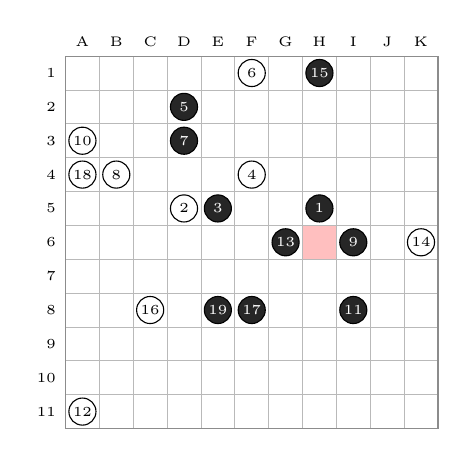
\begin{tikzpicture}[x=0.43cm, y=0.43cm]
\fill[red!25] (7,-5) rectangle (8,-6);
\draw[gray!55, line width=.3pt, step=1] (0,0) grid (11,-11);
\draw[gray!90] (0,0) rectangle (11,-11);
\node[font=\tiny, anchor=south] at (0.5,0) {A};
\node[font=\tiny, anchor=south] at (1.5,0) {B};
\node[font=\tiny, anchor=south] at (2.5,0) {C};
\node[font=\tiny, anchor=south] at (3.5,0) {D};
\node[font=\tiny, anchor=south] at (4.5,0) {E};
\node[font=\tiny, anchor=south] at (5.5,0) {F};
\node[font=\tiny, anchor=south] at (6.5,0) {G};
\node[font=\tiny, anchor=south] at (7.5,0) {H};
\node[font=\tiny, anchor=south] at (8.5,0) {I};
\node[font=\tiny, anchor=south] at (9.5,0) {J};
\node[font=\tiny, anchor=south] at (10.5,0) {K};
\node[font=\tiny, anchor=east] at (0,-0.5) {1};
\node[font=\tiny, anchor=east] at (0,-1.5) {2};
\node[font=\tiny, anchor=east] at (0,-2.5) {3};
\node[font=\tiny, anchor=east] at (0,-3.5) {4};
\node[font=\tiny, anchor=east] at (0,-4.5) {5};
\node[font=\tiny, anchor=east] at (0,-5.5) {6};
\node[font=\tiny, anchor=east] at (0,-6.5) {7};
\node[font=\tiny, anchor=east] at (0,-7.5) {8};
\node[font=\tiny, anchor=east] at (0,-8.5) {9};
\node[font=\tiny, anchor=east] at (0,-9.5) {10};
\node[font=\tiny, anchor=east] at (0,-10.5) {11};
\draw[fill=white, line width=.4pt] (5.5,-0.5) circle (.40);
\node[font=\tiny, text=black, inner sep=0pt] at (5.5,-0.5) {6};
\draw[fill=black!85, line width=.4pt] (7.5,-0.5) circle (.40);
\node[font=\tiny, text=white, inner sep=0pt] at (7.5,-0.5) {15};
\draw[fill=black!85, line width=.4pt] (3.5,-1.5) circle (.40);
\node[font=\tiny, text=white, inner sep=0pt] at (3.5,-1.5) {5};
\draw[fill=white, line width=.4pt] (0.5,-2.5) circle (.40);
\node[font=\tiny, text=black, inner sep=0pt] at (0.5,-2.5) {10};
\draw[fill=black!85, line width=.4pt] (3.5,-2.5) circle (.40);
\node[font=\tiny, text=white, inner sep=0pt] at (3.5,-2.5) {7};
\draw[fill=white, line width=.4pt] (0.5,-3.5) circle (.40);
\node[font=\tiny, text=black, inner sep=0pt] at (0.5,-3.5) {18};
\draw[fill=white, line width=.4pt] (1.5,-3.5) circle (.40);
\node[font=\tiny, text=black, inner sep=0pt] at (1.5,-3.5) {8};
\draw[fill=white, line width=.4pt] (5.5,-3.5) circle (.40);
\node[font=\tiny, text=black, inner sep=0pt] at (5.5,-3.5) {4};
\draw[fill=white, line width=.4pt] (3.5,-4.5) circle (.40);
\node[font=\tiny, text=black, inner sep=0pt] at (3.5,-4.5) {2};
\draw[fill=black!85, line width=.4pt] (4.5,-4.5) circle (.40);
\node[font=\tiny, text=white, inner sep=0pt] at (4.5,-4.5) {3};
\draw[fill=black!85, line width=.4pt] (7.5,-4.5) circle (.40);
\node[font=\tiny, text=white, inner sep=0pt] at (7.5,-4.5) {1};
\draw[fill=black!85, line width=.4pt] (6.5,-5.5) circle (.40);
\node[font=\tiny, text=white, inner sep=0pt] at (6.5,-5.5) {13};
\draw[fill=black!85, line width=.4pt] (8.5,-5.5) circle (.40);
\node[font=\tiny, text=white, inner sep=0pt] at (8.5,-5.5) {9};
\draw[fill=white, line width=.4pt] (10.5,-5.5) circle (.40);
\node[font=\tiny, text=black, inner sep=0pt] at (10.5,-5.5) {14};
\draw[fill=white, line width=.4pt] (2.5,-7.5) circle (.40);
\node[font=\tiny, text=black, inner sep=0pt] at (2.5,-7.5) {16};
\draw[fill=black!85, line width=.4pt] (4.5,-7.5) circle (.40);
\node[font=\tiny, text=white, inner sep=0pt] at (4.5,-7.5) {19};
\draw[fill=black!85, line width=.4pt] (5.5,-7.5) circle (.40);
\node[font=\tiny, text=white, inner sep=0pt] at (5.5,-7.5) {17};
\draw[fill=black!85, line width=.4pt] (8.5,-7.5) circle (.40);
\node[font=\tiny, text=white, inner sep=0pt] at (8.5,-7.5) {11};
\draw[fill=white, line width=.4pt] (0.5,-10.5) circle (.40);
\node[font=\tiny, text=black, inner sep=0pt] at (0.5,-10.5) {12};
\end{tikzpicture}
    \caption{Trước nước 20 (O đi; ô đỏ là nước đã chọn)}
  \end{subfigure}\hfill
  \begin{subfigure}[t]{.48\linewidth}
    \centering
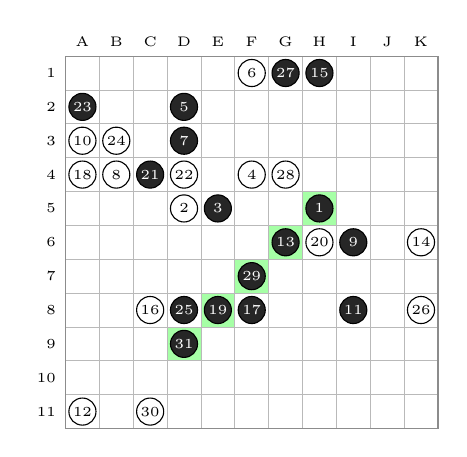
\begin{tikzpicture}[x=0.43cm, y=0.43cm]
\fill[green!35] (3,-8) rectangle (4,-9);
\fill[green!35] (4,-7) rectangle (5,-8);
\fill[green!35] (5,-6) rectangle (6,-7);
\fill[green!35] (6,-5) rectangle (7,-6);
\fill[green!35] (7,-4) rectangle (8,-5);
\draw[gray!55, line width=.3pt, step=1] (0,0) grid (11,-11);
\draw[gray!90] (0,0) rectangle (11,-11);
\node[font=\tiny, anchor=south] at (0.5,0) {A};
\node[font=\tiny, anchor=south] at (1.5,0) {B};
\node[font=\tiny, anchor=south] at (2.5,0) {C};
\node[font=\tiny, anchor=south] at (3.5,0) {D};
\node[font=\tiny, anchor=south] at (4.5,0) {E};
\node[font=\tiny, anchor=south] at (5.5,0) {F};
\node[font=\tiny, anchor=south] at (6.5,0) {G};
\node[font=\tiny, anchor=south] at (7.5,0) {H};
\node[font=\tiny, anchor=south] at (8.5,0) {I};
\node[font=\tiny, anchor=south] at (9.5,0) {J};
\node[font=\tiny, anchor=south] at (10.5,0) {K};
\node[font=\tiny, anchor=east] at (0,-0.5) {1};
\node[font=\tiny, anchor=east] at (0,-1.5) {2};
\node[font=\tiny, anchor=east] at (0,-2.5) {3};
\node[font=\tiny, anchor=east] at (0,-3.5) {4};
\node[font=\tiny, anchor=east] at (0,-4.5) {5};
\node[font=\tiny, anchor=east] at (0,-5.5) {6};
\node[font=\tiny, anchor=east] at (0,-6.5) {7};
\node[font=\tiny, anchor=east] at (0,-7.5) {8};
\node[font=\tiny, anchor=east] at (0,-8.5) {9};
\node[font=\tiny, anchor=east] at (0,-9.5) {10};
\node[font=\tiny, anchor=east] at (0,-10.5) {11};
\draw[fill=white, line width=.4pt] (5.5,-0.5) circle (.40);
\node[font=\tiny, text=black, inner sep=0pt] at (5.5,-0.5) {6};
\draw[fill=black!85, line width=.4pt] (6.5,-0.5) circle (.40);
\node[font=\tiny, text=white, inner sep=0pt] at (6.5,-0.5) {27};
\draw[fill=black!85, line width=.4pt] (7.5,-0.5) circle (.40);
\node[font=\tiny, text=white, inner sep=0pt] at (7.5,-0.5) {15};
\draw[fill=black!85, line width=.4pt] (0.5,-1.5) circle (.40);
\node[font=\tiny, text=white, inner sep=0pt] at (0.5,-1.5) {23};
\draw[fill=black!85, line width=.4pt] (3.5,-1.5) circle (.40);
\node[font=\tiny, text=white, inner sep=0pt] at (3.5,-1.5) {5};
\draw[fill=white, line width=.4pt] (0.5,-2.5) circle (.40);
\node[font=\tiny, text=black, inner sep=0pt] at (0.5,-2.5) {10};
\draw[fill=white, line width=.4pt] (1.5,-2.5) circle (.40);
\node[font=\tiny, text=black, inner sep=0pt] at (1.5,-2.5) {24};
\draw[fill=black!85, line width=.4pt] (3.5,-2.5) circle (.40);
\node[font=\tiny, text=white, inner sep=0pt] at (3.5,-2.5) {7};
\draw[fill=white, line width=.4pt] (0.5,-3.5) circle (.40);
\node[font=\tiny, text=black, inner sep=0pt] at (0.5,-3.5) {18};
\draw[fill=white, line width=.4pt] (1.5,-3.5) circle (.40);
\node[font=\tiny, text=black, inner sep=0pt] at (1.5,-3.5) {8};
\draw[fill=black!85, line width=.4pt] (2.5,-3.5) circle (.40);
\node[font=\tiny, text=white, inner sep=0pt] at (2.5,-3.5) {21};
\draw[fill=white, line width=.4pt] (3.5,-3.5) circle (.40);
\node[font=\tiny, text=black, inner sep=0pt] at (3.5,-3.5) {22};
\draw[fill=white, line width=.4pt] (5.5,-3.5) circle (.40);
\node[font=\tiny, text=black, inner sep=0pt] at (5.5,-3.5) {4};
\draw[fill=white, line width=.4pt] (6.5,-3.5) circle (.40);
\node[font=\tiny, text=black, inner sep=0pt] at (6.5,-3.5) {28};
\draw[fill=white, line width=.4pt] (3.5,-4.5) circle (.40);
\node[font=\tiny, text=black, inner sep=0pt] at (3.5,-4.5) {2};
\draw[fill=black!85, line width=.4pt] (4.5,-4.5) circle (.40);
\node[font=\tiny, text=white, inner sep=0pt] at (4.5,-4.5) {3};
\draw[fill=black!85, line width=.4pt] (7.5,-4.5) circle (.40);
\node[font=\tiny, text=white, inner sep=0pt] at (7.5,-4.5) {1};
\draw[fill=black!85, line width=.4pt] (6.5,-5.5) circle (.40);
\node[font=\tiny, text=white, inner sep=0pt] at (6.5,-5.5) {13};
\draw[fill=white, line width=.4pt] (7.5,-5.5) circle (.40);
\node[font=\tiny, text=black, inner sep=0pt] at (7.5,-5.5) {20};
\draw[fill=black!85, line width=.4pt] (8.5,-5.5) circle (.40);
\node[font=\tiny, text=white, inner sep=0pt] at (8.5,-5.5) {9};
\draw[fill=white, line width=.4pt] (10.5,-5.5) circle (.40);
\node[font=\tiny, text=black, inner sep=0pt] at (10.5,-5.5) {14};
\draw[fill=black!85, line width=.4pt] (5.5,-6.5) circle (.40);
\node[font=\tiny, text=white, inner sep=0pt] at (5.5,-6.5) {29};
\draw[fill=white, line width=.4pt] (2.5,-7.5) circle (.40);
\node[font=\tiny, text=black, inner sep=0pt] at (2.5,-7.5) {16};
\draw[fill=black!85, line width=.4pt] (3.5,-7.5) circle (.40);
\node[font=\tiny, text=white, inner sep=0pt] at (3.5,-7.5) {25};
\draw[fill=black!85, line width=.4pt] (4.5,-7.5) circle (.40);
\node[font=\tiny, text=white, inner sep=0pt] at (4.5,-7.5) {19};
\draw[fill=black!85, line width=.4pt] (5.5,-7.5) circle (.40);
\node[font=\tiny, text=white, inner sep=0pt] at (5.5,-7.5) {17};
\draw[fill=black!85, line width=.4pt] (8.5,-7.5) circle (.40);
\node[font=\tiny, text=white, inner sep=0pt] at (8.5,-7.5) {11};
\draw[fill=white, line width=.4pt] (10.5,-7.5) circle (.40);
\node[font=\tiny, text=black, inner sep=0pt] at (10.5,-7.5) {26};
\draw[fill=black!85, line width=.4pt] (3.5,-8.5) circle (.40);
\node[font=\tiny, text=white, inner sep=0pt] at (3.5,-8.5) {31};
\draw[fill=white, line width=.4pt] (0.5,-10.5) circle (.40);
\node[font=\tiny, text=black, inner sep=0pt] at (0.5,-10.5) {12};
\draw[fill=white, line width=.4pt] (2.5,-10.5) circle (.40);
\node[font=\tiny, text=black, inner sep=0pt] at (2.5,-10.5) {30};
\end{tikzpicture}
    \caption{Thế cuối (ô xanh: dãy thắng)}
  \end{subfigure}
  \caption{Ván 293 (L4 cầm X, L1 cầm O).}
  \label{fig:cs-van-03}
\end{figure}
{\footnotesize\linespread{1}\selectfont
\noindent\begin{tabularx}{\linewidth}{*{6}{X}}
\toprule
1.~X H5$^\ast$ & 7.~X D3 & 13.~X G6 & 19.~X E8 & 25.~X D8 & 31.~X D9 \\
2.~O D5$^\ast$ & 8.~O B4 & 14.~O K6 & 20.~O H6 & 26.~O K8 &  \\
3.~X E5$^\ast$ & 9.~X I6 & 15.~X H1 & 21.~X C4 & 27.~X G1 &  \\
4.~O F4 & 10.~O A3 & 16.~O C8 & 22.~O D4 & 28.~O G4 &  \\
5.~X D2 & 11.~X I8 & 17.~X F8 & 23.~X A2 & 29.~X F7 &  \\
6.~O F1 & 12.~O A11 & 18.~O A4 & 24.~O B3 & 30.~O C11 &  \\
\bottomrule
\end{tabularx}\par}
\paragraph{Diễn biến chiến thuật.}
\begin{itemize}\small
\setlength{\itemsep}{0pt}
  \item Nước 20 (O=L1, H6): để đối thủ có VCF: F7--I4--D9.
  \item Nước 21 (X=L4, C4): bỏ lỡ VCF 2 nước: F7--I4--D9.
  \item Nước 22 (O=L1, D4): để đối thủ có VCF: F7--I4--D9.
  \item Nước 23 (X=L4, A2): bỏ lỡ VCF 2 nước: F7--I4--D9.
  \item Nước 24 (O=L1, B3): để đối thủ có VCF: F7--I4--D9.
  \item Nước 25 (X=L4, D8): bỏ lỡ VCF 2 nước: F7--I4--D9.
  \item Nước 26 (O=L1, K8): để đối thủ có VCF: F7--I4--D9.
  \item Nước 27 (X=L4, G1): bỏ lỡ VCF 2 nước: F7--I4--D9.
  \item Nước 28 (O=L1, G4): để đối thủ có VCF: F7--I4--D9.
  \item Nước 29 (X=L4, F7): đang có VCF 2 nước và đi đúng một đường (F7--I4--D9 là đường ngắn nhất).
  \item Nước 30 (O=L1, C11): đối thủ đang có các ô thắng I4, D9, không đỡ hết được.
  \item Nước 31 (X=L4, D9): thắng ngay.
\end{itemize}
Thời gian trung vị mỗi nước: X 69,1 ms, O 0,0 ms.
\clearpage

\subsection{L1 -- L5: ván 370}
\label{sec:cs-van-04}
X: \texttt{L1-Random}; O: \texttt{L5-PolicySL}; khai cuộc 35 (2 nước, đánh dấu $\ast$); 10 nước; kết quả: O (L5) thắng. Cả cặp: L1 thắng 0, hoà 0, thua 100 trên 100 ván; trung vị 10 nước.
\begin{figure}[H]
  \centering
  \begin{subfigure}[t]{.48\linewidth}
    \centering
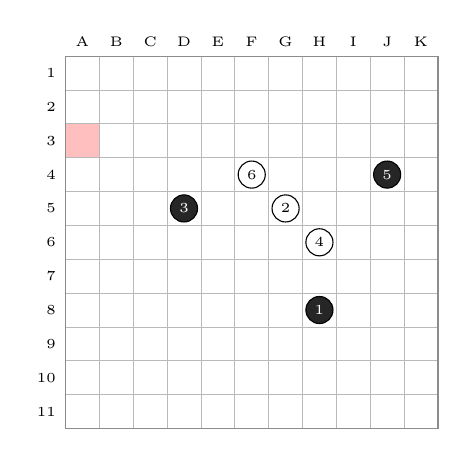
\begin{tikzpicture}[x=0.43cm, y=0.43cm]
\fill[red!25] (0,-2) rectangle (1,-3);
\draw[gray!55, line width=.3pt, step=1] (0,0) grid (11,-11);
\draw[gray!90] (0,0) rectangle (11,-11);
\node[font=\tiny, anchor=south] at (0.5,0) {A};
\node[font=\tiny, anchor=south] at (1.5,0) {B};
\node[font=\tiny, anchor=south] at (2.5,0) {C};
\node[font=\tiny, anchor=south] at (3.5,0) {D};
\node[font=\tiny, anchor=south] at (4.5,0) {E};
\node[font=\tiny, anchor=south] at (5.5,0) {F};
\node[font=\tiny, anchor=south] at (6.5,0) {G};
\node[font=\tiny, anchor=south] at (7.5,0) {H};
\node[font=\tiny, anchor=south] at (8.5,0) {I};
\node[font=\tiny, anchor=south] at (9.5,0) {J};
\node[font=\tiny, anchor=south] at (10.5,0) {K};
\node[font=\tiny, anchor=east] at (0,-0.5) {1};
\node[font=\tiny, anchor=east] at (0,-1.5) {2};
\node[font=\tiny, anchor=east] at (0,-2.5) {3};
\node[font=\tiny, anchor=east] at (0,-3.5) {4};
\node[font=\tiny, anchor=east] at (0,-4.5) {5};
\node[font=\tiny, anchor=east] at (0,-5.5) {6};
\node[font=\tiny, anchor=east] at (0,-6.5) {7};
\node[font=\tiny, anchor=east] at (0,-7.5) {8};
\node[font=\tiny, anchor=east] at (0,-8.5) {9};
\node[font=\tiny, anchor=east] at (0,-9.5) {10};
\node[font=\tiny, anchor=east] at (0,-10.5) {11};
\draw[fill=white, line width=.4pt] (5.5,-3.5) circle (.40);
\node[font=\tiny, text=black, inner sep=0pt] at (5.5,-3.5) {6};
\draw[fill=black!85, line width=.4pt] (9.5,-3.5) circle (.40);
\node[font=\tiny, text=white, inner sep=0pt] at (9.5,-3.5) {5};
\draw[fill=black!85, line width=.4pt] (3.5,-4.5) circle (.40);
\node[font=\tiny, text=white, inner sep=0pt] at (3.5,-4.5) {3};
\draw[fill=white, line width=.4pt] (6.5,-4.5) circle (.40);
\node[font=\tiny, text=black, inner sep=0pt] at (6.5,-4.5) {2};
\draw[fill=white, line width=.4pt] (7.5,-5.5) circle (.40);
\node[font=\tiny, text=black, inner sep=0pt] at (7.5,-5.5) {4};
\draw[fill=black!85, line width=.4pt] (7.5,-7.5) circle (.40);
\node[font=\tiny, text=white, inner sep=0pt] at (7.5,-7.5) {1};
\end{tikzpicture}
    \caption{Trước nước 7 (X đi; ô đỏ là nước đã chọn)}
  \end{subfigure}\hfill
  \begin{subfigure}[t]{.48\linewidth}
    \centering
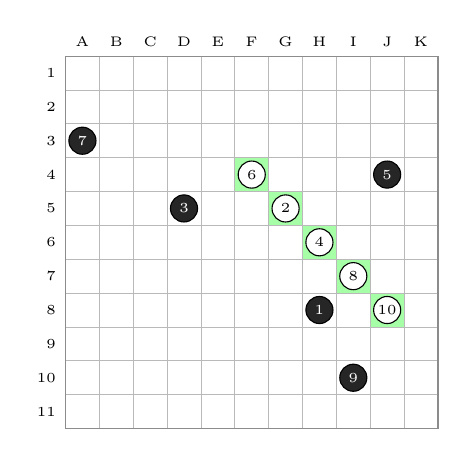
\begin{tikzpicture}[x=0.43cm, y=0.43cm]
\fill[green!35] (9,-7) rectangle (10,-8);
\fill[green!35] (8,-6) rectangle (9,-7);
\fill[green!35] (7,-5) rectangle (8,-6);
\fill[green!35] (6,-4) rectangle (7,-5);
\fill[green!35] (5,-3) rectangle (6,-4);
\draw[gray!55, line width=.3pt, step=1] (0,0) grid (11,-11);
\draw[gray!90] (0,0) rectangle (11,-11);
\node[font=\tiny, anchor=south] at (0.5,0) {A};
\node[font=\tiny, anchor=south] at (1.5,0) {B};
\node[font=\tiny, anchor=south] at (2.5,0) {C};
\node[font=\tiny, anchor=south] at (3.5,0) {D};
\node[font=\tiny, anchor=south] at (4.5,0) {E};
\node[font=\tiny, anchor=south] at (5.5,0) {F};
\node[font=\tiny, anchor=south] at (6.5,0) {G};
\node[font=\tiny, anchor=south] at (7.5,0) {H};
\node[font=\tiny, anchor=south] at (8.5,0) {I};
\node[font=\tiny, anchor=south] at (9.5,0) {J};
\node[font=\tiny, anchor=south] at (10.5,0) {K};
\node[font=\tiny, anchor=east] at (0,-0.5) {1};
\node[font=\tiny, anchor=east] at (0,-1.5) {2};
\node[font=\tiny, anchor=east] at (0,-2.5) {3};
\node[font=\tiny, anchor=east] at (0,-3.5) {4};
\node[font=\tiny, anchor=east] at (0,-4.5) {5};
\node[font=\tiny, anchor=east] at (0,-5.5) {6};
\node[font=\tiny, anchor=east] at (0,-6.5) {7};
\node[font=\tiny, anchor=east] at (0,-7.5) {8};
\node[font=\tiny, anchor=east] at (0,-8.5) {9};
\node[font=\tiny, anchor=east] at (0,-9.5) {10};
\node[font=\tiny, anchor=east] at (0,-10.5) {11};
\draw[fill=black!85, line width=.4pt] (0.5,-2.5) circle (.40);
\node[font=\tiny, text=white, inner sep=0pt] at (0.5,-2.5) {7};
\draw[fill=white, line width=.4pt] (5.5,-3.5) circle (.40);
\node[font=\tiny, text=black, inner sep=0pt] at (5.5,-3.5) {6};
\draw[fill=black!85, line width=.4pt] (9.5,-3.5) circle (.40);
\node[font=\tiny, text=white, inner sep=0pt] at (9.5,-3.5) {5};
\draw[fill=black!85, line width=.4pt] (3.5,-4.5) circle (.40);
\node[font=\tiny, text=white, inner sep=0pt] at (3.5,-4.5) {3};
\draw[fill=white, line width=.4pt] (6.5,-4.5) circle (.40);
\node[font=\tiny, text=black, inner sep=0pt] at (6.5,-4.5) {2};
\draw[fill=white, line width=.4pt] (7.5,-5.5) circle (.40);
\node[font=\tiny, text=black, inner sep=0pt] at (7.5,-5.5) {4};
\draw[fill=white, line width=.4pt] (8.5,-6.5) circle (.40);
\node[font=\tiny, text=black, inner sep=0pt] at (8.5,-6.5) {8};
\draw[fill=black!85, line width=.4pt] (7.5,-7.5) circle (.40);
\node[font=\tiny, text=white, inner sep=0pt] at (7.5,-7.5) {1};
\draw[fill=white, line width=.4pt] (9.5,-7.5) circle (.40);
\node[font=\tiny, text=black, inner sep=0pt] at (9.5,-7.5) {10};
\draw[fill=black!85, line width=.4pt] (8.5,-9.5) circle (.40);
\node[font=\tiny, text=white, inner sep=0pt] at (8.5,-9.5) {9};
\end{tikzpicture}
    \caption{Thế cuối (ô xanh: dãy thắng)}
  \end{subfigure}
  \caption{Ván 370 (L1 cầm X, L5 cầm O).}
  \label{fig:cs-van-04}
\end{figure}
{\footnotesize\linespread{1}\selectfont
\noindent\begin{tabularx}{\linewidth}{*{6}{X}}
\toprule
1.~X H8$^\ast$ & 3.~X D5 & 5.~X J4 & 7.~X A3 & 9.~X I10 &  \\
2.~O G5$^\ast$ & 4.~O H6 & 6.~O F4 & 8.~O I7 & 10.~O J8 &  \\
\bottomrule
\end{tabularx}\par}
\paragraph{Diễn biến chiến thuật.}
\begin{itemize}\small
\setlength{\itemsep}{0pt}
  \item Nước 7 (X=L1, A3): để đối thủ có VCF: E3--D2--I7.
  \item Nước 8 (O=L5, I7): đang có VCF 2 nước và đi đúng một đường (E3--D2--I7 là đường ngắn nhất).
  \item Nước 9 (X=L1, I10): đối thủ đang có các ô thắng E3, J8, không đỡ hết được.
  \item Nước 10 (O=L5, J8): thắng ngay.
\end{itemize}
Thời gian trung vị mỗi nước: X 0,0 ms, O 1,3 ms.
\clearpage

\subsection{L1 -- L6: ván 495}
\label{sec:cs-van-05}
X: \texttt{L6-PolicyRL}; O: \texttt{L1-Random}; khai cuộc 47 (4 nước, đánh dấu $\ast$); 11 nước; kết quả: X (L6) thắng. Cả cặp: L1 thắng 0, hoà 0, thua 100 trên 100 ván; trung vị 11 nước.
\begin{figure}[H]
  \centering
  \begin{subfigure}[t]{.48\linewidth}
    \centering
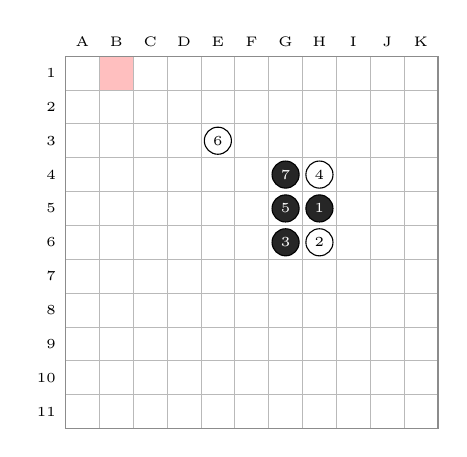
\begin{tikzpicture}[x=0.43cm, y=0.43cm]
\fill[red!25] (1,0) rectangle (2,-1);
\draw[gray!55, line width=.3pt, step=1] (0,0) grid (11,-11);
\draw[gray!90] (0,0) rectangle (11,-11);
\node[font=\tiny, anchor=south] at (0.5,0) {A};
\node[font=\tiny, anchor=south] at (1.5,0) {B};
\node[font=\tiny, anchor=south] at (2.5,0) {C};
\node[font=\tiny, anchor=south] at (3.5,0) {D};
\node[font=\tiny, anchor=south] at (4.5,0) {E};
\node[font=\tiny, anchor=south] at (5.5,0) {F};
\node[font=\tiny, anchor=south] at (6.5,0) {G};
\node[font=\tiny, anchor=south] at (7.5,0) {H};
\node[font=\tiny, anchor=south] at (8.5,0) {I};
\node[font=\tiny, anchor=south] at (9.5,0) {J};
\node[font=\tiny, anchor=south] at (10.5,0) {K};
\node[font=\tiny, anchor=east] at (0,-0.5) {1};
\node[font=\tiny, anchor=east] at (0,-1.5) {2};
\node[font=\tiny, anchor=east] at (0,-2.5) {3};
\node[font=\tiny, anchor=east] at (0,-3.5) {4};
\node[font=\tiny, anchor=east] at (0,-4.5) {5};
\node[font=\tiny, anchor=east] at (0,-5.5) {6};
\node[font=\tiny, anchor=east] at (0,-6.5) {7};
\node[font=\tiny, anchor=east] at (0,-7.5) {8};
\node[font=\tiny, anchor=east] at (0,-8.5) {9};
\node[font=\tiny, anchor=east] at (0,-9.5) {10};
\node[font=\tiny, anchor=east] at (0,-10.5) {11};
\draw[fill=white, line width=.4pt] (4.5,-2.5) circle (.40);
\node[font=\tiny, text=black, inner sep=0pt] at (4.5,-2.5) {6};
\draw[fill=black!85, line width=.4pt] (6.5,-3.5) circle (.40);
\node[font=\tiny, text=white, inner sep=0pt] at (6.5,-3.5) {7};
\draw[fill=white, line width=.4pt] (7.5,-3.5) circle (.40);
\node[font=\tiny, text=black, inner sep=0pt] at (7.5,-3.5) {4};
\draw[fill=black!85, line width=.4pt] (6.5,-4.5) circle (.40);
\node[font=\tiny, text=white, inner sep=0pt] at (6.5,-4.5) {5};
\draw[fill=black!85, line width=.4pt] (7.5,-4.5) circle (.40);
\node[font=\tiny, text=white, inner sep=0pt] at (7.5,-4.5) {1};
\draw[fill=black!85, line width=.4pt] (6.5,-5.5) circle (.40);
\node[font=\tiny, text=white, inner sep=0pt] at (6.5,-5.5) {3};
\draw[fill=white, line width=.4pt] (7.5,-5.5) circle (.40);
\node[font=\tiny, text=black, inner sep=0pt] at (7.5,-5.5) {2};
\end{tikzpicture}
    \caption{Trước nước 8 (O đi; ô đỏ là nước đã chọn)}
  \end{subfigure}\hfill
  \begin{subfigure}[t]{.48\linewidth}
    \centering
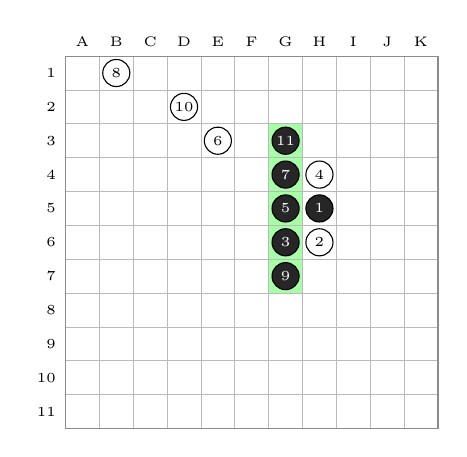
\begin{tikzpicture}[x=0.43cm, y=0.43cm]
\fill[green!35] (6,-2) rectangle (7,-3);
\fill[green!35] (6,-3) rectangle (7,-4);
\fill[green!35] (6,-4) rectangle (7,-5);
\fill[green!35] (6,-5) rectangle (7,-6);
\fill[green!35] (6,-6) rectangle (7,-7);
\draw[gray!55, line width=.3pt, step=1] (0,0) grid (11,-11);
\draw[gray!90] (0,0) rectangle (11,-11);
\node[font=\tiny, anchor=south] at (0.5,0) {A};
\node[font=\tiny, anchor=south] at (1.5,0) {B};
\node[font=\tiny, anchor=south] at (2.5,0) {C};
\node[font=\tiny, anchor=south] at (3.5,0) {D};
\node[font=\tiny, anchor=south] at (4.5,0) {E};
\node[font=\tiny, anchor=south] at (5.5,0) {F};
\node[font=\tiny, anchor=south] at (6.5,0) {G};
\node[font=\tiny, anchor=south] at (7.5,0) {H};
\node[font=\tiny, anchor=south] at (8.5,0) {I};
\node[font=\tiny, anchor=south] at (9.5,0) {J};
\node[font=\tiny, anchor=south] at (10.5,0) {K};
\node[font=\tiny, anchor=east] at (0,-0.5) {1};
\node[font=\tiny, anchor=east] at (0,-1.5) {2};
\node[font=\tiny, anchor=east] at (0,-2.5) {3};
\node[font=\tiny, anchor=east] at (0,-3.5) {4};
\node[font=\tiny, anchor=east] at (0,-4.5) {5};
\node[font=\tiny, anchor=east] at (0,-5.5) {6};
\node[font=\tiny, anchor=east] at (0,-6.5) {7};
\node[font=\tiny, anchor=east] at (0,-7.5) {8};
\node[font=\tiny, anchor=east] at (0,-8.5) {9};
\node[font=\tiny, anchor=east] at (0,-9.5) {10};
\node[font=\tiny, anchor=east] at (0,-10.5) {11};
\draw[fill=white, line width=.4pt] (1.5,-0.5) circle (.40);
\node[font=\tiny, text=black, inner sep=0pt] at (1.5,-0.5) {8};
\draw[fill=white, line width=.4pt] (3.5,-1.5) circle (.40);
\node[font=\tiny, text=black, inner sep=0pt] at (3.5,-1.5) {10};
\draw[fill=white, line width=.4pt] (4.5,-2.5) circle (.40);
\node[font=\tiny, text=black, inner sep=0pt] at (4.5,-2.5) {6};
\draw[fill=black!85, line width=.4pt] (6.5,-2.5) circle (.40);
\node[font=\tiny, text=white, inner sep=0pt] at (6.5,-2.5) {11};
\draw[fill=black!85, line width=.4pt] (6.5,-3.5) circle (.40);
\node[font=\tiny, text=white, inner sep=0pt] at (6.5,-3.5) {7};
\draw[fill=white, line width=.4pt] (7.5,-3.5) circle (.40);
\node[font=\tiny, text=black, inner sep=0pt] at (7.5,-3.5) {4};
\draw[fill=black!85, line width=.4pt] (6.5,-4.5) circle (.40);
\node[font=\tiny, text=white, inner sep=0pt] at (6.5,-4.5) {5};
\draw[fill=black!85, line width=.4pt] (7.5,-4.5) circle (.40);
\node[font=\tiny, text=white, inner sep=0pt] at (7.5,-4.5) {1};
\draw[fill=black!85, line width=.4pt] (6.5,-5.5) circle (.40);
\node[font=\tiny, text=white, inner sep=0pt] at (6.5,-5.5) {3};
\draw[fill=white, line width=.4pt] (7.5,-5.5) circle (.40);
\node[font=\tiny, text=black, inner sep=0pt] at (7.5,-5.5) {2};
\draw[fill=black!85, line width=.4pt] (6.5,-6.5) circle (.40);
\node[font=\tiny, text=white, inner sep=0pt] at (6.5,-6.5) {9};
\end{tikzpicture}
    \caption{Thế cuối (ô xanh: dãy thắng)}
  \end{subfigure}
  \caption{Ván 495 (L6 cầm X, L1 cầm O).}
  \label{fig:cs-van-05}
\end{figure}
{\footnotesize\linespread{1}\selectfont
\noindent\begin{tabularx}{\linewidth}{*{6}{X}}
\toprule
1.~X H5$^\ast$ & 3.~X G6$^\ast$ & 5.~X G5 & 7.~X G4 & 9.~X G7 & 11.~X G3 \\
2.~O H6$^\ast$ & 4.~O H4$^\ast$ & 6.~O E3 & 8.~O B1 & 10.~O D2 &  \\
\bottomrule
\end{tabularx}\par}
\paragraph{Diễn biến chiến thuật.}
\begin{itemize}\small
\setlength{\itemsep}{0pt}
  \item Nước 8 (O=L1, B1): để đối thủ có VCF: G3--G2--G7.
  \item Nước 9 (X=L6, G7): đang có VCF 2 nước và đi đúng một đường (G3--G2--G7 là đường ngắn nhất).
  \item Nước 10 (O=L1, D2): đối thủ đang có các ô thắng G3, G8, không đỡ hết được.
  \item Nước 11 (X=L6, G3): thắng ngay.
\end{itemize}
Thời gian trung vị mỗi nước: X 1,2 ms, O 0,0 ms.
\clearpage

\subsection{L1 -- L7: ván 570}
\label{sec:cs-van-06}
X: \texttt{L1-Random}; O: \texttt{L7-PUCT}; khai cuộc 35 (2 nước, đánh dấu $\ast$); 10 nước; kết quả: O (L7) thắng. Cả cặp: L1 thắng 0, hoà 0, thua 100 trên 100 ván; trung vị 10 nước.
\begin{figure}[H]
  \centering
  \begin{subfigure}[t]{.48\linewidth}
    \centering
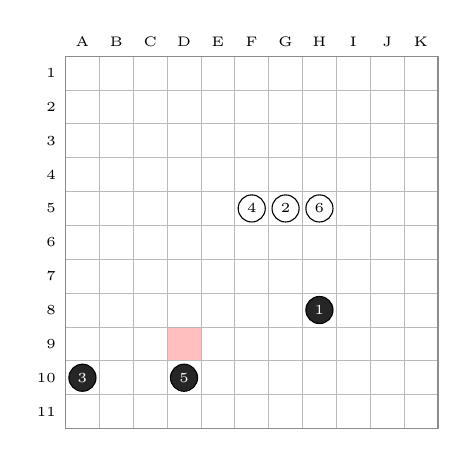
\begin{tikzpicture}[x=0.43cm, y=0.43cm]
\fill[red!25] (3,-8) rectangle (4,-9);
\draw[gray!55, line width=.3pt, step=1] (0,0) grid (11,-11);
\draw[gray!90] (0,0) rectangle (11,-11);
\node[font=\tiny, anchor=south] at (0.5,0) {A};
\node[font=\tiny, anchor=south] at (1.5,0) {B};
\node[font=\tiny, anchor=south] at (2.5,0) {C};
\node[font=\tiny, anchor=south] at (3.5,0) {D};
\node[font=\tiny, anchor=south] at (4.5,0) {E};
\node[font=\tiny, anchor=south] at (5.5,0) {F};
\node[font=\tiny, anchor=south] at (6.5,0) {G};
\node[font=\tiny, anchor=south] at (7.5,0) {H};
\node[font=\tiny, anchor=south] at (8.5,0) {I};
\node[font=\tiny, anchor=south] at (9.5,0) {J};
\node[font=\tiny, anchor=south] at (10.5,0) {K};
\node[font=\tiny, anchor=east] at (0,-0.5) {1};
\node[font=\tiny, anchor=east] at (0,-1.5) {2};
\node[font=\tiny, anchor=east] at (0,-2.5) {3};
\node[font=\tiny, anchor=east] at (0,-3.5) {4};
\node[font=\tiny, anchor=east] at (0,-4.5) {5};
\node[font=\tiny, anchor=east] at (0,-5.5) {6};
\node[font=\tiny, anchor=east] at (0,-6.5) {7};
\node[font=\tiny, anchor=east] at (0,-7.5) {8};
\node[font=\tiny, anchor=east] at (0,-8.5) {9};
\node[font=\tiny, anchor=east] at (0,-9.5) {10};
\node[font=\tiny, anchor=east] at (0,-10.5) {11};
\draw[fill=white, line width=.4pt] (5.5,-4.5) circle (.40);
\node[font=\tiny, text=black, inner sep=0pt] at (5.5,-4.5) {4};
\draw[fill=white, line width=.4pt] (6.5,-4.5) circle (.40);
\node[font=\tiny, text=black, inner sep=0pt] at (6.5,-4.5) {2};
\draw[fill=white, line width=.4pt] (7.5,-4.5) circle (.40);
\node[font=\tiny, text=black, inner sep=0pt] at (7.5,-4.5) {6};
\draw[fill=black!85, line width=.4pt] (7.5,-7.5) circle (.40);
\node[font=\tiny, text=white, inner sep=0pt] at (7.5,-7.5) {1};
\draw[fill=black!85, line width=.4pt] (0.5,-9.5) circle (.40);
\node[font=\tiny, text=white, inner sep=0pt] at (0.5,-9.5) {3};
\draw[fill=black!85, line width=.4pt] (3.5,-9.5) circle (.40);
\node[font=\tiny, text=white, inner sep=0pt] at (3.5,-9.5) {5};
\end{tikzpicture}
    \caption{Trước nước 7 (X đi; ô đỏ là nước đã chọn)}
  \end{subfigure}\hfill
  \begin{subfigure}[t]{.48\linewidth}
    \centering
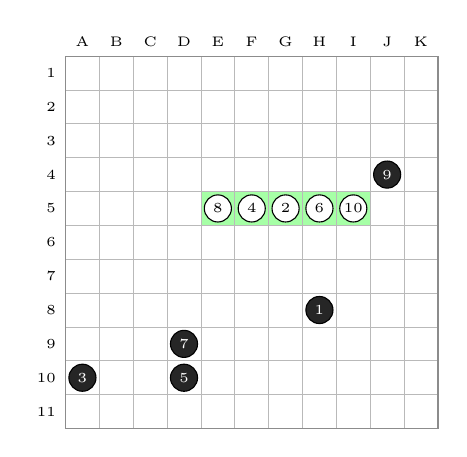
\begin{tikzpicture}[x=0.43cm, y=0.43cm]
\fill[green!35] (8,-4) rectangle (9,-5);
\fill[green!35] (7,-4) rectangle (8,-5);
\fill[green!35] (6,-4) rectangle (7,-5);
\fill[green!35] (5,-4) rectangle (6,-5);
\fill[green!35] (4,-4) rectangle (5,-5);
\draw[gray!55, line width=.3pt, step=1] (0,0) grid (11,-11);
\draw[gray!90] (0,0) rectangle (11,-11);
\node[font=\tiny, anchor=south] at (0.5,0) {A};
\node[font=\tiny, anchor=south] at (1.5,0) {B};
\node[font=\tiny, anchor=south] at (2.5,0) {C};
\node[font=\tiny, anchor=south] at (3.5,0) {D};
\node[font=\tiny, anchor=south] at (4.5,0) {E};
\node[font=\tiny, anchor=south] at (5.5,0) {F};
\node[font=\tiny, anchor=south] at (6.5,0) {G};
\node[font=\tiny, anchor=south] at (7.5,0) {H};
\node[font=\tiny, anchor=south] at (8.5,0) {I};
\node[font=\tiny, anchor=south] at (9.5,0) {J};
\node[font=\tiny, anchor=south] at (10.5,0) {K};
\node[font=\tiny, anchor=east] at (0,-0.5) {1};
\node[font=\tiny, anchor=east] at (0,-1.5) {2};
\node[font=\tiny, anchor=east] at (0,-2.5) {3};
\node[font=\tiny, anchor=east] at (0,-3.5) {4};
\node[font=\tiny, anchor=east] at (0,-4.5) {5};
\node[font=\tiny, anchor=east] at (0,-5.5) {6};
\node[font=\tiny, anchor=east] at (0,-6.5) {7};
\node[font=\tiny, anchor=east] at (0,-7.5) {8};
\node[font=\tiny, anchor=east] at (0,-8.5) {9};
\node[font=\tiny, anchor=east] at (0,-9.5) {10};
\node[font=\tiny, anchor=east] at (0,-10.5) {11};
\draw[fill=black!85, line width=.4pt] (9.5,-3.5) circle (.40);
\node[font=\tiny, text=white, inner sep=0pt] at (9.5,-3.5) {9};
\draw[fill=white, line width=.4pt] (4.5,-4.5) circle (.40);
\node[font=\tiny, text=black, inner sep=0pt] at (4.5,-4.5) {8};
\draw[fill=white, line width=.4pt] (5.5,-4.5) circle (.40);
\node[font=\tiny, text=black, inner sep=0pt] at (5.5,-4.5) {4};
\draw[fill=white, line width=.4pt] (6.5,-4.5) circle (.40);
\node[font=\tiny, text=black, inner sep=0pt] at (6.5,-4.5) {2};
\draw[fill=white, line width=.4pt] (7.5,-4.5) circle (.40);
\node[font=\tiny, text=black, inner sep=0pt] at (7.5,-4.5) {6};
\draw[fill=white, line width=.4pt] (8.5,-4.5) circle (.40);
\node[font=\tiny, text=black, inner sep=0pt] at (8.5,-4.5) {10};
\draw[fill=black!85, line width=.4pt] (7.5,-7.5) circle (.40);
\node[font=\tiny, text=white, inner sep=0pt] at (7.5,-7.5) {1};
\draw[fill=black!85, line width=.4pt] (3.5,-8.5) circle (.40);
\node[font=\tiny, text=white, inner sep=0pt] at (3.5,-8.5) {7};
\draw[fill=black!85, line width=.4pt] (0.5,-9.5) circle (.40);
\node[font=\tiny, text=white, inner sep=0pt] at (0.5,-9.5) {3};
\draw[fill=black!85, line width=.4pt] (3.5,-9.5) circle (.40);
\node[font=\tiny, text=white, inner sep=0pt] at (3.5,-9.5) {5};
\end{tikzpicture}
    \caption{Thế cuối (ô xanh: dãy thắng)}
  \end{subfigure}
  \caption{Ván 570 (L1 cầm X, L7 cầm O).}
  \label{fig:cs-van-06}
\end{figure}
{\footnotesize\linespread{1}\selectfont
\noindent\begin{tabularx}{\linewidth}{*{6}{X}}
\toprule
1.~X H8$^\ast$ & 3.~X A10 & 5.~X D10 & 7.~X D9 & 9.~X J4 &  \\
2.~O G5$^\ast$ & 4.~O F5 & 6.~O H5 & 8.~O E5 & 10.~O I5 &  \\
\bottomrule
\end{tabularx}\par}
\paragraph{Diễn biến chiến thuật.}
\begin{itemize}\small
\setlength{\itemsep}{0pt}
  \item Nước 7 (X=L1, D9): để đối thủ có VCF: E5--D5--I5.
  \item Nước 8 (O=L7, E5): đang có VCF 2 nước và đi đúng một đường (E5--D5--I5 là đường ngắn nhất).
  \item Nước 9 (X=L1, J4): đối thủ đang có các ô thắng D5, I5, không đỡ hết được.
  \item Nước 10 (O=L7, I5): thắng ngay.
\end{itemize}
Thời gian trung vị mỗi nước: X 0,0 ms, O 76,7 ms.
\clearpage

\subsection{L1 -- L8: ván 676}
\label{sec:cs-van-07}
X: \texttt{L1-Random}; O: \texttt{L8-AlphaZero}; khai cuộc 38 (3 nước, đánh dấu $\ast$); 10 nước; kết quả: O (L8) thắng. Cả cặp: L1 thắng 0, hoà 0, thua 100 trên 100 ván; trung vị 10 nước.
\begin{figure}[H]
  \centering
  \begin{subfigure}[t]{.48\linewidth}
    \centering
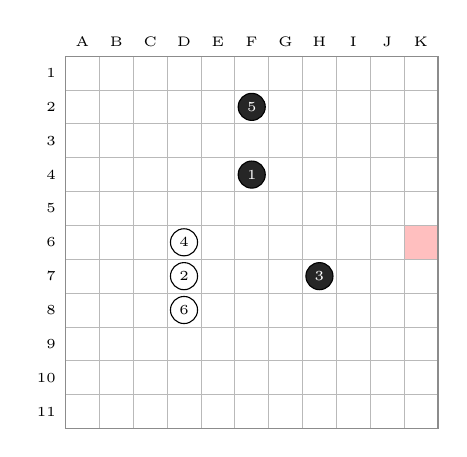
\begin{tikzpicture}[x=0.43cm, y=0.43cm]
\fill[red!25] (10,-5) rectangle (11,-6);
\draw[gray!55, line width=.3pt, step=1] (0,0) grid (11,-11);
\draw[gray!90] (0,0) rectangle (11,-11);
\node[font=\tiny, anchor=south] at (0.5,0) {A};
\node[font=\tiny, anchor=south] at (1.5,0) {B};
\node[font=\tiny, anchor=south] at (2.5,0) {C};
\node[font=\tiny, anchor=south] at (3.5,0) {D};
\node[font=\tiny, anchor=south] at (4.5,0) {E};
\node[font=\tiny, anchor=south] at (5.5,0) {F};
\node[font=\tiny, anchor=south] at (6.5,0) {G};
\node[font=\tiny, anchor=south] at (7.5,0) {H};
\node[font=\tiny, anchor=south] at (8.5,0) {I};
\node[font=\tiny, anchor=south] at (9.5,0) {J};
\node[font=\tiny, anchor=south] at (10.5,0) {K};
\node[font=\tiny, anchor=east] at (0,-0.5) {1};
\node[font=\tiny, anchor=east] at (0,-1.5) {2};
\node[font=\tiny, anchor=east] at (0,-2.5) {3};
\node[font=\tiny, anchor=east] at (0,-3.5) {4};
\node[font=\tiny, anchor=east] at (0,-4.5) {5};
\node[font=\tiny, anchor=east] at (0,-5.5) {6};
\node[font=\tiny, anchor=east] at (0,-6.5) {7};
\node[font=\tiny, anchor=east] at (0,-7.5) {8};
\node[font=\tiny, anchor=east] at (0,-8.5) {9};
\node[font=\tiny, anchor=east] at (0,-9.5) {10};
\node[font=\tiny, anchor=east] at (0,-10.5) {11};
\draw[fill=black!85, line width=.4pt] (5.5,-1.5) circle (.40);
\node[font=\tiny, text=white, inner sep=0pt] at (5.5,-1.5) {5};
\draw[fill=black!85, line width=.4pt] (5.5,-3.5) circle (.40);
\node[font=\tiny, text=white, inner sep=0pt] at (5.5,-3.5) {1};
\draw[fill=white, line width=.4pt] (3.5,-5.5) circle (.40);
\node[font=\tiny, text=black, inner sep=0pt] at (3.5,-5.5) {4};
\draw[fill=white, line width=.4pt] (3.5,-6.5) circle (.40);
\node[font=\tiny, text=black, inner sep=0pt] at (3.5,-6.5) {2};
\draw[fill=black!85, line width=.4pt] (7.5,-6.5) circle (.40);
\node[font=\tiny, text=white, inner sep=0pt] at (7.5,-6.5) {3};
\draw[fill=white, line width=.4pt] (3.5,-7.5) circle (.40);
\node[font=\tiny, text=black, inner sep=0pt] at (3.5,-7.5) {6};
\end{tikzpicture}
    \caption{Trước nước 7 (X đi; ô đỏ là nước đã chọn)}
  \end{subfigure}\hfill
  \begin{subfigure}[t]{.48\linewidth}
    \centering
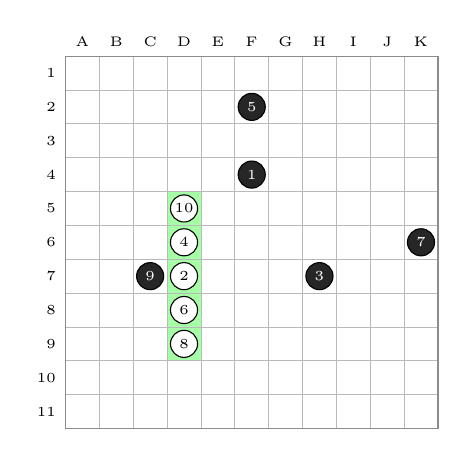
\begin{tikzpicture}[x=0.43cm, y=0.43cm]
\fill[green!35] (3,-4) rectangle (4,-5);
\fill[green!35] (3,-5) rectangle (4,-6);
\fill[green!35] (3,-6) rectangle (4,-7);
\fill[green!35] (3,-7) rectangle (4,-8);
\fill[green!35] (3,-8) rectangle (4,-9);
\draw[gray!55, line width=.3pt, step=1] (0,0) grid (11,-11);
\draw[gray!90] (0,0) rectangle (11,-11);
\node[font=\tiny, anchor=south] at (0.5,0) {A};
\node[font=\tiny, anchor=south] at (1.5,0) {B};
\node[font=\tiny, anchor=south] at (2.5,0) {C};
\node[font=\tiny, anchor=south] at (3.5,0) {D};
\node[font=\tiny, anchor=south] at (4.5,0) {E};
\node[font=\tiny, anchor=south] at (5.5,0) {F};
\node[font=\tiny, anchor=south] at (6.5,0) {G};
\node[font=\tiny, anchor=south] at (7.5,0) {H};
\node[font=\tiny, anchor=south] at (8.5,0) {I};
\node[font=\tiny, anchor=south] at (9.5,0) {J};
\node[font=\tiny, anchor=south] at (10.5,0) {K};
\node[font=\tiny, anchor=east] at (0,-0.5) {1};
\node[font=\tiny, anchor=east] at (0,-1.5) {2};
\node[font=\tiny, anchor=east] at (0,-2.5) {3};
\node[font=\tiny, anchor=east] at (0,-3.5) {4};
\node[font=\tiny, anchor=east] at (0,-4.5) {5};
\node[font=\tiny, anchor=east] at (0,-5.5) {6};
\node[font=\tiny, anchor=east] at (0,-6.5) {7};
\node[font=\tiny, anchor=east] at (0,-7.5) {8};
\node[font=\tiny, anchor=east] at (0,-8.5) {9};
\node[font=\tiny, anchor=east] at (0,-9.5) {10};
\node[font=\tiny, anchor=east] at (0,-10.5) {11};
\draw[fill=black!85, line width=.4pt] (5.5,-1.5) circle (.40);
\node[font=\tiny, text=white, inner sep=0pt] at (5.5,-1.5) {5};
\draw[fill=black!85, line width=.4pt] (5.5,-3.5) circle (.40);
\node[font=\tiny, text=white, inner sep=0pt] at (5.5,-3.5) {1};
\draw[fill=white, line width=.4pt] (3.5,-4.5) circle (.40);
\node[font=\tiny, text=black, inner sep=0pt] at (3.5,-4.5) {10};
\draw[fill=white, line width=.4pt] (3.5,-5.5) circle (.40);
\node[font=\tiny, text=black, inner sep=0pt] at (3.5,-5.5) {4};
\draw[fill=black!85, line width=.4pt] (10.5,-5.5) circle (.40);
\node[font=\tiny, text=white, inner sep=0pt] at (10.5,-5.5) {7};
\draw[fill=black!85, line width=.4pt] (2.5,-6.5) circle (.40);
\node[font=\tiny, text=white, inner sep=0pt] at (2.5,-6.5) {9};
\draw[fill=white, line width=.4pt] (3.5,-6.5) circle (.40);
\node[font=\tiny, text=black, inner sep=0pt] at (3.5,-6.5) {2};
\draw[fill=black!85, line width=.4pt] (7.5,-6.5) circle (.40);
\node[font=\tiny, text=white, inner sep=0pt] at (7.5,-6.5) {3};
\draw[fill=white, line width=.4pt] (3.5,-7.5) circle (.40);
\node[font=\tiny, text=black, inner sep=0pt] at (3.5,-7.5) {6};
\draw[fill=white, line width=.4pt] (3.5,-8.5) circle (.40);
\node[font=\tiny, text=black, inner sep=0pt] at (3.5,-8.5) {8};
\end{tikzpicture}
    \caption{Thế cuối (ô xanh: dãy thắng)}
  \end{subfigure}
  \caption{Ván 676 (L1 cầm X, L8 cầm O).}
  \label{fig:cs-van-07}
\end{figure}
{\footnotesize\linespread{1}\selectfont
\noindent\begin{tabularx}{\linewidth}{*{6}{X}}
\toprule
1.~X F4$^\ast$ & 3.~X H7$^\ast$ & 5.~X F2 & 7.~X K6 & 9.~X C7 &  \\
2.~O D7$^\ast$ & 4.~O D6 & 6.~O D8 & 8.~O D9 & 10.~O D5 &  \\
\bottomrule
\end{tabularx}\par}
\paragraph{Diễn biến chiến thuật.}
\begin{itemize}\small
\setlength{\itemsep}{0pt}
  \item Nước 7 (X=L1, K6): để đối thủ có VCF: D5--D4--D9.
  \item Nước 8 (O=L8, D9): đang có VCF 2 nước và đi đúng một đường (D5--D4--D9 là đường ngắn nhất).
  \item Nước 9 (X=L1, C7): đối thủ đang có các ô thắng D5, D10, không đỡ hết được.
  \item Nước 10 (O=L8, D5): thắng ngay.
\end{itemize}
Thời gian trung vị mỗi nước: X 0,0 ms, O 95,3 ms.
\clearpage

\subsection{L2 -- L3: ván 790}
\label{sec:cs-van-08}
X: \texttt{L2-Rule}; O: \texttt{L3-AlphaBeta}; khai cuộc 45 (3 nước, đánh dấu $\ast$); 28 nước; kết quả: O (L3) thắng. Cả cặp: L2 thắng 31, hoà 3, thua 66 trên 100 ván; trung vị 29 nước.
\begin{figure}[H]
  \centering
  \begin{subfigure}[t]{.48\linewidth}
    \centering
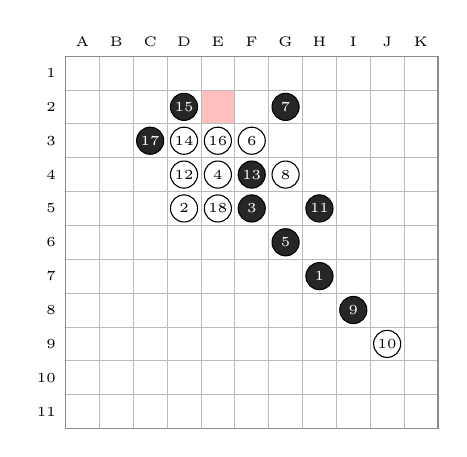
\begin{tikzpicture}[x=0.43cm, y=0.43cm]
\fill[red!25] (4,-1) rectangle (5,-2);
\draw[gray!55, line width=.3pt, step=1] (0,0) grid (11,-11);
\draw[gray!90] (0,0) rectangle (11,-11);
\node[font=\tiny, anchor=south] at (0.5,0) {A};
\node[font=\tiny, anchor=south] at (1.5,0) {B};
\node[font=\tiny, anchor=south] at (2.5,0) {C};
\node[font=\tiny, anchor=south] at (3.5,0) {D};
\node[font=\tiny, anchor=south] at (4.5,0) {E};
\node[font=\tiny, anchor=south] at (5.5,0) {F};
\node[font=\tiny, anchor=south] at (6.5,0) {G};
\node[font=\tiny, anchor=south] at (7.5,0) {H};
\node[font=\tiny, anchor=south] at (8.5,0) {I};
\node[font=\tiny, anchor=south] at (9.5,0) {J};
\node[font=\tiny, anchor=south] at (10.5,0) {K};
\node[font=\tiny, anchor=east] at (0,-0.5) {1};
\node[font=\tiny, anchor=east] at (0,-1.5) {2};
\node[font=\tiny, anchor=east] at (0,-2.5) {3};
\node[font=\tiny, anchor=east] at (0,-3.5) {4};
\node[font=\tiny, anchor=east] at (0,-4.5) {5};
\node[font=\tiny, anchor=east] at (0,-5.5) {6};
\node[font=\tiny, anchor=east] at (0,-6.5) {7};
\node[font=\tiny, anchor=east] at (0,-7.5) {8};
\node[font=\tiny, anchor=east] at (0,-8.5) {9};
\node[font=\tiny, anchor=east] at (0,-9.5) {10};
\node[font=\tiny, anchor=east] at (0,-10.5) {11};
\draw[fill=black!85, line width=.4pt] (3.5,-1.5) circle (.40);
\node[font=\tiny, text=white, inner sep=0pt] at (3.5,-1.5) {15};
\draw[fill=black!85, line width=.4pt] (6.5,-1.5) circle (.40);
\node[font=\tiny, text=white, inner sep=0pt] at (6.5,-1.5) {7};
\draw[fill=black!85, line width=.4pt] (2.5,-2.5) circle (.40);
\node[font=\tiny, text=white, inner sep=0pt] at (2.5,-2.5) {17};
\draw[fill=white, line width=.4pt] (3.5,-2.5) circle (.40);
\node[font=\tiny, text=black, inner sep=0pt] at (3.5,-2.5) {14};
\draw[fill=white, line width=.4pt] (4.5,-2.5) circle (.40);
\node[font=\tiny, text=black, inner sep=0pt] at (4.5,-2.5) {16};
\draw[fill=white, line width=.4pt] (5.5,-2.5) circle (.40);
\node[font=\tiny, text=black, inner sep=0pt] at (5.5,-2.5) {6};
\draw[fill=white, line width=.4pt] (3.5,-3.5) circle (.40);
\node[font=\tiny, text=black, inner sep=0pt] at (3.5,-3.5) {12};
\draw[fill=white, line width=.4pt] (4.5,-3.5) circle (.40);
\node[font=\tiny, text=black, inner sep=0pt] at (4.5,-3.5) {4};
\draw[fill=black!85, line width=.4pt] (5.5,-3.5) circle (.40);
\node[font=\tiny, text=white, inner sep=0pt] at (5.5,-3.5) {13};
\draw[fill=white, line width=.4pt] (6.5,-3.5) circle (.40);
\node[font=\tiny, text=black, inner sep=0pt] at (6.5,-3.5) {8};
\draw[fill=white, line width=.4pt] (3.5,-4.5) circle (.40);
\node[font=\tiny, text=black, inner sep=0pt] at (3.5,-4.5) {2};
\draw[fill=white, line width=.4pt] (4.5,-4.5) circle (.40);
\node[font=\tiny, text=black, inner sep=0pt] at (4.5,-4.5) {18};
\draw[fill=black!85, line width=.4pt] (5.5,-4.5) circle (.40);
\node[font=\tiny, text=white, inner sep=0pt] at (5.5,-4.5) {3};
\draw[fill=black!85, line width=.4pt] (7.5,-4.5) circle (.40);
\node[font=\tiny, text=white, inner sep=0pt] at (7.5,-4.5) {11};
\draw[fill=black!85, line width=.4pt] (6.5,-5.5) circle (.40);
\node[font=\tiny, text=white, inner sep=0pt] at (6.5,-5.5) {5};
\draw[fill=black!85, line width=.4pt] (7.5,-6.5) circle (.40);
\node[font=\tiny, text=white, inner sep=0pt] at (7.5,-6.5) {1};
\draw[fill=black!85, line width=.4pt] (8.5,-7.5) circle (.40);
\node[font=\tiny, text=white, inner sep=0pt] at (8.5,-7.5) {9};
\draw[fill=white, line width=.4pt] (9.5,-8.5) circle (.40);
\node[font=\tiny, text=black, inner sep=0pt] at (9.5,-8.5) {10};
\end{tikzpicture}
    \caption{Trước nước 19 (X đi; ô đỏ là nước đã chọn)}
  \end{subfigure}\hfill
  \begin{subfigure}[t]{.48\linewidth}
    \centering
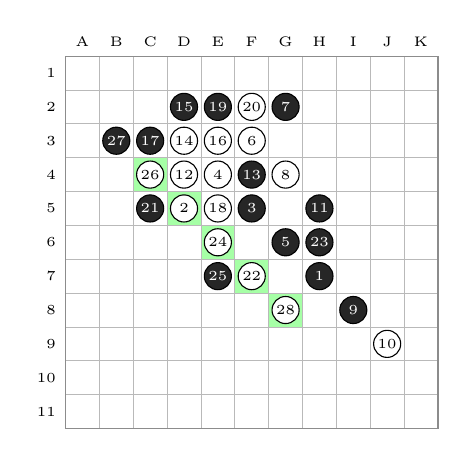
\begin{tikzpicture}[x=0.43cm, y=0.43cm]
\fill[green!35] (6,-7) rectangle (7,-8);
\fill[green!35] (5,-6) rectangle (6,-7);
\fill[green!35] (4,-5) rectangle (5,-6);
\fill[green!35] (3,-4) rectangle (4,-5);
\fill[green!35] (2,-3) rectangle (3,-4);
\draw[gray!55, line width=.3pt, step=1] (0,0) grid (11,-11);
\draw[gray!90] (0,0) rectangle (11,-11);
\node[font=\tiny, anchor=south] at (0.5,0) {A};
\node[font=\tiny, anchor=south] at (1.5,0) {B};
\node[font=\tiny, anchor=south] at (2.5,0) {C};
\node[font=\tiny, anchor=south] at (3.5,0) {D};
\node[font=\tiny, anchor=south] at (4.5,0) {E};
\node[font=\tiny, anchor=south] at (5.5,0) {F};
\node[font=\tiny, anchor=south] at (6.5,0) {G};
\node[font=\tiny, anchor=south] at (7.5,0) {H};
\node[font=\tiny, anchor=south] at (8.5,0) {I};
\node[font=\tiny, anchor=south] at (9.5,0) {J};
\node[font=\tiny, anchor=south] at (10.5,0) {K};
\node[font=\tiny, anchor=east] at (0,-0.5) {1};
\node[font=\tiny, anchor=east] at (0,-1.5) {2};
\node[font=\tiny, anchor=east] at (0,-2.5) {3};
\node[font=\tiny, anchor=east] at (0,-3.5) {4};
\node[font=\tiny, anchor=east] at (0,-4.5) {5};
\node[font=\tiny, anchor=east] at (0,-5.5) {6};
\node[font=\tiny, anchor=east] at (0,-6.5) {7};
\node[font=\tiny, anchor=east] at (0,-7.5) {8};
\node[font=\tiny, anchor=east] at (0,-8.5) {9};
\node[font=\tiny, anchor=east] at (0,-9.5) {10};
\node[font=\tiny, anchor=east] at (0,-10.5) {11};
\draw[fill=black!85, line width=.4pt] (3.5,-1.5) circle (.40);
\node[font=\tiny, text=white, inner sep=0pt] at (3.5,-1.5) {15};
\draw[fill=black!85, line width=.4pt] (4.5,-1.5) circle (.40);
\node[font=\tiny, text=white, inner sep=0pt] at (4.5,-1.5) {19};
\draw[fill=white, line width=.4pt] (5.5,-1.5) circle (.40);
\node[font=\tiny, text=black, inner sep=0pt] at (5.5,-1.5) {20};
\draw[fill=black!85, line width=.4pt] (6.5,-1.5) circle (.40);
\node[font=\tiny, text=white, inner sep=0pt] at (6.5,-1.5) {7};
\draw[fill=black!85, line width=.4pt] (1.5,-2.5) circle (.40);
\node[font=\tiny, text=white, inner sep=0pt] at (1.5,-2.5) {27};
\draw[fill=black!85, line width=.4pt] (2.5,-2.5) circle (.40);
\node[font=\tiny, text=white, inner sep=0pt] at (2.5,-2.5) {17};
\draw[fill=white, line width=.4pt] (3.5,-2.5) circle (.40);
\node[font=\tiny, text=black, inner sep=0pt] at (3.5,-2.5) {14};
\draw[fill=white, line width=.4pt] (4.5,-2.5) circle (.40);
\node[font=\tiny, text=black, inner sep=0pt] at (4.5,-2.5) {16};
\draw[fill=white, line width=.4pt] (5.5,-2.5) circle (.40);
\node[font=\tiny, text=black, inner sep=0pt] at (5.5,-2.5) {6};
\draw[fill=white, line width=.4pt] (2.5,-3.5) circle (.40);
\node[font=\tiny, text=black, inner sep=0pt] at (2.5,-3.5) {26};
\draw[fill=white, line width=.4pt] (3.5,-3.5) circle (.40);
\node[font=\tiny, text=black, inner sep=0pt] at (3.5,-3.5) {12};
\draw[fill=white, line width=.4pt] (4.5,-3.5) circle (.40);
\node[font=\tiny, text=black, inner sep=0pt] at (4.5,-3.5) {4};
\draw[fill=black!85, line width=.4pt] (5.5,-3.5) circle (.40);
\node[font=\tiny, text=white, inner sep=0pt] at (5.5,-3.5) {13};
\draw[fill=white, line width=.4pt] (6.5,-3.5) circle (.40);
\node[font=\tiny, text=black, inner sep=0pt] at (6.5,-3.5) {8};
\draw[fill=black!85, line width=.4pt] (2.5,-4.5) circle (.40);
\node[font=\tiny, text=white, inner sep=0pt] at (2.5,-4.5) {21};
\draw[fill=white, line width=.4pt] (3.5,-4.5) circle (.40);
\node[font=\tiny, text=black, inner sep=0pt] at (3.5,-4.5) {2};
\draw[fill=white, line width=.4pt] (4.5,-4.5) circle (.40);
\node[font=\tiny, text=black, inner sep=0pt] at (4.5,-4.5) {18};
\draw[fill=black!85, line width=.4pt] (5.5,-4.5) circle (.40);
\node[font=\tiny, text=white, inner sep=0pt] at (5.5,-4.5) {3};
\draw[fill=black!85, line width=.4pt] (7.5,-4.5) circle (.40);
\node[font=\tiny, text=white, inner sep=0pt] at (7.5,-4.5) {11};
\draw[fill=white, line width=.4pt] (4.5,-5.5) circle (.40);
\node[font=\tiny, text=black, inner sep=0pt] at (4.5,-5.5) {24};
\draw[fill=black!85, line width=.4pt] (6.5,-5.5) circle (.40);
\node[font=\tiny, text=white, inner sep=0pt] at (6.5,-5.5) {5};
\draw[fill=black!85, line width=.4pt] (7.5,-5.5) circle (.40);
\node[font=\tiny, text=white, inner sep=0pt] at (7.5,-5.5) {23};
\draw[fill=black!85, line width=.4pt] (4.5,-6.5) circle (.40);
\node[font=\tiny, text=white, inner sep=0pt] at (4.5,-6.5) {25};
\draw[fill=white, line width=.4pt] (5.5,-6.5) circle (.40);
\node[font=\tiny, text=black, inner sep=0pt] at (5.5,-6.5) {22};
\draw[fill=black!85, line width=.4pt] (7.5,-6.5) circle (.40);
\node[font=\tiny, text=white, inner sep=0pt] at (7.5,-6.5) {1};
\draw[fill=white, line width=.4pt] (6.5,-7.5) circle (.40);
\node[font=\tiny, text=black, inner sep=0pt] at (6.5,-7.5) {28};
\draw[fill=black!85, line width=.4pt] (8.5,-7.5) circle (.40);
\node[font=\tiny, text=white, inner sep=0pt] at (8.5,-7.5) {9};
\draw[fill=white, line width=.4pt] (9.5,-8.5) circle (.40);
\node[font=\tiny, text=black, inner sep=0pt] at (9.5,-8.5) {10};
\end{tikzpicture}
    \caption{Thế cuối (ô xanh: dãy thắng)}
  \end{subfigure}
  \caption{Ván 790 (L2 cầm X, L3 cầm O).}
  \label{fig:cs-van-08}
\end{figure}
{\footnotesize\linespread{1}\selectfont
\noindent\begin{tabularx}{\linewidth}{*{6}{X}}
\toprule
1.~X H7$^\ast$ & 6.~O F3 & 11.~X H5 & 16.~O E3 & 21.~X C5 & 26.~O C4 \\
2.~O D5$^\ast$ & 7.~X G2 & 12.~O D4 & 17.~X C3 & 22.~O F7 & 27.~X B3 \\
3.~X F5$^\ast$ & 8.~O G4 & 13.~X F4 & 18.~O E5 & 23.~X H6 & 28.~O G8 \\
4.~O E4 & 9.~X I8 & 14.~O D3 & 19.~X E2 & 24.~O E6 &  \\
5.~X G6 & 10.~O J9 & 15.~X D2 & 20.~O F2 & 25.~X E7 &  \\
\bottomrule
\end{tabularx}\par}
\paragraph{Diễn biến chiến thuật.}
\begin{itemize}\small
\setlength{\itemsep}{0pt}
  \item Nước 10 (O=L3, J9): chặn ô thắng J9.
  \item Nước 19 (X=L2, E2): để đối thủ có VCF: C6--B7--D6--D7--E6--E7--B6--A6--F6.
  \item Nước 20 (O=L3, F2): bỏ lỡ VCF 5 nước: C6--B7--D6--D7--E6--E7--B6--A6--F6.
  \item Nước 21 (X=L2, C5): không còn nước nào ngăn được VCF của đối thủ.
  \item Nước 22 (O=L3, F7): bỏ lỡ VCF 5 nước: C6--B7--D6--D7--E6--E7--B6--A6--F6.
  \item Nước 23 (X=L2, H6): để đối thủ có VCF: E6--E7--C4--B3--G8.
  \item Nước 24 (O=L3, E6): đang có VCF 3 nước và đi đúng một đường (E6--E7--C4--B3--G8 là đường ngắn nhất).
  \item Nước 25 (X=L2, E7): chặn ô thắng E7.
  \item Nước 26 (O=L3, C4): đang có VCF 2 nước và đi đúng một đường (C4--B3--G8 là đường ngắn nhất).
  \item Nước 27 (X=L2, B3): đối thủ đang có các ô thắng B3, G8, không đỡ hết được.
  \item Nước 28 (O=L3, G8): thắng ngay.
\end{itemize}
Thời gian trung vị mỗi nước: X 0,8 ms, O 27,3 ms.
\clearpage

\subsection{L2 -- L4: ván 853}
\label{sec:cs-van-09}
X: \texttt{L4-MCTS}; O: \texttt{L2-Rule}; khai cuộc 26 (4 nước, đánh dấu $\ast$); 10 nước; kết quả: O (L2) thắng. Cả cặp: L2 thắng 100, hoà 0, thua 0 trên 100 ván; trung vị 10 nước.
\begin{figure}[H]
  \centering
  \begin{subfigure}[t]{.48\linewidth}
    \centering
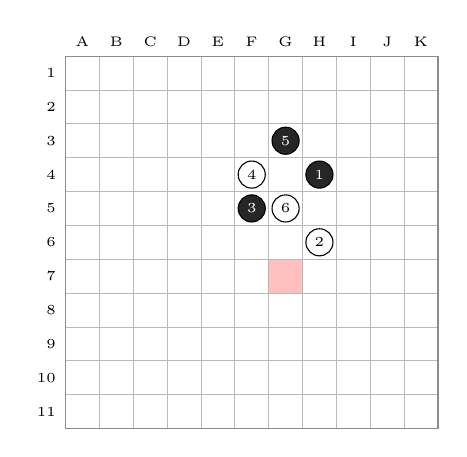
\begin{tikzpicture}[x=0.43cm, y=0.43cm]
\fill[red!25] (6,-6) rectangle (7,-7);
\draw[gray!55, line width=.3pt, step=1] (0,0) grid (11,-11);
\draw[gray!90] (0,0) rectangle (11,-11);
\node[font=\tiny, anchor=south] at (0.5,0) {A};
\node[font=\tiny, anchor=south] at (1.5,0) {B};
\node[font=\tiny, anchor=south] at (2.5,0) {C};
\node[font=\tiny, anchor=south] at (3.5,0) {D};
\node[font=\tiny, anchor=south] at (4.5,0) {E};
\node[font=\tiny, anchor=south] at (5.5,0) {F};
\node[font=\tiny, anchor=south] at (6.5,0) {G};
\node[font=\tiny, anchor=south] at (7.5,0) {H};
\node[font=\tiny, anchor=south] at (8.5,0) {I};
\node[font=\tiny, anchor=south] at (9.5,0) {J};
\node[font=\tiny, anchor=south] at (10.5,0) {K};
\node[font=\tiny, anchor=east] at (0,-0.5) {1};
\node[font=\tiny, anchor=east] at (0,-1.5) {2};
\node[font=\tiny, anchor=east] at (0,-2.5) {3};
\node[font=\tiny, anchor=east] at (0,-3.5) {4};
\node[font=\tiny, anchor=east] at (0,-4.5) {5};
\node[font=\tiny, anchor=east] at (0,-5.5) {6};
\node[font=\tiny, anchor=east] at (0,-6.5) {7};
\node[font=\tiny, anchor=east] at (0,-7.5) {8};
\node[font=\tiny, anchor=east] at (0,-8.5) {9};
\node[font=\tiny, anchor=east] at (0,-9.5) {10};
\node[font=\tiny, anchor=east] at (0,-10.5) {11};
\draw[fill=black!85, line width=.4pt] (6.5,-2.5) circle (.40);
\node[font=\tiny, text=white, inner sep=0pt] at (6.5,-2.5) {5};
\draw[fill=white, line width=.4pt] (5.5,-3.5) circle (.40);
\node[font=\tiny, text=black, inner sep=0pt] at (5.5,-3.5) {4};
\draw[fill=black!85, line width=.4pt] (7.5,-3.5) circle (.40);
\node[font=\tiny, text=white, inner sep=0pt] at (7.5,-3.5) {1};
\draw[fill=black!85, line width=.4pt] (5.5,-4.5) circle (.40);
\node[font=\tiny, text=white, inner sep=0pt] at (5.5,-4.5) {3};
\draw[fill=white, line width=.4pt] (6.5,-4.5) circle (.40);
\node[font=\tiny, text=black, inner sep=0pt] at (6.5,-4.5) {6};
\draw[fill=white, line width=.4pt] (7.5,-5.5) circle (.40);
\node[font=\tiny, text=black, inner sep=0pt] at (7.5,-5.5) {2};
\end{tikzpicture}
    \caption{Trước nước 7 (X đi; ô đỏ là nước đã chọn)}
  \end{subfigure}\hfill
  \begin{subfigure}[t]{.48\linewidth}
    \centering
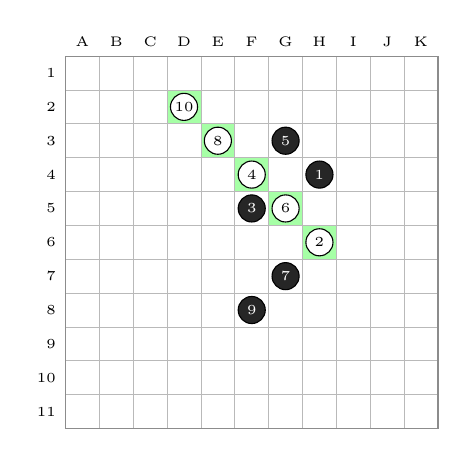
\begin{tikzpicture}[x=0.43cm, y=0.43cm]
\fill[green!35] (3,-1) rectangle (4,-2);
\fill[green!35] (4,-2) rectangle (5,-3);
\fill[green!35] (5,-3) rectangle (6,-4);
\fill[green!35] (6,-4) rectangle (7,-5);
\fill[green!35] (7,-5) rectangle (8,-6);
\draw[gray!55, line width=.3pt, step=1] (0,0) grid (11,-11);
\draw[gray!90] (0,0) rectangle (11,-11);
\node[font=\tiny, anchor=south] at (0.5,0) {A};
\node[font=\tiny, anchor=south] at (1.5,0) {B};
\node[font=\tiny, anchor=south] at (2.5,0) {C};
\node[font=\tiny, anchor=south] at (3.5,0) {D};
\node[font=\tiny, anchor=south] at (4.5,0) {E};
\node[font=\tiny, anchor=south] at (5.5,0) {F};
\node[font=\tiny, anchor=south] at (6.5,0) {G};
\node[font=\tiny, anchor=south] at (7.5,0) {H};
\node[font=\tiny, anchor=south] at (8.5,0) {I};
\node[font=\tiny, anchor=south] at (9.5,0) {J};
\node[font=\tiny, anchor=south] at (10.5,0) {K};
\node[font=\tiny, anchor=east] at (0,-0.5) {1};
\node[font=\tiny, anchor=east] at (0,-1.5) {2};
\node[font=\tiny, anchor=east] at (0,-2.5) {3};
\node[font=\tiny, anchor=east] at (0,-3.5) {4};
\node[font=\tiny, anchor=east] at (0,-4.5) {5};
\node[font=\tiny, anchor=east] at (0,-5.5) {6};
\node[font=\tiny, anchor=east] at (0,-6.5) {7};
\node[font=\tiny, anchor=east] at (0,-7.5) {8};
\node[font=\tiny, anchor=east] at (0,-8.5) {9};
\node[font=\tiny, anchor=east] at (0,-9.5) {10};
\node[font=\tiny, anchor=east] at (0,-10.5) {11};
\draw[fill=white, line width=.4pt] (3.5,-1.5) circle (.40);
\node[font=\tiny, text=black, inner sep=0pt] at (3.5,-1.5) {10};
\draw[fill=white, line width=.4pt] (4.5,-2.5) circle (.40);
\node[font=\tiny, text=black, inner sep=0pt] at (4.5,-2.5) {8};
\draw[fill=black!85, line width=.4pt] (6.5,-2.5) circle (.40);
\node[font=\tiny, text=white, inner sep=0pt] at (6.5,-2.5) {5};
\draw[fill=white, line width=.4pt] (5.5,-3.5) circle (.40);
\node[font=\tiny, text=black, inner sep=0pt] at (5.5,-3.5) {4};
\draw[fill=black!85, line width=.4pt] (7.5,-3.5) circle (.40);
\node[font=\tiny, text=white, inner sep=0pt] at (7.5,-3.5) {1};
\draw[fill=black!85, line width=.4pt] (5.5,-4.5) circle (.40);
\node[font=\tiny, text=white, inner sep=0pt] at (5.5,-4.5) {3};
\draw[fill=white, line width=.4pt] (6.5,-4.5) circle (.40);
\node[font=\tiny, text=black, inner sep=0pt] at (6.5,-4.5) {6};
\draw[fill=white, line width=.4pt] (7.5,-5.5) circle (.40);
\node[font=\tiny, text=black, inner sep=0pt] at (7.5,-5.5) {2};
\draw[fill=black!85, line width=.4pt] (6.5,-6.5) circle (.40);
\node[font=\tiny, text=white, inner sep=0pt] at (6.5,-6.5) {7};
\draw[fill=black!85, line width=.4pt] (5.5,-7.5) circle (.40);
\node[font=\tiny, text=white, inner sep=0pt] at (5.5,-7.5) {9};
\end{tikzpicture}
    \caption{Thế cuối (ô xanh: dãy thắng)}
  \end{subfigure}
  \caption{Ván 853 (L4 cầm X, L2 cầm O).}
  \label{fig:cs-van-09}
\end{figure}
{\footnotesize\linespread{1}\selectfont
\noindent\begin{tabularx}{\linewidth}{*{6}{X}}
\toprule
1.~X H4$^\ast$ & 3.~X F5$^\ast$ & 5.~X G3 & 7.~X G7 & 9.~X F8 &  \\
2.~O H6$^\ast$ & 4.~O F4$^\ast$ & 6.~O G5 & 8.~O E3 & 10.~O D2 &  \\
\bottomrule
\end{tabularx}\par}
\paragraph{Diễn biến chiến thuật.}
\begin{itemize}\small
\setlength{\itemsep}{0pt}
  \item Nước 7 (X=L4, G7): để đối thủ có VCF: E3--D2--I7.
  \item Nước 8 (O=L2, E3): đang có VCF 2 nước và đi đúng một đường (E3--D2--I7 là đường ngắn nhất).
  \item Nước 9 (X=L4, F8): đối thủ đang có các ô thắng D2, I7, không đỡ hết được.
  \item Nước 10 (O=L2, D2): thắng ngay.
\end{itemize}
Thời gian trung vị mỗi nước: X 55,8 ms, O 0,1 ms.
\clearpage

\subsection{L2 -- L5: ván 900}
\label{sec:cs-van-10}
X: \texttt{L2-Rule}; O: \texttt{L5-PolicySL}; khai cuộc 0 (3 nước, đánh dấu $\ast$); 26 nước; kết quả: O (L5) thắng. Cả cặp: L2 thắng 36, hoà 1, thua 63 trên 100 ván; trung vị 26 nước.
\begin{figure}[H]
  \centering
  \begin{subfigure}[t]{.48\linewidth}
    \centering
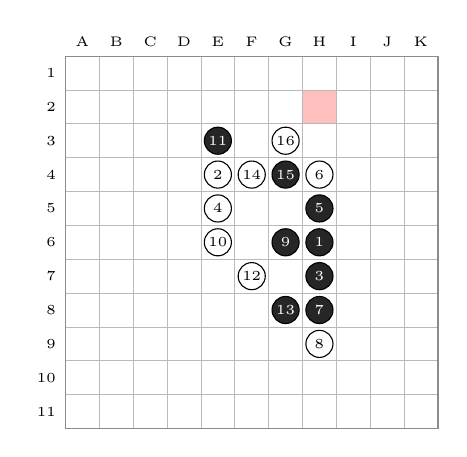
\begin{tikzpicture}[x=0.43cm, y=0.43cm]
\fill[red!25] (7,-1) rectangle (8,-2);
\draw[gray!55, line width=.3pt, step=1] (0,0) grid (11,-11);
\draw[gray!90] (0,0) rectangle (11,-11);
\node[font=\tiny, anchor=south] at (0.5,0) {A};
\node[font=\tiny, anchor=south] at (1.5,0) {B};
\node[font=\tiny, anchor=south] at (2.5,0) {C};
\node[font=\tiny, anchor=south] at (3.5,0) {D};
\node[font=\tiny, anchor=south] at (4.5,0) {E};
\node[font=\tiny, anchor=south] at (5.5,0) {F};
\node[font=\tiny, anchor=south] at (6.5,0) {G};
\node[font=\tiny, anchor=south] at (7.5,0) {H};
\node[font=\tiny, anchor=south] at (8.5,0) {I};
\node[font=\tiny, anchor=south] at (9.5,0) {J};
\node[font=\tiny, anchor=south] at (10.5,0) {K};
\node[font=\tiny, anchor=east] at (0,-0.5) {1};
\node[font=\tiny, anchor=east] at (0,-1.5) {2};
\node[font=\tiny, anchor=east] at (0,-2.5) {3};
\node[font=\tiny, anchor=east] at (0,-3.5) {4};
\node[font=\tiny, anchor=east] at (0,-4.5) {5};
\node[font=\tiny, anchor=east] at (0,-5.5) {6};
\node[font=\tiny, anchor=east] at (0,-6.5) {7};
\node[font=\tiny, anchor=east] at (0,-7.5) {8};
\node[font=\tiny, anchor=east] at (0,-8.5) {9};
\node[font=\tiny, anchor=east] at (0,-9.5) {10};
\node[font=\tiny, anchor=east] at (0,-10.5) {11};
\draw[fill=black!85, line width=.4pt] (4.5,-2.5) circle (.40);
\node[font=\tiny, text=white, inner sep=0pt] at (4.5,-2.5) {11};
\draw[fill=white, line width=.4pt] (6.5,-2.5) circle (.40);
\node[font=\tiny, text=black, inner sep=0pt] at (6.5,-2.5) {16};
\draw[fill=white, line width=.4pt] (4.5,-3.5) circle (.40);
\node[font=\tiny, text=black, inner sep=0pt] at (4.5,-3.5) {2};
\draw[fill=white, line width=.4pt] (5.5,-3.5) circle (.40);
\node[font=\tiny, text=black, inner sep=0pt] at (5.5,-3.5) {14};
\draw[fill=black!85, line width=.4pt] (6.5,-3.5) circle (.40);
\node[font=\tiny, text=white, inner sep=0pt] at (6.5,-3.5) {15};
\draw[fill=white, line width=.4pt] (7.5,-3.5) circle (.40);
\node[font=\tiny, text=black, inner sep=0pt] at (7.5,-3.5) {6};
\draw[fill=white, line width=.4pt] (4.5,-4.5) circle (.40);
\node[font=\tiny, text=black, inner sep=0pt] at (4.5,-4.5) {4};
\draw[fill=black!85, line width=.4pt] (7.5,-4.5) circle (.40);
\node[font=\tiny, text=white, inner sep=0pt] at (7.5,-4.5) {5};
\draw[fill=white, line width=.4pt] (4.5,-5.5) circle (.40);
\node[font=\tiny, text=black, inner sep=0pt] at (4.5,-5.5) {10};
\draw[fill=black!85, line width=.4pt] (6.5,-5.5) circle (.40);
\node[font=\tiny, text=white, inner sep=0pt] at (6.5,-5.5) {9};
\draw[fill=black!85, line width=.4pt] (7.5,-5.5) circle (.40);
\node[font=\tiny, text=white, inner sep=0pt] at (7.5,-5.5) {1};
\draw[fill=white, line width=.4pt] (5.5,-6.5) circle (.40);
\node[font=\tiny, text=black, inner sep=0pt] at (5.5,-6.5) {12};
\draw[fill=black!85, line width=.4pt] (7.5,-6.5) circle (.40);
\node[font=\tiny, text=white, inner sep=0pt] at (7.5,-6.5) {3};
\draw[fill=black!85, line width=.4pt] (6.5,-7.5) circle (.40);
\node[font=\tiny, text=white, inner sep=0pt] at (6.5,-7.5) {13};
\draw[fill=black!85, line width=.4pt] (7.5,-7.5) circle (.40);
\node[font=\tiny, text=white, inner sep=0pt] at (7.5,-7.5) {7};
\draw[fill=white, line width=.4pt] (7.5,-8.5) circle (.40);
\node[font=\tiny, text=black, inner sep=0pt] at (7.5,-8.5) {8};
\end{tikzpicture}
    \caption{Trước nước 17 (X đi; ô đỏ là nước đã chọn)}
  \end{subfigure}\hfill
  \begin{subfigure}[t]{.48\linewidth}
    \centering
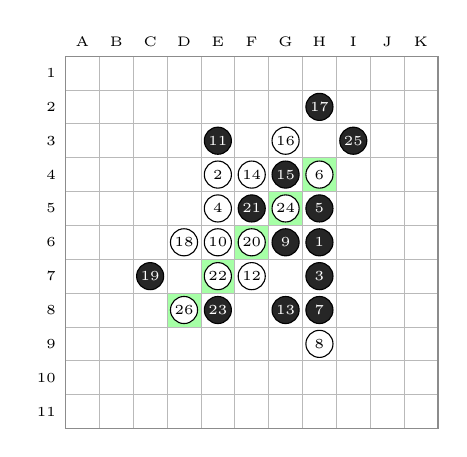
\begin{tikzpicture}[x=0.43cm, y=0.43cm]
\fill[green!35] (3,-7) rectangle (4,-8);
\fill[green!35] (4,-6) rectangle (5,-7);
\fill[green!35] (5,-5) rectangle (6,-6);
\fill[green!35] (6,-4) rectangle (7,-5);
\fill[green!35] (7,-3) rectangle (8,-4);
\draw[gray!55, line width=.3pt, step=1] (0,0) grid (11,-11);
\draw[gray!90] (0,0) rectangle (11,-11);
\node[font=\tiny, anchor=south] at (0.5,0) {A};
\node[font=\tiny, anchor=south] at (1.5,0) {B};
\node[font=\tiny, anchor=south] at (2.5,0) {C};
\node[font=\tiny, anchor=south] at (3.5,0) {D};
\node[font=\tiny, anchor=south] at (4.5,0) {E};
\node[font=\tiny, anchor=south] at (5.5,0) {F};
\node[font=\tiny, anchor=south] at (6.5,0) {G};
\node[font=\tiny, anchor=south] at (7.5,0) {H};
\node[font=\tiny, anchor=south] at (8.5,0) {I};
\node[font=\tiny, anchor=south] at (9.5,0) {J};
\node[font=\tiny, anchor=south] at (10.5,0) {K};
\node[font=\tiny, anchor=east] at (0,-0.5) {1};
\node[font=\tiny, anchor=east] at (0,-1.5) {2};
\node[font=\tiny, anchor=east] at (0,-2.5) {3};
\node[font=\tiny, anchor=east] at (0,-3.5) {4};
\node[font=\tiny, anchor=east] at (0,-4.5) {5};
\node[font=\tiny, anchor=east] at (0,-5.5) {6};
\node[font=\tiny, anchor=east] at (0,-6.5) {7};
\node[font=\tiny, anchor=east] at (0,-7.5) {8};
\node[font=\tiny, anchor=east] at (0,-8.5) {9};
\node[font=\tiny, anchor=east] at (0,-9.5) {10};
\node[font=\tiny, anchor=east] at (0,-10.5) {11};
\draw[fill=black!85, line width=.4pt] (7.5,-1.5) circle (.40);
\node[font=\tiny, text=white, inner sep=0pt] at (7.5,-1.5) {17};
\draw[fill=black!85, line width=.4pt] (4.5,-2.5) circle (.40);
\node[font=\tiny, text=white, inner sep=0pt] at (4.5,-2.5) {11};
\draw[fill=white, line width=.4pt] (6.5,-2.5) circle (.40);
\node[font=\tiny, text=black, inner sep=0pt] at (6.5,-2.5) {16};
\draw[fill=black!85, line width=.4pt] (8.5,-2.5) circle (.40);
\node[font=\tiny, text=white, inner sep=0pt] at (8.5,-2.5) {25};
\draw[fill=white, line width=.4pt] (4.5,-3.5) circle (.40);
\node[font=\tiny, text=black, inner sep=0pt] at (4.5,-3.5) {2};
\draw[fill=white, line width=.4pt] (5.5,-3.5) circle (.40);
\node[font=\tiny, text=black, inner sep=0pt] at (5.5,-3.5) {14};
\draw[fill=black!85, line width=.4pt] (6.5,-3.5) circle (.40);
\node[font=\tiny, text=white, inner sep=0pt] at (6.5,-3.5) {15};
\draw[fill=white, line width=.4pt] (7.5,-3.5) circle (.40);
\node[font=\tiny, text=black, inner sep=0pt] at (7.5,-3.5) {6};
\draw[fill=white, line width=.4pt] (4.5,-4.5) circle (.40);
\node[font=\tiny, text=black, inner sep=0pt] at (4.5,-4.5) {4};
\draw[fill=black!85, line width=.4pt] (5.5,-4.5) circle (.40);
\node[font=\tiny, text=white, inner sep=0pt] at (5.5,-4.5) {21};
\draw[fill=white, line width=.4pt] (6.5,-4.5) circle (.40);
\node[font=\tiny, text=black, inner sep=0pt] at (6.5,-4.5) {24};
\draw[fill=black!85, line width=.4pt] (7.5,-4.5) circle (.40);
\node[font=\tiny, text=white, inner sep=0pt] at (7.5,-4.5) {5};
\draw[fill=white, line width=.4pt] (3.5,-5.5) circle (.40);
\node[font=\tiny, text=black, inner sep=0pt] at (3.5,-5.5) {18};
\draw[fill=white, line width=.4pt] (4.5,-5.5) circle (.40);
\node[font=\tiny, text=black, inner sep=0pt] at (4.5,-5.5) {10};
\draw[fill=white, line width=.4pt] (5.5,-5.5) circle (.40);
\node[font=\tiny, text=black, inner sep=0pt] at (5.5,-5.5) {20};
\draw[fill=black!85, line width=.4pt] (6.5,-5.5) circle (.40);
\node[font=\tiny, text=white, inner sep=0pt] at (6.5,-5.5) {9};
\draw[fill=black!85, line width=.4pt] (7.5,-5.5) circle (.40);
\node[font=\tiny, text=white, inner sep=0pt] at (7.5,-5.5) {1};
\draw[fill=black!85, line width=.4pt] (2.5,-6.5) circle (.40);
\node[font=\tiny, text=white, inner sep=0pt] at (2.5,-6.5) {19};
\draw[fill=white, line width=.4pt] (4.5,-6.5) circle (.40);
\node[font=\tiny, text=black, inner sep=0pt] at (4.5,-6.5) {22};
\draw[fill=white, line width=.4pt] (5.5,-6.5) circle (.40);
\node[font=\tiny, text=black, inner sep=0pt] at (5.5,-6.5) {12};
\draw[fill=black!85, line width=.4pt] (7.5,-6.5) circle (.40);
\node[font=\tiny, text=white, inner sep=0pt] at (7.5,-6.5) {3};
\draw[fill=white, line width=.4pt] (3.5,-7.5) circle (.40);
\node[font=\tiny, text=black, inner sep=0pt] at (3.5,-7.5) {26};
\draw[fill=black!85, line width=.4pt] (4.5,-7.5) circle (.40);
\node[font=\tiny, text=white, inner sep=0pt] at (4.5,-7.5) {23};
\draw[fill=black!85, line width=.4pt] (6.5,-7.5) circle (.40);
\node[font=\tiny, text=white, inner sep=0pt] at (6.5,-7.5) {13};
\draw[fill=black!85, line width=.4pt] (7.5,-7.5) circle (.40);
\node[font=\tiny, text=white, inner sep=0pt] at (7.5,-7.5) {7};
\draw[fill=white, line width=.4pt] (7.5,-8.5) circle (.40);
\node[font=\tiny, text=black, inner sep=0pt] at (7.5,-8.5) {8};
\end{tikzpicture}
    \caption{Thế cuối (ô xanh: dãy thắng)}
  \end{subfigure}
  \caption{Ván 900 (L2 cầm X, L5 cầm O).}
  \label{fig:cs-van-10}
\end{figure}
{\footnotesize\linespread{1}\selectfont
\noindent\begin{tabularx}{\linewidth}{*{6}{X}}
\toprule
1.~X H6$^\ast$ & 6.~O H4 & 11.~X E3 & 16.~O G3 & 21.~X F5 & 26.~O D8 \\
2.~O E4$^\ast$ & 7.~X H8 & 12.~O F7 & 17.~X H2 & 22.~O E7 &  \\
3.~X H7$^\ast$ & 8.~O H9 & 13.~X G8 & 18.~O D6 & 23.~X E8 &  \\
4.~O E5 & 9.~X G6 & 14.~O F4 & 19.~X C7 & 24.~O G5 &  \\
5.~X H5 & 10.~O E6 & 15.~X G4 & 20.~O F6 & 25.~X I3 &  \\
\bottomrule
\end{tabularx}\par}
\paragraph{Diễn biến chiến thuật.}
\begin{itemize}\small
\setlength{\itemsep}{0pt}
  \item Nước 8 (O=L5, H9): chặn ô thắng H9.
  \item Nước 17 (X=L2, H2): để đối thủ có VCF: C7--D6--E7--E8--D7--B7--G7.
  \item Nước 18 (O=L5, D6): bỏ lỡ VCF 4 nước: C7--D6--E7--E8--D7--B7--G7.
  \item Nước 19 (X=L2, C7): chặn ô thắng C7.
  \item Nước 21 (X=L2, F5): để đối thủ có VCF: E7--E8--G5--I3--D8.
  \item Nước 22 (O=L5, E7): đang có VCF 3 nước và đi đúng một đường (E7--E8--G5--I3--D8 là đường ngắn nhất).
  \item Nước 23 (X=L2, E8): chặn ô thắng E8.
  \item Nước 24 (O=L5, G5): đang có VCF 2 nước và đi đúng một đường (G5--I3--D8 là đường ngắn nhất).
  \item Nước 25 (X=L2, I3): đối thủ đang có các ô thắng I3, D8, không đỡ hết được.
  \item Nước 26 (O=L5, D8): thắng ngay.
\end{itemize}
Thời gian trung vị mỗi nước: X 0,8 ms, O 0,9 ms.
\clearpage

\subsection{L2 -- L6: ván 1070}
\label{sec:cs-van-11}
X: \texttt{L2-Rule}; O: \texttt{L6-PolicyRL}; khai cuộc 35 (2 nước, đánh dấu $\ast$); 24 nước; kết quả: O (L6) thắng. Cả cặp: L2 thắng 30, hoà 4, thua 66 trên 100 ván; trung vị 24 nước.
\begin{figure}[H]
  \centering
  \begin{subfigure}[t]{.48\linewidth}
    \centering
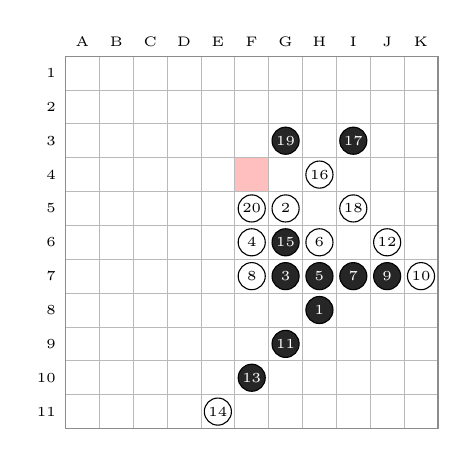
\begin{tikzpicture}[x=0.43cm, y=0.43cm]
\fill[red!25] (5,-3) rectangle (6,-4);
\draw[gray!55, line width=.3pt, step=1] (0,0) grid (11,-11);
\draw[gray!90] (0,0) rectangle (11,-11);
\node[font=\tiny, anchor=south] at (0.5,0) {A};
\node[font=\tiny, anchor=south] at (1.5,0) {B};
\node[font=\tiny, anchor=south] at (2.5,0) {C};
\node[font=\tiny, anchor=south] at (3.5,0) {D};
\node[font=\tiny, anchor=south] at (4.5,0) {E};
\node[font=\tiny, anchor=south] at (5.5,0) {F};
\node[font=\tiny, anchor=south] at (6.5,0) {G};
\node[font=\tiny, anchor=south] at (7.5,0) {H};
\node[font=\tiny, anchor=south] at (8.5,0) {I};
\node[font=\tiny, anchor=south] at (9.5,0) {J};
\node[font=\tiny, anchor=south] at (10.5,0) {K};
\node[font=\tiny, anchor=east] at (0,-0.5) {1};
\node[font=\tiny, anchor=east] at (0,-1.5) {2};
\node[font=\tiny, anchor=east] at (0,-2.5) {3};
\node[font=\tiny, anchor=east] at (0,-3.5) {4};
\node[font=\tiny, anchor=east] at (0,-4.5) {5};
\node[font=\tiny, anchor=east] at (0,-5.5) {6};
\node[font=\tiny, anchor=east] at (0,-6.5) {7};
\node[font=\tiny, anchor=east] at (0,-7.5) {8};
\node[font=\tiny, anchor=east] at (0,-8.5) {9};
\node[font=\tiny, anchor=east] at (0,-9.5) {10};
\node[font=\tiny, anchor=east] at (0,-10.5) {11};
\draw[fill=black!85, line width=.4pt] (6.5,-2.5) circle (.40);
\node[font=\tiny, text=white, inner sep=0pt] at (6.5,-2.5) {19};
\draw[fill=black!85, line width=.4pt] (8.5,-2.5) circle (.40);
\node[font=\tiny, text=white, inner sep=0pt] at (8.5,-2.5) {17};
\draw[fill=white, line width=.4pt] (7.5,-3.5) circle (.40);
\node[font=\tiny, text=black, inner sep=0pt] at (7.5,-3.5) {16};
\draw[fill=white, line width=.4pt] (5.5,-4.5) circle (.40);
\node[font=\tiny, text=black, inner sep=0pt] at (5.5,-4.5) {20};
\draw[fill=white, line width=.4pt] (6.5,-4.5) circle (.40);
\node[font=\tiny, text=black, inner sep=0pt] at (6.5,-4.5) {2};
\draw[fill=white, line width=.4pt] (8.5,-4.5) circle (.40);
\node[font=\tiny, text=black, inner sep=0pt] at (8.5,-4.5) {18};
\draw[fill=white, line width=.4pt] (5.5,-5.5) circle (.40);
\node[font=\tiny, text=black, inner sep=0pt] at (5.5,-5.5) {4};
\draw[fill=black!85, line width=.4pt] (6.5,-5.5) circle (.40);
\node[font=\tiny, text=white, inner sep=0pt] at (6.5,-5.5) {15};
\draw[fill=white, line width=.4pt] (7.5,-5.5) circle (.40);
\node[font=\tiny, text=black, inner sep=0pt] at (7.5,-5.5) {6};
\draw[fill=white, line width=.4pt] (9.5,-5.5) circle (.40);
\node[font=\tiny, text=black, inner sep=0pt] at (9.5,-5.5) {12};
\draw[fill=white, line width=.4pt] (5.5,-6.5) circle (.40);
\node[font=\tiny, text=black, inner sep=0pt] at (5.5,-6.5) {8};
\draw[fill=black!85, line width=.4pt] (6.5,-6.5) circle (.40);
\node[font=\tiny, text=white, inner sep=0pt] at (6.5,-6.5) {3};
\draw[fill=black!85, line width=.4pt] (7.5,-6.5) circle (.40);
\node[font=\tiny, text=white, inner sep=0pt] at (7.5,-6.5) {5};
\draw[fill=black!85, line width=.4pt] (8.5,-6.5) circle (.40);
\node[font=\tiny, text=white, inner sep=0pt] at (8.5,-6.5) {7};
\draw[fill=black!85, line width=.4pt] (9.5,-6.5) circle (.40);
\node[font=\tiny, text=white, inner sep=0pt] at (9.5,-6.5) {9};
\draw[fill=white, line width=.4pt] (10.5,-6.5) circle (.40);
\node[font=\tiny, text=black, inner sep=0pt] at (10.5,-6.5) {10};
\draw[fill=black!85, line width=.4pt] (7.5,-7.5) circle (.40);
\node[font=\tiny, text=white, inner sep=0pt] at (7.5,-7.5) {1};
\draw[fill=black!85, line width=.4pt] (6.5,-8.5) circle (.40);
\node[font=\tiny, text=white, inner sep=0pt] at (6.5,-8.5) {11};
\draw[fill=black!85, line width=.4pt] (5.5,-9.5) circle (.40);
\node[font=\tiny, text=white, inner sep=0pt] at (5.5,-9.5) {13};
\draw[fill=white, line width=.4pt] (4.5,-10.5) circle (.40);
\node[font=\tiny, text=black, inner sep=0pt] at (4.5,-10.5) {14};
\end{tikzpicture}
    \caption{Trước nước 21 (X đi; ô đỏ là nước đã chọn)}
  \end{subfigure}\hfill
  \begin{subfigure}[t]{.48\linewidth}
    \centering
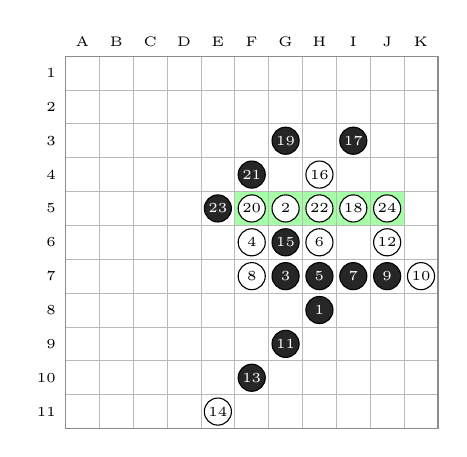
\begin{tikzpicture}[x=0.43cm, y=0.43cm]
\fill[green!35] (9,-4) rectangle (10,-5);
\fill[green!35] (8,-4) rectangle (9,-5);
\fill[green!35] (7,-4) rectangle (8,-5);
\fill[green!35] (6,-4) rectangle (7,-5);
\fill[green!35] (5,-4) rectangle (6,-5);
\draw[gray!55, line width=.3pt, step=1] (0,0) grid (11,-11);
\draw[gray!90] (0,0) rectangle (11,-11);
\node[font=\tiny, anchor=south] at (0.5,0) {A};
\node[font=\tiny, anchor=south] at (1.5,0) {B};
\node[font=\tiny, anchor=south] at (2.5,0) {C};
\node[font=\tiny, anchor=south] at (3.5,0) {D};
\node[font=\tiny, anchor=south] at (4.5,0) {E};
\node[font=\tiny, anchor=south] at (5.5,0) {F};
\node[font=\tiny, anchor=south] at (6.5,0) {G};
\node[font=\tiny, anchor=south] at (7.5,0) {H};
\node[font=\tiny, anchor=south] at (8.5,0) {I};
\node[font=\tiny, anchor=south] at (9.5,0) {J};
\node[font=\tiny, anchor=south] at (10.5,0) {K};
\node[font=\tiny, anchor=east] at (0,-0.5) {1};
\node[font=\tiny, anchor=east] at (0,-1.5) {2};
\node[font=\tiny, anchor=east] at (0,-2.5) {3};
\node[font=\tiny, anchor=east] at (0,-3.5) {4};
\node[font=\tiny, anchor=east] at (0,-4.5) {5};
\node[font=\tiny, anchor=east] at (0,-5.5) {6};
\node[font=\tiny, anchor=east] at (0,-6.5) {7};
\node[font=\tiny, anchor=east] at (0,-7.5) {8};
\node[font=\tiny, anchor=east] at (0,-8.5) {9};
\node[font=\tiny, anchor=east] at (0,-9.5) {10};
\node[font=\tiny, anchor=east] at (0,-10.5) {11};
\draw[fill=black!85, line width=.4pt] (6.5,-2.5) circle (.40);
\node[font=\tiny, text=white, inner sep=0pt] at (6.5,-2.5) {19};
\draw[fill=black!85, line width=.4pt] (8.5,-2.5) circle (.40);
\node[font=\tiny, text=white, inner sep=0pt] at (8.5,-2.5) {17};
\draw[fill=black!85, line width=.4pt] (5.5,-3.5) circle (.40);
\node[font=\tiny, text=white, inner sep=0pt] at (5.5,-3.5) {21};
\draw[fill=white, line width=.4pt] (7.5,-3.5) circle (.40);
\node[font=\tiny, text=black, inner sep=0pt] at (7.5,-3.5) {16};
\draw[fill=black!85, line width=.4pt] (4.5,-4.5) circle (.40);
\node[font=\tiny, text=white, inner sep=0pt] at (4.5,-4.5) {23};
\draw[fill=white, line width=.4pt] (5.5,-4.5) circle (.40);
\node[font=\tiny, text=black, inner sep=0pt] at (5.5,-4.5) {20};
\draw[fill=white, line width=.4pt] (6.5,-4.5) circle (.40);
\node[font=\tiny, text=black, inner sep=0pt] at (6.5,-4.5) {2};
\draw[fill=white, line width=.4pt] (7.5,-4.5) circle (.40);
\node[font=\tiny, text=black, inner sep=0pt] at (7.5,-4.5) {22};
\draw[fill=white, line width=.4pt] (8.5,-4.5) circle (.40);
\node[font=\tiny, text=black, inner sep=0pt] at (8.5,-4.5) {18};
\draw[fill=white, line width=.4pt] (9.5,-4.5) circle (.40);
\node[font=\tiny, text=black, inner sep=0pt] at (9.5,-4.5) {24};
\draw[fill=white, line width=.4pt] (5.5,-5.5) circle (.40);
\node[font=\tiny, text=black, inner sep=0pt] at (5.5,-5.5) {4};
\draw[fill=black!85, line width=.4pt] (6.5,-5.5) circle (.40);
\node[font=\tiny, text=white, inner sep=0pt] at (6.5,-5.5) {15};
\draw[fill=white, line width=.4pt] (7.5,-5.5) circle (.40);
\node[font=\tiny, text=black, inner sep=0pt] at (7.5,-5.5) {6};
\draw[fill=white, line width=.4pt] (9.5,-5.5) circle (.40);
\node[font=\tiny, text=black, inner sep=0pt] at (9.5,-5.5) {12};
\draw[fill=white, line width=.4pt] (5.5,-6.5) circle (.40);
\node[font=\tiny, text=black, inner sep=0pt] at (5.5,-6.5) {8};
\draw[fill=black!85, line width=.4pt] (6.5,-6.5) circle (.40);
\node[font=\tiny, text=white, inner sep=0pt] at (6.5,-6.5) {3};
\draw[fill=black!85, line width=.4pt] (7.5,-6.5) circle (.40);
\node[font=\tiny, text=white, inner sep=0pt] at (7.5,-6.5) {5};
\draw[fill=black!85, line width=.4pt] (8.5,-6.5) circle (.40);
\node[font=\tiny, text=white, inner sep=0pt] at (8.5,-6.5) {7};
\draw[fill=black!85, line width=.4pt] (9.5,-6.5) circle (.40);
\node[font=\tiny, text=white, inner sep=0pt] at (9.5,-6.5) {9};
\draw[fill=white, line width=.4pt] (10.5,-6.5) circle (.40);
\node[font=\tiny, text=black, inner sep=0pt] at (10.5,-6.5) {10};
\draw[fill=black!85, line width=.4pt] (7.5,-7.5) circle (.40);
\node[font=\tiny, text=white, inner sep=0pt] at (7.5,-7.5) {1};
\draw[fill=black!85, line width=.4pt] (6.5,-8.5) circle (.40);
\node[font=\tiny, text=white, inner sep=0pt] at (6.5,-8.5) {11};
\draw[fill=black!85, line width=.4pt] (5.5,-9.5) circle (.40);
\node[font=\tiny, text=white, inner sep=0pt] at (5.5,-9.5) {13};
\draw[fill=white, line width=.4pt] (4.5,-10.5) circle (.40);
\node[font=\tiny, text=black, inner sep=0pt] at (4.5,-10.5) {14};
\end{tikzpicture}
    \caption{Thế cuối (ô xanh: dãy thắng)}
  \end{subfigure}
  \caption{Ván 1070 (L2 cầm X, L6 cầm O).}
  \label{fig:cs-van-11}
\end{figure}
{\footnotesize\linespread{1}\selectfont
\noindent\begin{tabularx}{\linewidth}{*{6}{X}}
\toprule
1.~X H8$^\ast$ & 5.~X H7 & 9.~X J7 & 13.~X F10 & 17.~X I3 & 21.~X F4 \\
2.~O G5$^\ast$ & 6.~O H6 & 10.~O K7 & 14.~O E11 & 18.~O I5 & 22.~O H5 \\
3.~X G7 & 7.~X I7 & 11.~X G9 & 15.~X G6 & 19.~X G3 & 23.~X E5 \\
4.~O F6 & 8.~O F7 & 12.~O J6 & 16.~O H4 & 20.~O F5 & 24.~O J5 \\
\bottomrule
\end{tabularx}\par}
\paragraph{Diễn biến chiến thuật.}
\begin{itemize}\small
\setlength{\itemsep}{0pt}
  \item Nước 10 (O=L6, K7): chặn ô thắng K7.
  \item Nước 14 (O=L6, E11): chặn ô thắng E11.
  \item Nước 19 (X=L2, G3): chặn ô thắng G3.
  \item Nước 21 (X=L2, F4): để đối thủ có VCF: H5--E5--J5.
  \item Nước 22 (O=L6, H5): đang có VCF 2 nước và đi đúng một đường (H5--E5--J5 là đường ngắn nhất).
  \item Nước 23 (X=L2, E5): đối thủ đang có các ô thắng E5, J5, không đỡ hết được.
  \item Nước 24 (O=L6, J5): thắng ngay.
\end{itemize}
Thời gian trung vị mỗi nước: X 1,4 ms, O 0,9 ms.
\clearpage

\subsection{L2 -- L7: ván 1112}
\label{sec:cs-van-12}
X: \texttt{L2-Rule}; O: \texttt{L7-PUCT}; khai cuộc 6 (3 nước, đánh dấu $\ast$); 24 nước; kết quả: O (L7) thắng. Cả cặp: L2 thắng 9, hoà 0, thua 91 trên 100 ván; trung vị 24 nước.
\begin{figure}[H]
  \centering
  \begin{subfigure}[t]{.48\linewidth}
    \centering
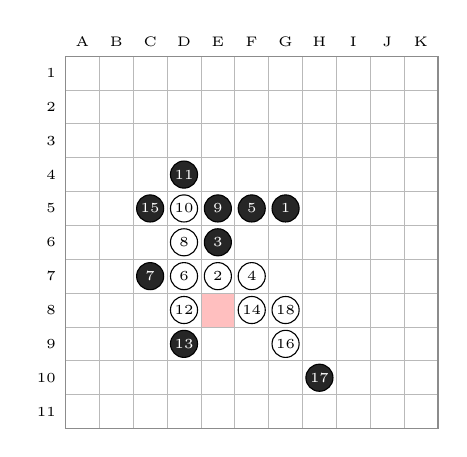
\begin{tikzpicture}[x=0.43cm, y=0.43cm]
\fill[red!25] (4,-7) rectangle (5,-8);
\draw[gray!55, line width=.3pt, step=1] (0,0) grid (11,-11);
\draw[gray!90] (0,0) rectangle (11,-11);
\node[font=\tiny, anchor=south] at (0.5,0) {A};
\node[font=\tiny, anchor=south] at (1.5,0) {B};
\node[font=\tiny, anchor=south] at (2.5,0) {C};
\node[font=\tiny, anchor=south] at (3.5,0) {D};
\node[font=\tiny, anchor=south] at (4.5,0) {E};
\node[font=\tiny, anchor=south] at (5.5,0) {F};
\node[font=\tiny, anchor=south] at (6.5,0) {G};
\node[font=\tiny, anchor=south] at (7.5,0) {H};
\node[font=\tiny, anchor=south] at (8.5,0) {I};
\node[font=\tiny, anchor=south] at (9.5,0) {J};
\node[font=\tiny, anchor=south] at (10.5,0) {K};
\node[font=\tiny, anchor=east] at (0,-0.5) {1};
\node[font=\tiny, anchor=east] at (0,-1.5) {2};
\node[font=\tiny, anchor=east] at (0,-2.5) {3};
\node[font=\tiny, anchor=east] at (0,-3.5) {4};
\node[font=\tiny, anchor=east] at (0,-4.5) {5};
\node[font=\tiny, anchor=east] at (0,-5.5) {6};
\node[font=\tiny, anchor=east] at (0,-6.5) {7};
\node[font=\tiny, anchor=east] at (0,-7.5) {8};
\node[font=\tiny, anchor=east] at (0,-8.5) {9};
\node[font=\tiny, anchor=east] at (0,-9.5) {10};
\node[font=\tiny, anchor=east] at (0,-10.5) {11};
\draw[fill=black!85, line width=.4pt] (3.5,-3.5) circle (.40);
\node[font=\tiny, text=white, inner sep=0pt] at (3.5,-3.5) {11};
\draw[fill=black!85, line width=.4pt] (2.5,-4.5) circle (.40);
\node[font=\tiny, text=white, inner sep=0pt] at (2.5,-4.5) {15};
\draw[fill=white, line width=.4pt] (3.5,-4.5) circle (.40);
\node[font=\tiny, text=black, inner sep=0pt] at (3.5,-4.5) {10};
\draw[fill=black!85, line width=.4pt] (4.5,-4.5) circle (.40);
\node[font=\tiny, text=white, inner sep=0pt] at (4.5,-4.5) {9};
\draw[fill=black!85, line width=.4pt] (5.5,-4.5) circle (.40);
\node[font=\tiny, text=white, inner sep=0pt] at (5.5,-4.5) {5};
\draw[fill=black!85, line width=.4pt] (6.5,-4.5) circle (.40);
\node[font=\tiny, text=white, inner sep=0pt] at (6.5,-4.5) {1};
\draw[fill=white, line width=.4pt] (3.5,-5.5) circle (.40);
\node[font=\tiny, text=black, inner sep=0pt] at (3.5,-5.5) {8};
\draw[fill=black!85, line width=.4pt] (4.5,-5.5) circle (.40);
\node[font=\tiny, text=white, inner sep=0pt] at (4.5,-5.5) {3};
\draw[fill=black!85, line width=.4pt] (2.5,-6.5) circle (.40);
\node[font=\tiny, text=white, inner sep=0pt] at (2.5,-6.5) {7};
\draw[fill=white, line width=.4pt] (3.5,-6.5) circle (.40);
\node[font=\tiny, text=black, inner sep=0pt] at (3.5,-6.5) {6};
\draw[fill=white, line width=.4pt] (4.5,-6.5) circle (.40);
\node[font=\tiny, text=black, inner sep=0pt] at (4.5,-6.5) {2};
\draw[fill=white, line width=.4pt] (5.5,-6.5) circle (.40);
\node[font=\tiny, text=black, inner sep=0pt] at (5.5,-6.5) {4};
\draw[fill=white, line width=.4pt] (3.5,-7.5) circle (.40);
\node[font=\tiny, text=black, inner sep=0pt] at (3.5,-7.5) {12};
\draw[fill=white, line width=.4pt] (5.5,-7.5) circle (.40);
\node[font=\tiny, text=black, inner sep=0pt] at (5.5,-7.5) {14};
\draw[fill=white, line width=.4pt] (6.5,-7.5) circle (.40);
\node[font=\tiny, text=black, inner sep=0pt] at (6.5,-7.5) {18};
\draw[fill=black!85, line width=.4pt] (3.5,-8.5) circle (.40);
\node[font=\tiny, text=white, inner sep=0pt] at (3.5,-8.5) {13};
\draw[fill=white, line width=.4pt] (6.5,-8.5) circle (.40);
\node[font=\tiny, text=black, inner sep=0pt] at (6.5,-8.5) {16};
\draw[fill=black!85, line width=.4pt] (7.5,-9.5) circle (.40);
\node[font=\tiny, text=white, inner sep=0pt] at (7.5,-9.5) {17};
\end{tikzpicture}
    \caption{Trước nước 19 (X đi; ô đỏ là nước đã chọn)}
  \end{subfigure}\hfill
  \begin{subfigure}[t]{.48\linewidth}
    \centering
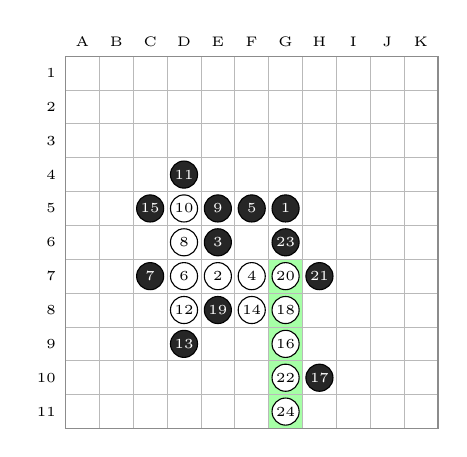
\begin{tikzpicture}[x=0.43cm, y=0.43cm]
\fill[green!35] (6,-10) rectangle (7,-11);
\fill[green!35] (6,-9) rectangle (7,-10);
\fill[green!35] (6,-8) rectangle (7,-9);
\fill[green!35] (6,-7) rectangle (7,-8);
\fill[green!35] (6,-6) rectangle (7,-7);
\draw[gray!55, line width=.3pt, step=1] (0,0) grid (11,-11);
\draw[gray!90] (0,0) rectangle (11,-11);
\node[font=\tiny, anchor=south] at (0.5,0) {A};
\node[font=\tiny, anchor=south] at (1.5,0) {B};
\node[font=\tiny, anchor=south] at (2.5,0) {C};
\node[font=\tiny, anchor=south] at (3.5,0) {D};
\node[font=\tiny, anchor=south] at (4.5,0) {E};
\node[font=\tiny, anchor=south] at (5.5,0) {F};
\node[font=\tiny, anchor=south] at (6.5,0) {G};
\node[font=\tiny, anchor=south] at (7.5,0) {H};
\node[font=\tiny, anchor=south] at (8.5,0) {I};
\node[font=\tiny, anchor=south] at (9.5,0) {J};
\node[font=\tiny, anchor=south] at (10.5,0) {K};
\node[font=\tiny, anchor=east] at (0,-0.5) {1};
\node[font=\tiny, anchor=east] at (0,-1.5) {2};
\node[font=\tiny, anchor=east] at (0,-2.5) {3};
\node[font=\tiny, anchor=east] at (0,-3.5) {4};
\node[font=\tiny, anchor=east] at (0,-4.5) {5};
\node[font=\tiny, anchor=east] at (0,-5.5) {6};
\node[font=\tiny, anchor=east] at (0,-6.5) {7};
\node[font=\tiny, anchor=east] at (0,-7.5) {8};
\node[font=\tiny, anchor=east] at (0,-8.5) {9};
\node[font=\tiny, anchor=east] at (0,-9.5) {10};
\node[font=\tiny, anchor=east] at (0,-10.5) {11};
\draw[fill=black!85, line width=.4pt] (3.5,-3.5) circle (.40);
\node[font=\tiny, text=white, inner sep=0pt] at (3.5,-3.5) {11};
\draw[fill=black!85, line width=.4pt] (2.5,-4.5) circle (.40);
\node[font=\tiny, text=white, inner sep=0pt] at (2.5,-4.5) {15};
\draw[fill=white, line width=.4pt] (3.5,-4.5) circle (.40);
\node[font=\tiny, text=black, inner sep=0pt] at (3.5,-4.5) {10};
\draw[fill=black!85, line width=.4pt] (4.5,-4.5) circle (.40);
\node[font=\tiny, text=white, inner sep=0pt] at (4.5,-4.5) {9};
\draw[fill=black!85, line width=.4pt] (5.5,-4.5) circle (.40);
\node[font=\tiny, text=white, inner sep=0pt] at (5.5,-4.5) {5};
\draw[fill=black!85, line width=.4pt] (6.5,-4.5) circle (.40);
\node[font=\tiny, text=white, inner sep=0pt] at (6.5,-4.5) {1};
\draw[fill=white, line width=.4pt] (3.5,-5.5) circle (.40);
\node[font=\tiny, text=black, inner sep=0pt] at (3.5,-5.5) {8};
\draw[fill=black!85, line width=.4pt] (4.5,-5.5) circle (.40);
\node[font=\tiny, text=white, inner sep=0pt] at (4.5,-5.5) {3};
\draw[fill=black!85, line width=.4pt] (6.5,-5.5) circle (.40);
\node[font=\tiny, text=white, inner sep=0pt] at (6.5,-5.5) {23};
\draw[fill=black!85, line width=.4pt] (2.5,-6.5) circle (.40);
\node[font=\tiny, text=white, inner sep=0pt] at (2.5,-6.5) {7};
\draw[fill=white, line width=.4pt] (3.5,-6.5) circle (.40);
\node[font=\tiny, text=black, inner sep=0pt] at (3.5,-6.5) {6};
\draw[fill=white, line width=.4pt] (4.5,-6.5) circle (.40);
\node[font=\tiny, text=black, inner sep=0pt] at (4.5,-6.5) {2};
\draw[fill=white, line width=.4pt] (5.5,-6.5) circle (.40);
\node[font=\tiny, text=black, inner sep=0pt] at (5.5,-6.5) {4};
\draw[fill=white, line width=.4pt] (6.5,-6.5) circle (.40);
\node[font=\tiny, text=black, inner sep=0pt] at (6.5,-6.5) {20};
\draw[fill=black!85, line width=.4pt] (7.5,-6.5) circle (.40);
\node[font=\tiny, text=white, inner sep=0pt] at (7.5,-6.5) {21};
\draw[fill=white, line width=.4pt] (3.5,-7.5) circle (.40);
\node[font=\tiny, text=black, inner sep=0pt] at (3.5,-7.5) {12};
\draw[fill=black!85, line width=.4pt] (4.5,-7.5) circle (.40);
\node[font=\tiny, text=white, inner sep=0pt] at (4.5,-7.5) {19};
\draw[fill=white, line width=.4pt] (5.5,-7.5) circle (.40);
\node[font=\tiny, text=black, inner sep=0pt] at (5.5,-7.5) {14};
\draw[fill=white, line width=.4pt] (6.5,-7.5) circle (.40);
\node[font=\tiny, text=black, inner sep=0pt] at (6.5,-7.5) {18};
\draw[fill=black!85, line width=.4pt] (3.5,-8.5) circle (.40);
\node[font=\tiny, text=white, inner sep=0pt] at (3.5,-8.5) {13};
\draw[fill=white, line width=.4pt] (6.5,-8.5) circle (.40);
\node[font=\tiny, text=black, inner sep=0pt] at (6.5,-8.5) {16};
\draw[fill=white, line width=.4pt] (6.5,-9.5) circle (.40);
\node[font=\tiny, text=black, inner sep=0pt] at (6.5,-9.5) {22};
\draw[fill=black!85, line width=.4pt] (7.5,-9.5) circle (.40);
\node[font=\tiny, text=white, inner sep=0pt] at (7.5,-9.5) {17};
\draw[fill=white, line width=.4pt] (6.5,-10.5) circle (.40);
\node[font=\tiny, text=black, inner sep=0pt] at (6.5,-10.5) {24};
\end{tikzpicture}
    \caption{Thế cuối (ô xanh: dãy thắng)}
  \end{subfigure}
  \caption{Ván 1112 (L2 cầm X, L7 cầm O).}
  \label{fig:cs-van-12}
\end{figure}
{\footnotesize\linespread{1}\selectfont
\noindent\begin{tabularx}{\linewidth}{*{6}{X}}
\toprule
1.~X G5$^\ast$ & 5.~X F5 & 9.~X E5 & 13.~X D9 & 17.~X H10 & 21.~X H7 \\
2.~O E7$^\ast$ & 6.~O D7 & 10.~O D5 & 14.~O F8 & 18.~O G8 & 22.~O G10 \\
3.~X E6$^\ast$ & 7.~X C7 & 11.~X D4 & 15.~X C5 & 19.~X E8 & 23.~X G6 \\
4.~O F7 & 8.~O D6 & 12.~O D8 & 16.~O G9 & 20.~O G7 & 24.~O G11 \\
\bottomrule
\end{tabularx}\par}
\paragraph{Diễn biến chiến thuật.}
\begin{itemize}\small
\setlength{\itemsep}{0pt}
  \item Nước 13 (X=L2, D9): chặn ô thắng D9.
  \item Nước 17 (X=L2, H10): chặn ô thắng H10.
  \item Nước 19 (X=L2, E8): để đối thủ có VCF: G7--H7--G10--G6--G11.
  \item Nước 20 (O=L7, G7): đang có VCF 3 nước và đi đúng một đường (G7--H7--G10--G6--G11 là đường ngắn nhất).
  \item Nước 21 (X=L2, H7): chặn ô thắng H7.
  \item Nước 22 (O=L7, G10): đang có VCF 2 nước và đi đúng một đường (G10--G6--G11 là đường ngắn nhất).
  \item Nước 23 (X=L2, G6): đối thủ đang có các ô thắng G6, G11, không đỡ hết được.
  \item Nước 24 (O=L7, G11): thắng ngay.
\end{itemize}
Thời gian trung vị mỗi nước: X 0,8 ms, O 95,1 ms.
\clearpage

\subsection{L2 -- L8: ván 1202}
\label{sec:cs-van-13}
X: \texttt{L2-Rule}; O: \texttt{L8-AlphaZero}; khai cuộc 1 (4 nước, đánh dấu $\ast$); 25 nước; kết quả: X (L2) thắng. Cả cặp: L2 thắng 7, hoà 1, thua 92 trên 100 ván; trung vị 25 nước.
\begin{figure}[H]
  \centering
  \begin{subfigure}[t]{.48\linewidth}
    \centering
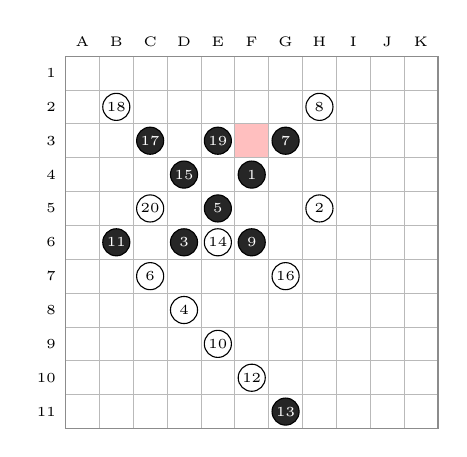
\begin{tikzpicture}[x=0.43cm, y=0.43cm]
\fill[red!25] (5,-2) rectangle (6,-3);
\draw[gray!55, line width=.3pt, step=1] (0,0) grid (11,-11);
\draw[gray!90] (0,0) rectangle (11,-11);
\node[font=\tiny, anchor=south] at (0.5,0) {A};
\node[font=\tiny, anchor=south] at (1.5,0) {B};
\node[font=\tiny, anchor=south] at (2.5,0) {C};
\node[font=\tiny, anchor=south] at (3.5,0) {D};
\node[font=\tiny, anchor=south] at (4.5,0) {E};
\node[font=\tiny, anchor=south] at (5.5,0) {F};
\node[font=\tiny, anchor=south] at (6.5,0) {G};
\node[font=\tiny, anchor=south] at (7.5,0) {H};
\node[font=\tiny, anchor=south] at (8.5,0) {I};
\node[font=\tiny, anchor=south] at (9.5,0) {J};
\node[font=\tiny, anchor=south] at (10.5,0) {K};
\node[font=\tiny, anchor=east] at (0,-0.5) {1};
\node[font=\tiny, anchor=east] at (0,-1.5) {2};
\node[font=\tiny, anchor=east] at (0,-2.5) {3};
\node[font=\tiny, anchor=east] at (0,-3.5) {4};
\node[font=\tiny, anchor=east] at (0,-4.5) {5};
\node[font=\tiny, anchor=east] at (0,-5.5) {6};
\node[font=\tiny, anchor=east] at (0,-6.5) {7};
\node[font=\tiny, anchor=east] at (0,-7.5) {8};
\node[font=\tiny, anchor=east] at (0,-8.5) {9};
\node[font=\tiny, anchor=east] at (0,-9.5) {10};
\node[font=\tiny, anchor=east] at (0,-10.5) {11};
\draw[fill=white, line width=.4pt] (1.5,-1.5) circle (.40);
\node[font=\tiny, text=black, inner sep=0pt] at (1.5,-1.5) {18};
\draw[fill=white, line width=.4pt] (7.5,-1.5) circle (.40);
\node[font=\tiny, text=black, inner sep=0pt] at (7.5,-1.5) {8};
\draw[fill=black!85, line width=.4pt] (2.5,-2.5) circle (.40);
\node[font=\tiny, text=white, inner sep=0pt] at (2.5,-2.5) {17};
\draw[fill=black!85, line width=.4pt] (4.5,-2.5) circle (.40);
\node[font=\tiny, text=white, inner sep=0pt] at (4.5,-2.5) {19};
\draw[fill=black!85, line width=.4pt] (6.5,-2.5) circle (.40);
\node[font=\tiny, text=white, inner sep=0pt] at (6.5,-2.5) {7};
\draw[fill=black!85, line width=.4pt] (3.5,-3.5) circle (.40);
\node[font=\tiny, text=white, inner sep=0pt] at (3.5,-3.5) {15};
\draw[fill=black!85, line width=.4pt] (5.5,-3.5) circle (.40);
\node[font=\tiny, text=white, inner sep=0pt] at (5.5,-3.5) {1};
\draw[fill=white, line width=.4pt] (2.5,-4.5) circle (.40);
\node[font=\tiny, text=black, inner sep=0pt] at (2.5,-4.5) {20};
\draw[fill=black!85, line width=.4pt] (4.5,-4.5) circle (.40);
\node[font=\tiny, text=white, inner sep=0pt] at (4.5,-4.5) {5};
\draw[fill=white, line width=.4pt] (7.5,-4.5) circle (.40);
\node[font=\tiny, text=black, inner sep=0pt] at (7.5,-4.5) {2};
\draw[fill=black!85, line width=.4pt] (1.5,-5.5) circle (.40);
\node[font=\tiny, text=white, inner sep=0pt] at (1.5,-5.5) {11};
\draw[fill=black!85, line width=.4pt] (3.5,-5.5) circle (.40);
\node[font=\tiny, text=white, inner sep=0pt] at (3.5,-5.5) {3};
\draw[fill=white, line width=.4pt] (4.5,-5.5) circle (.40);
\node[font=\tiny, text=black, inner sep=0pt] at (4.5,-5.5) {14};
\draw[fill=black!85, line width=.4pt] (5.5,-5.5) circle (.40);
\node[font=\tiny, text=white, inner sep=0pt] at (5.5,-5.5) {9};
\draw[fill=white, line width=.4pt] (2.5,-6.5) circle (.40);
\node[font=\tiny, text=black, inner sep=0pt] at (2.5,-6.5) {6};
\draw[fill=white, line width=.4pt] (6.5,-6.5) circle (.40);
\node[font=\tiny, text=black, inner sep=0pt] at (6.5,-6.5) {16};
\draw[fill=white, line width=.4pt] (3.5,-7.5) circle (.40);
\node[font=\tiny, text=black, inner sep=0pt] at (3.5,-7.5) {4};
\draw[fill=white, line width=.4pt] (4.5,-8.5) circle (.40);
\node[font=\tiny, text=black, inner sep=0pt] at (4.5,-8.5) {10};
\draw[fill=white, line width=.4pt] (5.5,-9.5) circle (.40);
\node[font=\tiny, text=black, inner sep=0pt] at (5.5,-9.5) {12};
\draw[fill=black!85, line width=.4pt] (6.5,-10.5) circle (.40);
\node[font=\tiny, text=white, inner sep=0pt] at (6.5,-10.5) {13};
\end{tikzpicture}
    \caption{Trước nước 21 (X đi; ô đỏ là nước đã chọn)}
  \end{subfigure}\hfill
  \begin{subfigure}[t]{.48\linewidth}
    \centering
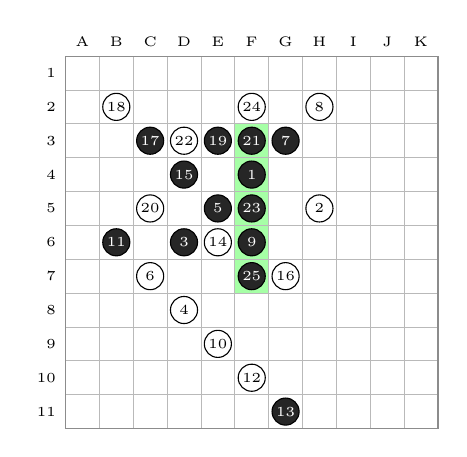
\begin{tikzpicture}[x=0.43cm, y=0.43cm]
\fill[green!35] (5,-6) rectangle (6,-7);
\fill[green!35] (5,-5) rectangle (6,-6);
\fill[green!35] (5,-4) rectangle (6,-5);
\fill[green!35] (5,-3) rectangle (6,-4);
\fill[green!35] (5,-2) rectangle (6,-3);
\draw[gray!55, line width=.3pt, step=1] (0,0) grid (11,-11);
\draw[gray!90] (0,0) rectangle (11,-11);
\node[font=\tiny, anchor=south] at (0.5,0) {A};
\node[font=\tiny, anchor=south] at (1.5,0) {B};
\node[font=\tiny, anchor=south] at (2.5,0) {C};
\node[font=\tiny, anchor=south] at (3.5,0) {D};
\node[font=\tiny, anchor=south] at (4.5,0) {E};
\node[font=\tiny, anchor=south] at (5.5,0) {F};
\node[font=\tiny, anchor=south] at (6.5,0) {G};
\node[font=\tiny, anchor=south] at (7.5,0) {H};
\node[font=\tiny, anchor=south] at (8.5,0) {I};
\node[font=\tiny, anchor=south] at (9.5,0) {J};
\node[font=\tiny, anchor=south] at (10.5,0) {K};
\node[font=\tiny, anchor=east] at (0,-0.5) {1};
\node[font=\tiny, anchor=east] at (0,-1.5) {2};
\node[font=\tiny, anchor=east] at (0,-2.5) {3};
\node[font=\tiny, anchor=east] at (0,-3.5) {4};
\node[font=\tiny, anchor=east] at (0,-4.5) {5};
\node[font=\tiny, anchor=east] at (0,-5.5) {6};
\node[font=\tiny, anchor=east] at (0,-6.5) {7};
\node[font=\tiny, anchor=east] at (0,-7.5) {8};
\node[font=\tiny, anchor=east] at (0,-8.5) {9};
\node[font=\tiny, anchor=east] at (0,-9.5) {10};
\node[font=\tiny, anchor=east] at (0,-10.5) {11};
\draw[fill=white, line width=.4pt] (1.5,-1.5) circle (.40);
\node[font=\tiny, text=black, inner sep=0pt] at (1.5,-1.5) {18};
\draw[fill=white, line width=.4pt] (5.5,-1.5) circle (.40);
\node[font=\tiny, text=black, inner sep=0pt] at (5.5,-1.5) {24};
\draw[fill=white, line width=.4pt] (7.5,-1.5) circle (.40);
\node[font=\tiny, text=black, inner sep=0pt] at (7.5,-1.5) {8};
\draw[fill=black!85, line width=.4pt] (2.5,-2.5) circle (.40);
\node[font=\tiny, text=white, inner sep=0pt] at (2.5,-2.5) {17};
\draw[fill=white, line width=.4pt] (3.5,-2.5) circle (.40);
\node[font=\tiny, text=black, inner sep=0pt] at (3.5,-2.5) {22};
\draw[fill=black!85, line width=.4pt] (4.5,-2.5) circle (.40);
\node[font=\tiny, text=white, inner sep=0pt] at (4.5,-2.5) {19};
\draw[fill=black!85, line width=.4pt] (5.5,-2.5) circle (.40);
\node[font=\tiny, text=white, inner sep=0pt] at (5.5,-2.5) {21};
\draw[fill=black!85, line width=.4pt] (6.5,-2.5) circle (.40);
\node[font=\tiny, text=white, inner sep=0pt] at (6.5,-2.5) {7};
\draw[fill=black!85, line width=.4pt] (3.5,-3.5) circle (.40);
\node[font=\tiny, text=white, inner sep=0pt] at (3.5,-3.5) {15};
\draw[fill=black!85, line width=.4pt] (5.5,-3.5) circle (.40);
\node[font=\tiny, text=white, inner sep=0pt] at (5.5,-3.5) {1};
\draw[fill=white, line width=.4pt] (2.5,-4.5) circle (.40);
\node[font=\tiny, text=black, inner sep=0pt] at (2.5,-4.5) {20};
\draw[fill=black!85, line width=.4pt] (4.5,-4.5) circle (.40);
\node[font=\tiny, text=white, inner sep=0pt] at (4.5,-4.5) {5};
\draw[fill=black!85, line width=.4pt] (5.5,-4.5) circle (.40);
\node[font=\tiny, text=white, inner sep=0pt] at (5.5,-4.5) {23};
\draw[fill=white, line width=.4pt] (7.5,-4.5) circle (.40);
\node[font=\tiny, text=black, inner sep=0pt] at (7.5,-4.5) {2};
\draw[fill=black!85, line width=.4pt] (1.5,-5.5) circle (.40);
\node[font=\tiny, text=white, inner sep=0pt] at (1.5,-5.5) {11};
\draw[fill=black!85, line width=.4pt] (3.5,-5.5) circle (.40);
\node[font=\tiny, text=white, inner sep=0pt] at (3.5,-5.5) {3};
\draw[fill=white, line width=.4pt] (4.5,-5.5) circle (.40);
\node[font=\tiny, text=black, inner sep=0pt] at (4.5,-5.5) {14};
\draw[fill=black!85, line width=.4pt] (5.5,-5.5) circle (.40);
\node[font=\tiny, text=white, inner sep=0pt] at (5.5,-5.5) {9};
\draw[fill=white, line width=.4pt] (2.5,-6.5) circle (.40);
\node[font=\tiny, text=black, inner sep=0pt] at (2.5,-6.5) {6};
\draw[fill=black!85, line width=.4pt] (5.5,-6.5) circle (.40);
\node[font=\tiny, text=white, inner sep=0pt] at (5.5,-6.5) {25};
\draw[fill=white, line width=.4pt] (6.5,-6.5) circle (.40);
\node[font=\tiny, text=black, inner sep=0pt] at (6.5,-6.5) {16};
\draw[fill=white, line width=.4pt] (3.5,-7.5) circle (.40);
\node[font=\tiny, text=black, inner sep=0pt] at (3.5,-7.5) {4};
\draw[fill=white, line width=.4pt] (4.5,-8.5) circle (.40);
\node[font=\tiny, text=black, inner sep=0pt] at (4.5,-8.5) {10};
\draw[fill=white, line width=.4pt] (5.5,-9.5) circle (.40);
\node[font=\tiny, text=black, inner sep=0pt] at (5.5,-9.5) {12};
\draw[fill=black!85, line width=.4pt] (6.5,-10.5) circle (.40);
\node[font=\tiny, text=white, inner sep=0pt] at (6.5,-10.5) {13};
\end{tikzpicture}
    \caption{Thế cuối (ô xanh: dãy thắng)}
  \end{subfigure}
  \caption{Ván 1202 (L2 cầm X, L8 cầm O).}
  \label{fig:cs-van-13}
\end{figure}
{\footnotesize\linespread{1}\selectfont
\noindent\begin{tabularx}{\linewidth}{*{6}{X}}
\toprule
1.~X F4$^\ast$ & 6.~O C7 & 11.~X B6 & 16.~O G7 & 21.~X F3 &  \\
2.~O H5$^\ast$ & 7.~X G3 & 12.~O F10 & 17.~X C3 & 22.~O D3 &  \\
3.~X D6$^\ast$ & 8.~O H2 & 13.~X G11 & 18.~O B2 & 23.~X F5 &  \\
4.~O D8$^\ast$ & 9.~X F6 & 14.~O E6 & 19.~X E3 & 24.~O F2 &  \\
5.~X E5 & 10.~O E9 & 15.~X D4 & 20.~O C5 & 25.~X F7 &  \\
\bottomrule
\end{tabularx}\par}
\paragraph{Diễn biến chiến thuật.}
\begin{itemize}\small
\setlength{\itemsep}{0pt}
  \item Nước 8 (O=L8, H2): chặn ô thắng H2.
  \item Nước 13 (X=L2, G11): chặn ô thắng G11.
  \item Nước 18 (O=L8, B2): chặn ô thắng B2.
  \item Nước 20 (O=L8, C5): không còn nước nào ngăn được VCF của đối thủ.
  \item Nước 21 (X=L2, F3): đang có VCF 3 nước và đi đúng một đường (D3--F3--D5--D2--D7 là đường ngắn nhất).
  \item Nước 22 (O=L8, D3): chặn ô thắng D3.
  \item Nước 23 (X=L2, F5): đang có VCF 2 nước và đi đúng một đường (F5--F2--F7 là đường ngắn nhất).
  \item Nước 24 (O=L8, F2): đối thủ đang có các ô thắng F2, F7, không đỡ hết được.
  \item Nước 25 (X=L2, F7): thắng ngay.
\end{itemize}
Thời gian trung vị mỗi nước: X 2,4 ms, O 91,3 ms.
\clearpage

\subsection{L3 -- L4: ván 1332}
\label{sec:cs-van-14}
X: \texttt{L3-AlphaBeta}; O: \texttt{L4-MCTS}; khai cuộc 16 (3 nước, đánh dấu $\ast$); 11 nước; kết quả: X (L3) thắng. Cả cặp: L3 thắng 100, hoà 0, thua 0 trên 100 ván; trung vị 11 nước.
\begin{figure}[H]
  \centering
  \begin{subfigure}[t]{.48\linewidth}
    \centering
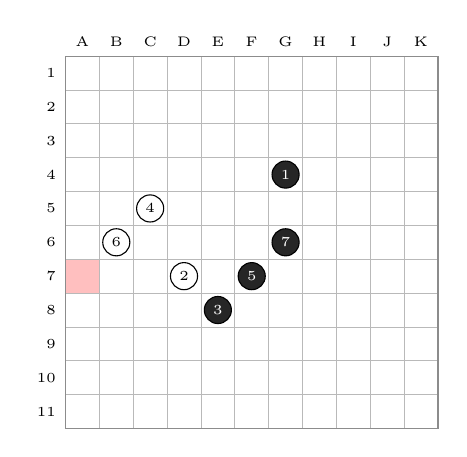
\begin{tikzpicture}[x=0.43cm, y=0.43cm]
\fill[red!25] (0,-6) rectangle (1,-7);
\draw[gray!55, line width=.3pt, step=1] (0,0) grid (11,-11);
\draw[gray!90] (0,0) rectangle (11,-11);
\node[font=\tiny, anchor=south] at (0.5,0) {A};
\node[font=\tiny, anchor=south] at (1.5,0) {B};
\node[font=\tiny, anchor=south] at (2.5,0) {C};
\node[font=\tiny, anchor=south] at (3.5,0) {D};
\node[font=\tiny, anchor=south] at (4.5,0) {E};
\node[font=\tiny, anchor=south] at (5.5,0) {F};
\node[font=\tiny, anchor=south] at (6.5,0) {G};
\node[font=\tiny, anchor=south] at (7.5,0) {H};
\node[font=\tiny, anchor=south] at (8.5,0) {I};
\node[font=\tiny, anchor=south] at (9.5,0) {J};
\node[font=\tiny, anchor=south] at (10.5,0) {K};
\node[font=\tiny, anchor=east] at (0,-0.5) {1};
\node[font=\tiny, anchor=east] at (0,-1.5) {2};
\node[font=\tiny, anchor=east] at (0,-2.5) {3};
\node[font=\tiny, anchor=east] at (0,-3.5) {4};
\node[font=\tiny, anchor=east] at (0,-4.5) {5};
\node[font=\tiny, anchor=east] at (0,-5.5) {6};
\node[font=\tiny, anchor=east] at (0,-6.5) {7};
\node[font=\tiny, anchor=east] at (0,-7.5) {8};
\node[font=\tiny, anchor=east] at (0,-8.5) {9};
\node[font=\tiny, anchor=east] at (0,-9.5) {10};
\node[font=\tiny, anchor=east] at (0,-10.5) {11};
\draw[fill=black!85, line width=.4pt] (6.5,-3.5) circle (.40);
\node[font=\tiny, text=white, inner sep=0pt] at (6.5,-3.5) {1};
\draw[fill=white, line width=.4pt] (2.5,-4.5) circle (.40);
\node[font=\tiny, text=black, inner sep=0pt] at (2.5,-4.5) {4};
\draw[fill=white, line width=.4pt] (1.5,-5.5) circle (.40);
\node[font=\tiny, text=black, inner sep=0pt] at (1.5,-5.5) {6};
\draw[fill=black!85, line width=.4pt] (6.5,-5.5) circle (.40);
\node[font=\tiny, text=white, inner sep=0pt] at (6.5,-5.5) {7};
\draw[fill=white, line width=.4pt] (3.5,-6.5) circle (.40);
\node[font=\tiny, text=black, inner sep=0pt] at (3.5,-6.5) {2};
\draw[fill=black!85, line width=.4pt] (5.5,-6.5) circle (.40);
\node[font=\tiny, text=white, inner sep=0pt] at (5.5,-6.5) {5};
\draw[fill=black!85, line width=.4pt] (4.5,-7.5) circle (.40);
\node[font=\tiny, text=white, inner sep=0pt] at (4.5,-7.5) {3};
\end{tikzpicture}
    \caption{Trước nước 8 (O đi; ô đỏ là nước đã chọn)}
  \end{subfigure}\hfill
  \begin{subfigure}[t]{.48\linewidth}
    \centering
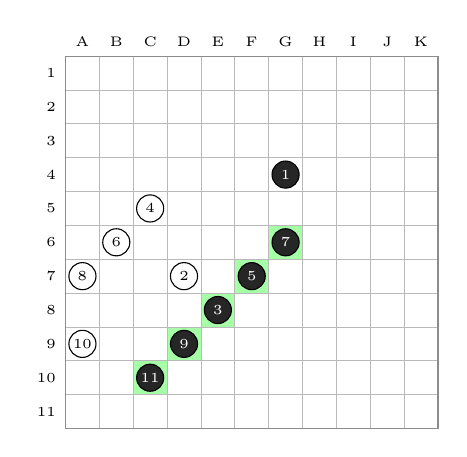
\begin{tikzpicture}[x=0.43cm, y=0.43cm]
\fill[green!35] (2,-9) rectangle (3,-10);
\fill[green!35] (3,-8) rectangle (4,-9);
\fill[green!35] (4,-7) rectangle (5,-8);
\fill[green!35] (5,-6) rectangle (6,-7);
\fill[green!35] (6,-5) rectangle (7,-6);
\draw[gray!55, line width=.3pt, step=1] (0,0) grid (11,-11);
\draw[gray!90] (0,0) rectangle (11,-11);
\node[font=\tiny, anchor=south] at (0.5,0) {A};
\node[font=\tiny, anchor=south] at (1.5,0) {B};
\node[font=\tiny, anchor=south] at (2.5,0) {C};
\node[font=\tiny, anchor=south] at (3.5,0) {D};
\node[font=\tiny, anchor=south] at (4.5,0) {E};
\node[font=\tiny, anchor=south] at (5.5,0) {F};
\node[font=\tiny, anchor=south] at (6.5,0) {G};
\node[font=\tiny, anchor=south] at (7.5,0) {H};
\node[font=\tiny, anchor=south] at (8.5,0) {I};
\node[font=\tiny, anchor=south] at (9.5,0) {J};
\node[font=\tiny, anchor=south] at (10.5,0) {K};
\node[font=\tiny, anchor=east] at (0,-0.5) {1};
\node[font=\tiny, anchor=east] at (0,-1.5) {2};
\node[font=\tiny, anchor=east] at (0,-2.5) {3};
\node[font=\tiny, anchor=east] at (0,-3.5) {4};
\node[font=\tiny, anchor=east] at (0,-4.5) {5};
\node[font=\tiny, anchor=east] at (0,-5.5) {6};
\node[font=\tiny, anchor=east] at (0,-6.5) {7};
\node[font=\tiny, anchor=east] at (0,-7.5) {8};
\node[font=\tiny, anchor=east] at (0,-8.5) {9};
\node[font=\tiny, anchor=east] at (0,-9.5) {10};
\node[font=\tiny, anchor=east] at (0,-10.5) {11};
\draw[fill=black!85, line width=.4pt] (6.5,-3.5) circle (.40);
\node[font=\tiny, text=white, inner sep=0pt] at (6.5,-3.5) {1};
\draw[fill=white, line width=.4pt] (2.5,-4.5) circle (.40);
\node[font=\tiny, text=black, inner sep=0pt] at (2.5,-4.5) {4};
\draw[fill=white, line width=.4pt] (1.5,-5.5) circle (.40);
\node[font=\tiny, text=black, inner sep=0pt] at (1.5,-5.5) {6};
\draw[fill=black!85, line width=.4pt] (6.5,-5.5) circle (.40);
\node[font=\tiny, text=white, inner sep=0pt] at (6.5,-5.5) {7};
\draw[fill=white, line width=.4pt] (0.5,-6.5) circle (.40);
\node[font=\tiny, text=black, inner sep=0pt] at (0.5,-6.5) {8};
\draw[fill=white, line width=.4pt] (3.5,-6.5) circle (.40);
\node[font=\tiny, text=black, inner sep=0pt] at (3.5,-6.5) {2};
\draw[fill=black!85, line width=.4pt] (5.5,-6.5) circle (.40);
\node[font=\tiny, text=white, inner sep=0pt] at (5.5,-6.5) {5};
\draw[fill=black!85, line width=.4pt] (4.5,-7.5) circle (.40);
\node[font=\tiny, text=white, inner sep=0pt] at (4.5,-7.5) {3};
\draw[fill=white, line width=.4pt] (0.5,-8.5) circle (.40);
\node[font=\tiny, text=black, inner sep=0pt] at (0.5,-8.5) {10};
\draw[fill=black!85, line width=.4pt] (3.5,-8.5) circle (.40);
\node[font=\tiny, text=white, inner sep=0pt] at (3.5,-8.5) {9};
\draw[fill=black!85, line width=.4pt] (2.5,-9.5) circle (.40);
\node[font=\tiny, text=white, inner sep=0pt] at (2.5,-9.5) {11};
\end{tikzpicture}
    \caption{Thế cuối (ô xanh: dãy thắng)}
  \end{subfigure}
  \caption{Ván 1332 (L3 cầm X, L4 cầm O).}
  \label{fig:cs-van-14}
\end{figure}
{\footnotesize\linespread{1}\selectfont
\noindent\begin{tabularx}{\linewidth}{*{6}{X}}
\toprule
1.~X G4$^\ast$ & 3.~X E8$^\ast$ & 5.~X F7 & 7.~X G6 & 9.~X D9 & 11.~X C10 \\
2.~O D7$^\ast$ & 4.~O C5 & 6.~O B6 & 8.~O A7 & 10.~O A9 &  \\
\bottomrule
\end{tabularx}\par}
\paragraph{Diễn biến chiến thuật.}
\begin{itemize}\small
\setlength{\itemsep}{0pt}
  \item Nước 8 (O=L4, A7): để đối thủ có VCF: H5--I4--D9.
  \item Nước 9 (X=L3, D9): đang có VCF 2 nước và đi đúng một đường (H5--I4--D9 là đường ngắn nhất).
  \item Nước 10 (O=L4, A9): đối thủ đang có các ô thắng H5, C10, không đỡ hết được.
  \item Nước 11 (X=L3, C10): thắng ngay.
\end{itemize}
Thời gian trung vị mỗi nước: X 11,0 ms, O 63,4 ms.
\clearpage

\subsection{L3 -- L5: ván 1482}
\label{sec:cs-van-15}
X: \texttt{L3-AlphaBeta}; O: \texttt{L5-PolicySL}; khai cuộc 41 (2 nước, đánh dấu $\ast$); 27 nước; kết quả: X (L3) thắng. Cả cặp: L3 thắng 63, hoà 3, thua 34 trên 100 ván; trung vị 28 nước.
\begin{figure}[H]
  \centering
  \begin{subfigure}[t]{.48\linewidth}
    \centering
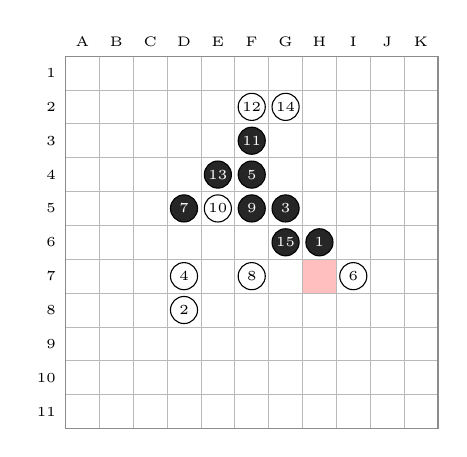
\begin{tikzpicture}[x=0.43cm, y=0.43cm]
\fill[red!25] (7,-6) rectangle (8,-7);
\draw[gray!55, line width=.3pt, step=1] (0,0) grid (11,-11);
\draw[gray!90] (0,0) rectangle (11,-11);
\node[font=\tiny, anchor=south] at (0.5,0) {A};
\node[font=\tiny, anchor=south] at (1.5,0) {B};
\node[font=\tiny, anchor=south] at (2.5,0) {C};
\node[font=\tiny, anchor=south] at (3.5,0) {D};
\node[font=\tiny, anchor=south] at (4.5,0) {E};
\node[font=\tiny, anchor=south] at (5.5,0) {F};
\node[font=\tiny, anchor=south] at (6.5,0) {G};
\node[font=\tiny, anchor=south] at (7.5,0) {H};
\node[font=\tiny, anchor=south] at (8.5,0) {I};
\node[font=\tiny, anchor=south] at (9.5,0) {J};
\node[font=\tiny, anchor=south] at (10.5,0) {K};
\node[font=\tiny, anchor=east] at (0,-0.5) {1};
\node[font=\tiny, anchor=east] at (0,-1.5) {2};
\node[font=\tiny, anchor=east] at (0,-2.5) {3};
\node[font=\tiny, anchor=east] at (0,-3.5) {4};
\node[font=\tiny, anchor=east] at (0,-4.5) {5};
\node[font=\tiny, anchor=east] at (0,-5.5) {6};
\node[font=\tiny, anchor=east] at (0,-6.5) {7};
\node[font=\tiny, anchor=east] at (0,-7.5) {8};
\node[font=\tiny, anchor=east] at (0,-8.5) {9};
\node[font=\tiny, anchor=east] at (0,-9.5) {10};
\node[font=\tiny, anchor=east] at (0,-10.5) {11};
\draw[fill=white, line width=.4pt] (5.5,-1.5) circle (.40);
\node[font=\tiny, text=black, inner sep=0pt] at (5.5,-1.5) {12};
\draw[fill=white, line width=.4pt] (6.5,-1.5) circle (.40);
\node[font=\tiny, text=black, inner sep=0pt] at (6.5,-1.5) {14};
\draw[fill=black!85, line width=.4pt] (5.5,-2.5) circle (.40);
\node[font=\tiny, text=white, inner sep=0pt] at (5.5,-2.5) {11};
\draw[fill=black!85, line width=.4pt] (4.5,-3.5) circle (.40);
\node[font=\tiny, text=white, inner sep=0pt] at (4.5,-3.5) {13};
\draw[fill=black!85, line width=.4pt] (5.5,-3.5) circle (.40);
\node[font=\tiny, text=white, inner sep=0pt] at (5.5,-3.5) {5};
\draw[fill=black!85, line width=.4pt] (3.5,-4.5) circle (.40);
\node[font=\tiny, text=white, inner sep=0pt] at (3.5,-4.5) {7};
\draw[fill=white, line width=.4pt] (4.5,-4.5) circle (.40);
\node[font=\tiny, text=black, inner sep=0pt] at (4.5,-4.5) {10};
\draw[fill=black!85, line width=.4pt] (5.5,-4.5) circle (.40);
\node[font=\tiny, text=white, inner sep=0pt] at (5.5,-4.5) {9};
\draw[fill=black!85, line width=.4pt] (6.5,-4.5) circle (.40);
\node[font=\tiny, text=white, inner sep=0pt] at (6.5,-4.5) {3};
\draw[fill=black!85, line width=.4pt] (6.5,-5.5) circle (.40);
\node[font=\tiny, text=white, inner sep=0pt] at (6.5,-5.5) {15};
\draw[fill=black!85, line width=.4pt] (7.5,-5.5) circle (.40);
\node[font=\tiny, text=white, inner sep=0pt] at (7.5,-5.5) {1};
\draw[fill=white, line width=.4pt] (3.5,-6.5) circle (.40);
\node[font=\tiny, text=black, inner sep=0pt] at (3.5,-6.5) {4};
\draw[fill=white, line width=.4pt] (5.5,-6.5) circle (.40);
\node[font=\tiny, text=black, inner sep=0pt] at (5.5,-6.5) {8};
\draw[fill=white, line width=.4pt] (8.5,-6.5) circle (.40);
\node[font=\tiny, text=black, inner sep=0pt] at (8.5,-6.5) {6};
\draw[fill=white, line width=.4pt] (3.5,-7.5) circle (.40);
\node[font=\tiny, text=black, inner sep=0pt] at (3.5,-7.5) {2};
\end{tikzpicture}
    \caption{Trước nước 16 (O đi; ô đỏ là nước đã chọn)}
  \end{subfigure}\hfill
  \begin{subfigure}[t]{.48\linewidth}
    \centering
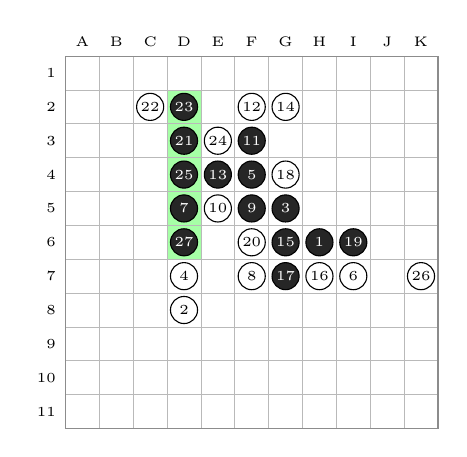
\begin{tikzpicture}[x=0.43cm, y=0.43cm]
\fill[green!35] (3,-5) rectangle (4,-6);
\fill[green!35] (3,-4) rectangle (4,-5);
\fill[green!35] (3,-3) rectangle (4,-4);
\fill[green!35] (3,-2) rectangle (4,-3);
\fill[green!35] (3,-1) rectangle (4,-2);
\draw[gray!55, line width=.3pt, step=1] (0,0) grid (11,-11);
\draw[gray!90] (0,0) rectangle (11,-11);
\node[font=\tiny, anchor=south] at (0.5,0) {A};
\node[font=\tiny, anchor=south] at (1.5,0) {B};
\node[font=\tiny, anchor=south] at (2.5,0) {C};
\node[font=\tiny, anchor=south] at (3.5,0) {D};
\node[font=\tiny, anchor=south] at (4.5,0) {E};
\node[font=\tiny, anchor=south] at (5.5,0) {F};
\node[font=\tiny, anchor=south] at (6.5,0) {G};
\node[font=\tiny, anchor=south] at (7.5,0) {H};
\node[font=\tiny, anchor=south] at (8.5,0) {I};
\node[font=\tiny, anchor=south] at (9.5,0) {J};
\node[font=\tiny, anchor=south] at (10.5,0) {K};
\node[font=\tiny, anchor=east] at (0,-0.5) {1};
\node[font=\tiny, anchor=east] at (0,-1.5) {2};
\node[font=\tiny, anchor=east] at (0,-2.5) {3};
\node[font=\tiny, anchor=east] at (0,-3.5) {4};
\node[font=\tiny, anchor=east] at (0,-4.5) {5};
\node[font=\tiny, anchor=east] at (0,-5.5) {6};
\node[font=\tiny, anchor=east] at (0,-6.5) {7};
\node[font=\tiny, anchor=east] at (0,-7.5) {8};
\node[font=\tiny, anchor=east] at (0,-8.5) {9};
\node[font=\tiny, anchor=east] at (0,-9.5) {10};
\node[font=\tiny, anchor=east] at (0,-10.5) {11};
\draw[fill=white, line width=.4pt] (2.5,-1.5) circle (.40);
\node[font=\tiny, text=black, inner sep=0pt] at (2.5,-1.5) {22};
\draw[fill=black!85, line width=.4pt] (3.5,-1.5) circle (.40);
\node[font=\tiny, text=white, inner sep=0pt] at (3.5,-1.5) {23};
\draw[fill=white, line width=.4pt] (5.5,-1.5) circle (.40);
\node[font=\tiny, text=black, inner sep=0pt] at (5.5,-1.5) {12};
\draw[fill=white, line width=.4pt] (6.5,-1.5) circle (.40);
\node[font=\tiny, text=black, inner sep=0pt] at (6.5,-1.5) {14};
\draw[fill=black!85, line width=.4pt] (3.5,-2.5) circle (.40);
\node[font=\tiny, text=white, inner sep=0pt] at (3.5,-2.5) {21};
\draw[fill=white, line width=.4pt] (4.5,-2.5) circle (.40);
\node[font=\tiny, text=black, inner sep=0pt] at (4.5,-2.5) {24};
\draw[fill=black!85, line width=.4pt] (5.5,-2.5) circle (.40);
\node[font=\tiny, text=white, inner sep=0pt] at (5.5,-2.5) {11};
\draw[fill=black!85, line width=.4pt] (3.5,-3.5) circle (.40);
\node[font=\tiny, text=white, inner sep=0pt] at (3.5,-3.5) {25};
\draw[fill=black!85, line width=.4pt] (4.5,-3.5) circle (.40);
\node[font=\tiny, text=white, inner sep=0pt] at (4.5,-3.5) {13};
\draw[fill=black!85, line width=.4pt] (5.5,-3.5) circle (.40);
\node[font=\tiny, text=white, inner sep=0pt] at (5.5,-3.5) {5};
\draw[fill=white, line width=.4pt] (6.5,-3.5) circle (.40);
\node[font=\tiny, text=black, inner sep=0pt] at (6.5,-3.5) {18};
\draw[fill=black!85, line width=.4pt] (3.5,-4.5) circle (.40);
\node[font=\tiny, text=white, inner sep=0pt] at (3.5,-4.5) {7};
\draw[fill=white, line width=.4pt] (4.5,-4.5) circle (.40);
\node[font=\tiny, text=black, inner sep=0pt] at (4.5,-4.5) {10};
\draw[fill=black!85, line width=.4pt] (5.5,-4.5) circle (.40);
\node[font=\tiny, text=white, inner sep=0pt] at (5.5,-4.5) {9};
\draw[fill=black!85, line width=.4pt] (6.5,-4.5) circle (.40);
\node[font=\tiny, text=white, inner sep=0pt] at (6.5,-4.5) {3};
\draw[fill=black!85, line width=.4pt] (3.5,-5.5) circle (.40);
\node[font=\tiny, text=white, inner sep=0pt] at (3.5,-5.5) {27};
\draw[fill=white, line width=.4pt] (5.5,-5.5) circle (.40);
\node[font=\tiny, text=black, inner sep=0pt] at (5.5,-5.5) {20};
\draw[fill=black!85, line width=.4pt] (6.5,-5.5) circle (.40);
\node[font=\tiny, text=white, inner sep=0pt] at (6.5,-5.5) {15};
\draw[fill=black!85, line width=.4pt] (7.5,-5.5) circle (.40);
\node[font=\tiny, text=white, inner sep=0pt] at (7.5,-5.5) {1};
\draw[fill=black!85, line width=.4pt] (8.5,-5.5) circle (.40);
\node[font=\tiny, text=white, inner sep=0pt] at (8.5,-5.5) {19};
\draw[fill=white, line width=.4pt] (3.5,-6.5) circle (.40);
\node[font=\tiny, text=black, inner sep=0pt] at (3.5,-6.5) {4};
\draw[fill=white, line width=.4pt] (5.5,-6.5) circle (.40);
\node[font=\tiny, text=black, inner sep=0pt] at (5.5,-6.5) {8};
\draw[fill=black!85, line width=.4pt] (6.5,-6.5) circle (.40);
\node[font=\tiny, text=white, inner sep=0pt] at (6.5,-6.5) {17};
\draw[fill=white, line width=.4pt] (7.5,-6.5) circle (.40);
\node[font=\tiny, text=black, inner sep=0pt] at (7.5,-6.5) {16};
\draw[fill=white, line width=.4pt] (8.5,-6.5) circle (.40);
\node[font=\tiny, text=black, inner sep=0pt] at (8.5,-6.5) {6};
\draw[fill=white, line width=.4pt] (10.5,-6.5) circle (.40);
\node[font=\tiny, text=black, inner sep=0pt] at (10.5,-6.5) {26};
\draw[fill=white, line width=.4pt] (3.5,-7.5) circle (.40);
\node[font=\tiny, text=black, inner sep=0pt] at (3.5,-7.5) {2};
\end{tikzpicture}
    \caption{Thế cuối (ô xanh: dãy thắng)}
  \end{subfigure}
  \caption{Ván 1482 (L3 cầm X, L5 cầm O).}
  \label{fig:cs-van-15}
\end{figure}
{\footnotesize\linespread{1}\selectfont
\noindent\begin{tabularx}{\linewidth}{*{6}{X}}
\toprule
1.~X H6$^\ast$ & 6.~O I7 & 11.~X F3 & 16.~O H7 & 21.~X D3 & 26.~O K7 \\
2.~O D8$^\ast$ & 7.~X D5 & 12.~O F2 & 17.~X G7 & 22.~O C2 & 27.~X D6 \\
3.~X G5 & 8.~O F7 & 13.~X E4 & 18.~O G4 & 23.~X D2 &  \\
4.~O D7 & 9.~X F5 & 14.~O G2 & 19.~X I6 & 24.~O E3 &  \\
5.~X F4 & 10.~O E5 & 15.~X G6 & 20.~O F6 & 25.~X D4 &  \\
\bottomrule
\end{tabularx}\par}
\paragraph{Diễn biến chiến thuật.}
\begin{itemize}\small
\setlength{\itemsep}{0pt}
  \item Nước 16 (O=L5, H7): để đối thủ có VCF: D2--E3--D3--C2--D4--D1--D6.
  \item Nước 17 (X=L3, G7): bỏ lỡ VCF 4 nước: D2--E3--D3--C2--D4--D1--D6.
  \item Nước 18 (O=L5, G4): không còn nước nào ngăn được VCF của đối thủ.
  \item Nước 19 (X=L3, I6): bỏ lỡ VCF 4 nước: D2--E3--D3--C2--D4--D1--D6.
  \item Nước 20 (O=L5, F6): không còn nước nào ngăn được VCF của đối thủ.
  \item Nước 21 (X=L3, D3): đang có VCF 4 nước và đi đúng một đường (D2--E3--D3--C2--D4--D1--D6 là đường ngắn nhất).
  \item Nước 22 (O=L5, C2): chặn ô thắng C2.
  \item Nước 23 (X=L3, D2): đang có VCF 3 nước và đi đúng một đường (D2--E3--D4--D1--D6 là đường ngắn nhất).
  \item Nước 24 (O=L5, E3): chặn ô thắng E3.
  \item Nước 25 (X=L3, D4): đang có VCF 2 nước và đi đúng một đường (D4--D1--D6 là đường ngắn nhất).
  \item Nước 26 (O=L5, K7): đối thủ đang có các ô thắng D1, D6, không đỡ hết được.
  \item Nước 27 (X=L3, D6): thắng ngay.
\end{itemize}
Thời gian trung vị mỗi nước: X 26,3 ms, O 1,2 ms.
\clearpage

\subsection{L3 -- L6: ván 1592}
\label{sec:cs-van-16}
X: \texttt{L3-AlphaBeta}; O: \texttt{L6-PolicyRL}; khai cuộc 46 (3 nước, đánh dấu $\ast$); 25 nước; kết quả: X (L3) thắng. Cả cặp: L3 thắng 42, hoà 7, thua 51 trên 100 ván; trung vị 27 nước.
\begin{figure}[H]
  \centering
  \begin{subfigure}[t]{.48\linewidth}
    \centering
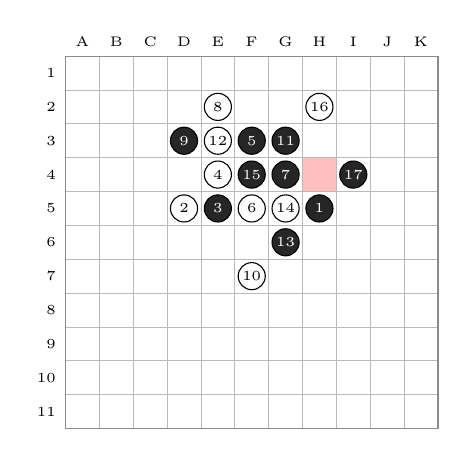
\begin{tikzpicture}[x=0.43cm, y=0.43cm]
\fill[red!25] (7,-3) rectangle (8,-4);
\draw[gray!55, line width=.3pt, step=1] (0,0) grid (11,-11);
\draw[gray!90] (0,0) rectangle (11,-11);
\node[font=\tiny, anchor=south] at (0.5,0) {A};
\node[font=\tiny, anchor=south] at (1.5,0) {B};
\node[font=\tiny, anchor=south] at (2.5,0) {C};
\node[font=\tiny, anchor=south] at (3.5,0) {D};
\node[font=\tiny, anchor=south] at (4.5,0) {E};
\node[font=\tiny, anchor=south] at (5.5,0) {F};
\node[font=\tiny, anchor=south] at (6.5,0) {G};
\node[font=\tiny, anchor=south] at (7.5,0) {H};
\node[font=\tiny, anchor=south] at (8.5,0) {I};
\node[font=\tiny, anchor=south] at (9.5,0) {J};
\node[font=\tiny, anchor=south] at (10.5,0) {K};
\node[font=\tiny, anchor=east] at (0,-0.5) {1};
\node[font=\tiny, anchor=east] at (0,-1.5) {2};
\node[font=\tiny, anchor=east] at (0,-2.5) {3};
\node[font=\tiny, anchor=east] at (0,-3.5) {4};
\node[font=\tiny, anchor=east] at (0,-4.5) {5};
\node[font=\tiny, anchor=east] at (0,-5.5) {6};
\node[font=\tiny, anchor=east] at (0,-6.5) {7};
\node[font=\tiny, anchor=east] at (0,-7.5) {8};
\node[font=\tiny, anchor=east] at (0,-8.5) {9};
\node[font=\tiny, anchor=east] at (0,-9.5) {10};
\node[font=\tiny, anchor=east] at (0,-10.5) {11};
\draw[fill=white, line width=.4pt] (4.5,-1.5) circle (.40);
\node[font=\tiny, text=black, inner sep=0pt] at (4.5,-1.5) {8};
\draw[fill=white, line width=.4pt] (7.5,-1.5) circle (.40);
\node[font=\tiny, text=black, inner sep=0pt] at (7.5,-1.5) {16};
\draw[fill=black!85, line width=.4pt] (3.5,-2.5) circle (.40);
\node[font=\tiny, text=white, inner sep=0pt] at (3.5,-2.5) {9};
\draw[fill=white, line width=.4pt] (4.5,-2.5) circle (.40);
\node[font=\tiny, text=black, inner sep=0pt] at (4.5,-2.5) {12};
\draw[fill=black!85, line width=.4pt] (5.5,-2.5) circle (.40);
\node[font=\tiny, text=white, inner sep=0pt] at (5.5,-2.5) {5};
\draw[fill=black!85, line width=.4pt] (6.5,-2.5) circle (.40);
\node[font=\tiny, text=white, inner sep=0pt] at (6.5,-2.5) {11};
\draw[fill=white, line width=.4pt] (4.5,-3.5) circle (.40);
\node[font=\tiny, text=black, inner sep=0pt] at (4.5,-3.5) {4};
\draw[fill=black!85, line width=.4pt] (5.5,-3.5) circle (.40);
\node[font=\tiny, text=white, inner sep=0pt] at (5.5,-3.5) {15};
\draw[fill=black!85, line width=.4pt] (6.5,-3.5) circle (.40);
\node[font=\tiny, text=white, inner sep=0pt] at (6.5,-3.5) {7};
\draw[fill=black!85, line width=.4pt] (8.5,-3.5) circle (.40);
\node[font=\tiny, text=white, inner sep=0pt] at (8.5,-3.5) {17};
\draw[fill=white, line width=.4pt] (3.5,-4.5) circle (.40);
\node[font=\tiny, text=black, inner sep=0pt] at (3.5,-4.5) {2};
\draw[fill=black!85, line width=.4pt] (4.5,-4.5) circle (.40);
\node[font=\tiny, text=white, inner sep=0pt] at (4.5,-4.5) {3};
\draw[fill=white, line width=.4pt] (5.5,-4.5) circle (.40);
\node[font=\tiny, text=black, inner sep=0pt] at (5.5,-4.5) {6};
\draw[fill=white, line width=.4pt] (6.5,-4.5) circle (.40);
\node[font=\tiny, text=black, inner sep=0pt] at (6.5,-4.5) {14};
\draw[fill=black!85, line width=.4pt] (7.5,-4.5) circle (.40);
\node[font=\tiny, text=white, inner sep=0pt] at (7.5,-4.5) {1};
\draw[fill=black!85, line width=.4pt] (6.5,-5.5) circle (.40);
\node[font=\tiny, text=white, inner sep=0pt] at (6.5,-5.5) {13};
\draw[fill=white, line width=.4pt] (5.5,-6.5) circle (.40);
\node[font=\tiny, text=black, inner sep=0pt] at (5.5,-6.5) {10};
\end{tikzpicture}
    \caption{Trước nước 18 (O đi; ô đỏ là nước đã chọn)}
  \end{subfigure}\hfill
  \begin{subfigure}[t]{.48\linewidth}
    \centering
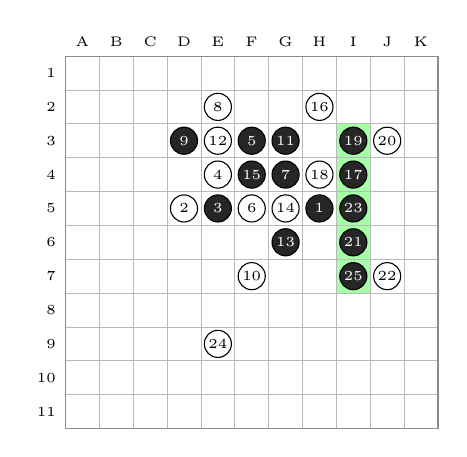
\begin{tikzpicture}[x=0.43cm, y=0.43cm]
\fill[green!35] (8,-6) rectangle (9,-7);
\fill[green!35] (8,-5) rectangle (9,-6);
\fill[green!35] (8,-4) rectangle (9,-5);
\fill[green!35] (8,-3) rectangle (9,-4);
\fill[green!35] (8,-2) rectangle (9,-3);
\draw[gray!55, line width=.3pt, step=1] (0,0) grid (11,-11);
\draw[gray!90] (0,0) rectangle (11,-11);
\node[font=\tiny, anchor=south] at (0.5,0) {A};
\node[font=\tiny, anchor=south] at (1.5,0) {B};
\node[font=\tiny, anchor=south] at (2.5,0) {C};
\node[font=\tiny, anchor=south] at (3.5,0) {D};
\node[font=\tiny, anchor=south] at (4.5,0) {E};
\node[font=\tiny, anchor=south] at (5.5,0) {F};
\node[font=\tiny, anchor=south] at (6.5,0) {G};
\node[font=\tiny, anchor=south] at (7.5,0) {H};
\node[font=\tiny, anchor=south] at (8.5,0) {I};
\node[font=\tiny, anchor=south] at (9.5,0) {J};
\node[font=\tiny, anchor=south] at (10.5,0) {K};
\node[font=\tiny, anchor=east] at (0,-0.5) {1};
\node[font=\tiny, anchor=east] at (0,-1.5) {2};
\node[font=\tiny, anchor=east] at (0,-2.5) {3};
\node[font=\tiny, anchor=east] at (0,-3.5) {4};
\node[font=\tiny, anchor=east] at (0,-4.5) {5};
\node[font=\tiny, anchor=east] at (0,-5.5) {6};
\node[font=\tiny, anchor=east] at (0,-6.5) {7};
\node[font=\tiny, anchor=east] at (0,-7.5) {8};
\node[font=\tiny, anchor=east] at (0,-8.5) {9};
\node[font=\tiny, anchor=east] at (0,-9.5) {10};
\node[font=\tiny, anchor=east] at (0,-10.5) {11};
\draw[fill=white, line width=.4pt] (4.5,-1.5) circle (.40);
\node[font=\tiny, text=black, inner sep=0pt] at (4.5,-1.5) {8};
\draw[fill=white, line width=.4pt] (7.5,-1.5) circle (.40);
\node[font=\tiny, text=black, inner sep=0pt] at (7.5,-1.5) {16};
\draw[fill=black!85, line width=.4pt] (3.5,-2.5) circle (.40);
\node[font=\tiny, text=white, inner sep=0pt] at (3.5,-2.5) {9};
\draw[fill=white, line width=.4pt] (4.5,-2.5) circle (.40);
\node[font=\tiny, text=black, inner sep=0pt] at (4.5,-2.5) {12};
\draw[fill=black!85, line width=.4pt] (5.5,-2.5) circle (.40);
\node[font=\tiny, text=white, inner sep=0pt] at (5.5,-2.5) {5};
\draw[fill=black!85, line width=.4pt] (6.5,-2.5) circle (.40);
\node[font=\tiny, text=white, inner sep=0pt] at (6.5,-2.5) {11};
\draw[fill=black!85, line width=.4pt] (8.5,-2.5) circle (.40);
\node[font=\tiny, text=white, inner sep=0pt] at (8.5,-2.5) {19};
\draw[fill=white, line width=.4pt] (9.5,-2.5) circle (.40);
\node[font=\tiny, text=black, inner sep=0pt] at (9.5,-2.5) {20};
\draw[fill=white, line width=.4pt] (4.5,-3.5) circle (.40);
\node[font=\tiny, text=black, inner sep=0pt] at (4.5,-3.5) {4};
\draw[fill=black!85, line width=.4pt] (5.5,-3.5) circle (.40);
\node[font=\tiny, text=white, inner sep=0pt] at (5.5,-3.5) {15};
\draw[fill=black!85, line width=.4pt] (6.5,-3.5) circle (.40);
\node[font=\tiny, text=white, inner sep=0pt] at (6.5,-3.5) {7};
\draw[fill=white, line width=.4pt] (7.5,-3.5) circle (.40);
\node[font=\tiny, text=black, inner sep=0pt] at (7.5,-3.5) {18};
\draw[fill=black!85, line width=.4pt] (8.5,-3.5) circle (.40);
\node[font=\tiny, text=white, inner sep=0pt] at (8.5,-3.5) {17};
\draw[fill=white, line width=.4pt] (3.5,-4.5) circle (.40);
\node[font=\tiny, text=black, inner sep=0pt] at (3.5,-4.5) {2};
\draw[fill=black!85, line width=.4pt] (4.5,-4.5) circle (.40);
\node[font=\tiny, text=white, inner sep=0pt] at (4.5,-4.5) {3};
\draw[fill=white, line width=.4pt] (5.5,-4.5) circle (.40);
\node[font=\tiny, text=black, inner sep=0pt] at (5.5,-4.5) {6};
\draw[fill=white, line width=.4pt] (6.5,-4.5) circle (.40);
\node[font=\tiny, text=black, inner sep=0pt] at (6.5,-4.5) {14};
\draw[fill=black!85, line width=.4pt] (7.5,-4.5) circle (.40);
\node[font=\tiny, text=white, inner sep=0pt] at (7.5,-4.5) {1};
\draw[fill=black!85, line width=.4pt] (8.5,-4.5) circle (.40);
\node[font=\tiny, text=white, inner sep=0pt] at (8.5,-4.5) {23};
\draw[fill=black!85, line width=.4pt] (6.5,-5.5) circle (.40);
\node[font=\tiny, text=white, inner sep=0pt] at (6.5,-5.5) {13};
\draw[fill=black!85, line width=.4pt] (8.5,-5.5) circle (.40);
\node[font=\tiny, text=white, inner sep=0pt] at (8.5,-5.5) {21};
\draw[fill=white, line width=.4pt] (5.5,-6.5) circle (.40);
\node[font=\tiny, text=black, inner sep=0pt] at (5.5,-6.5) {10};
\draw[fill=black!85, line width=.4pt] (8.5,-6.5) circle (.40);
\node[font=\tiny, text=white, inner sep=0pt] at (8.5,-6.5) {25};
\draw[fill=white, line width=.4pt] (9.5,-6.5) circle (.40);
\node[font=\tiny, text=black, inner sep=0pt] at (9.5,-6.5) {22};
\draw[fill=white, line width=.4pt] (4.5,-8.5) circle (.40);
\node[font=\tiny, text=black, inner sep=0pt] at (4.5,-8.5) {24};
\end{tikzpicture}
    \caption{Thế cuối (ô xanh: dãy thắng)}
  \end{subfigure}
  \caption{Ván 1592 (L3 cầm X, L6 cầm O).}
  \label{fig:cs-van-16}
\end{figure}
{\footnotesize\linespread{1}\selectfont
\noindent\begin{tabularx}{\linewidth}{*{6}{X}}
\toprule
1.~X H5$^\ast$ & 6.~O F5 & 11.~X G3 & 16.~O H2 & 21.~X I6 &  \\
2.~O D5$^\ast$ & 7.~X G4 & 12.~O E3 & 17.~X I4 & 22.~O J7 &  \\
3.~X E5$^\ast$ & 8.~O E2 & 13.~X G6 & 18.~O H4 & 23.~X I5 &  \\
4.~O E4 & 9.~X D3 & 14.~O G5 & 19.~X I3 & 24.~O E9 &  \\
5.~X F3 & 10.~O F7 & 15.~X F4 & 20.~O J3 & 25.~X I7 &  \\
\bottomrule
\end{tabularx}\par}
\paragraph{Diễn biến chiến thuật.}
\begin{itemize}\small
\setlength{\itemsep}{0pt}
  \item Nước 18 (O=L6, H4): để đối thủ có VCF: J3--K2--I3--H3--I6--J7--I5--I2--I7.
  \item Nước 19 (X=L3, I3): bỏ lỡ VCF 5 nước: J3--K2--I3--H3--I6--J7--I5--I2--I7.
  \item Nước 20 (O=L6, J3): không còn nước nào ngăn được VCF của đối thủ.
  \item Nước 21 (X=L3, I6): đang có VCF 3 nước và đi đúng một đường (I6--J7--I5--I2--I7 là đường ngắn nhất).
  \item Nước 22 (O=L6, J7): chặn ô thắng J7.
  \item Nước 23 (X=L3, I5): đang có VCF 2 nước và đi đúng một đường (I5--I2--I7 là đường ngắn nhất).
  \item Nước 24 (O=L6, E9): đối thủ đang có các ô thắng I2, I7, không đỡ hết được.
  \item Nước 25 (X=L3, I7): thắng ngay.
\end{itemize}
Thời gian trung vị mỗi nước: X 21,0 ms, O 1,1 ms.
\clearpage

\subsection{L3 -- L7: ván 1600}
\label{sec:cs-van-17}
X: \texttt{L3-AlphaBeta}; O: \texttt{L7-PUCT}; khai cuộc 0 (3 nước, đánh dấu $\ast$); 28 nước; kết quả: O (L7) thắng. Cả cặp: L3 thắng 16, hoà 6, thua 78 trên 100 ván; trung vị 29 nước.
\begin{figure}[H]
  \centering
  \begin{subfigure}[t]{.48\linewidth}
    \centering
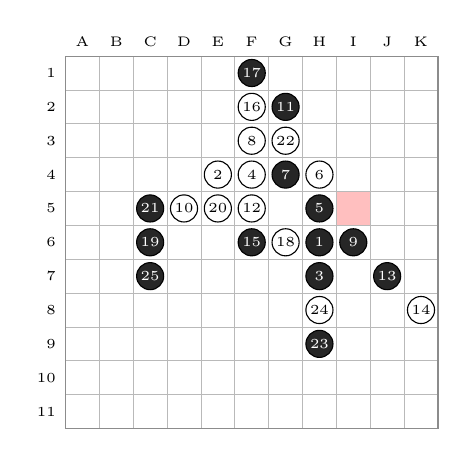
\begin{tikzpicture}[x=0.43cm, y=0.43cm]
\fill[red!25] (8,-4) rectangle (9,-5);
\draw[gray!55, line width=.3pt, step=1] (0,0) grid (11,-11);
\draw[gray!90] (0,0) rectangle (11,-11);
\node[font=\tiny, anchor=south] at (0.5,0) {A};
\node[font=\tiny, anchor=south] at (1.5,0) {B};
\node[font=\tiny, anchor=south] at (2.5,0) {C};
\node[font=\tiny, anchor=south] at (3.5,0) {D};
\node[font=\tiny, anchor=south] at (4.5,0) {E};
\node[font=\tiny, anchor=south] at (5.5,0) {F};
\node[font=\tiny, anchor=south] at (6.5,0) {G};
\node[font=\tiny, anchor=south] at (7.5,0) {H};
\node[font=\tiny, anchor=south] at (8.5,0) {I};
\node[font=\tiny, anchor=south] at (9.5,0) {J};
\node[font=\tiny, anchor=south] at (10.5,0) {K};
\node[font=\tiny, anchor=east] at (0,-0.5) {1};
\node[font=\tiny, anchor=east] at (0,-1.5) {2};
\node[font=\tiny, anchor=east] at (0,-2.5) {3};
\node[font=\tiny, anchor=east] at (0,-3.5) {4};
\node[font=\tiny, anchor=east] at (0,-4.5) {5};
\node[font=\tiny, anchor=east] at (0,-5.5) {6};
\node[font=\tiny, anchor=east] at (0,-6.5) {7};
\node[font=\tiny, anchor=east] at (0,-7.5) {8};
\node[font=\tiny, anchor=east] at (0,-8.5) {9};
\node[font=\tiny, anchor=east] at (0,-9.5) {10};
\node[font=\tiny, anchor=east] at (0,-10.5) {11};
\draw[fill=black!85, line width=.4pt] (5.5,-0.5) circle (.40);
\node[font=\tiny, text=white, inner sep=0pt] at (5.5,-0.5) {17};
\draw[fill=white, line width=.4pt] (5.5,-1.5) circle (.40);
\node[font=\tiny, text=black, inner sep=0pt] at (5.5,-1.5) {16};
\draw[fill=black!85, line width=.4pt] (6.5,-1.5) circle (.40);
\node[font=\tiny, text=white, inner sep=0pt] at (6.5,-1.5) {11};
\draw[fill=white, line width=.4pt] (5.5,-2.5) circle (.40);
\node[font=\tiny, text=black, inner sep=0pt] at (5.5,-2.5) {8};
\draw[fill=white, line width=.4pt] (6.5,-2.5) circle (.40);
\node[font=\tiny, text=black, inner sep=0pt] at (6.5,-2.5) {22};
\draw[fill=white, line width=.4pt] (4.5,-3.5) circle (.40);
\node[font=\tiny, text=black, inner sep=0pt] at (4.5,-3.5) {2};
\draw[fill=white, line width=.4pt] (5.5,-3.5) circle (.40);
\node[font=\tiny, text=black, inner sep=0pt] at (5.5,-3.5) {4};
\draw[fill=black!85, line width=.4pt] (6.5,-3.5) circle (.40);
\node[font=\tiny, text=white, inner sep=0pt] at (6.5,-3.5) {7};
\draw[fill=white, line width=.4pt] (7.5,-3.5) circle (.40);
\node[font=\tiny, text=black, inner sep=0pt] at (7.5,-3.5) {6};
\draw[fill=black!85, line width=.4pt] (2.5,-4.5) circle (.40);
\node[font=\tiny, text=white, inner sep=0pt] at (2.5,-4.5) {21};
\draw[fill=white, line width=.4pt] (3.5,-4.5) circle (.40);
\node[font=\tiny, text=black, inner sep=0pt] at (3.5,-4.5) {10};
\draw[fill=white, line width=.4pt] (4.5,-4.5) circle (.40);
\node[font=\tiny, text=black, inner sep=0pt] at (4.5,-4.5) {20};
\draw[fill=white, line width=.4pt] (5.5,-4.5) circle (.40);
\node[font=\tiny, text=black, inner sep=0pt] at (5.5,-4.5) {12};
\draw[fill=black!85, line width=.4pt] (7.5,-4.5) circle (.40);
\node[font=\tiny, text=white, inner sep=0pt] at (7.5,-4.5) {5};
\draw[fill=black!85, line width=.4pt] (2.5,-5.5) circle (.40);
\node[font=\tiny, text=white, inner sep=0pt] at (2.5,-5.5) {19};
\draw[fill=black!85, line width=.4pt] (5.5,-5.5) circle (.40);
\node[font=\tiny, text=white, inner sep=0pt] at (5.5,-5.5) {15};
\draw[fill=white, line width=.4pt] (6.5,-5.5) circle (.40);
\node[font=\tiny, text=black, inner sep=0pt] at (6.5,-5.5) {18};
\draw[fill=black!85, line width=.4pt] (7.5,-5.5) circle (.40);
\node[font=\tiny, text=white, inner sep=0pt] at (7.5,-5.5) {1};
\draw[fill=black!85, line width=.4pt] (8.5,-5.5) circle (.40);
\node[font=\tiny, text=white, inner sep=0pt] at (8.5,-5.5) {9};
\draw[fill=black!85, line width=.4pt] (2.5,-6.5) circle (.40);
\node[font=\tiny, text=white, inner sep=0pt] at (2.5,-6.5) {25};
\draw[fill=black!85, line width=.4pt] (7.5,-6.5) circle (.40);
\node[font=\tiny, text=white, inner sep=0pt] at (7.5,-6.5) {3};
\draw[fill=black!85, line width=.4pt] (9.5,-6.5) circle (.40);
\node[font=\tiny, text=white, inner sep=0pt] at (9.5,-6.5) {13};
\draw[fill=white, line width=.4pt] (7.5,-7.5) circle (.40);
\node[font=\tiny, text=black, inner sep=0pt] at (7.5,-7.5) {24};
\draw[fill=white, line width=.4pt] (10.5,-7.5) circle (.40);
\node[font=\tiny, text=black, inner sep=0pt] at (10.5,-7.5) {14};
\draw[fill=black!85, line width=.4pt] (7.5,-8.5) circle (.40);
\node[font=\tiny, text=white, inner sep=0pt] at (7.5,-8.5) {23};
\end{tikzpicture}
    \caption{Trước nước 26 (O đi; ô đỏ là nước đã chọn)}
  \end{subfigure}\hfill
  \begin{subfigure}[t]{.48\linewidth}
    \centering
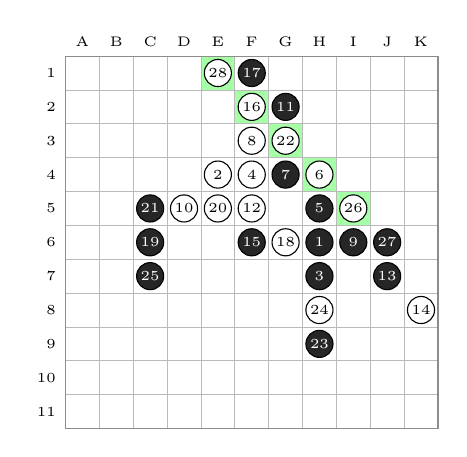
\begin{tikzpicture}[x=0.43cm, y=0.43cm]
\fill[green!35] (4,0) rectangle (5,-1);
\fill[green!35] (5,-1) rectangle (6,-2);
\fill[green!35] (6,-2) rectangle (7,-3);
\fill[green!35] (7,-3) rectangle (8,-4);
\fill[green!35] (8,-4) rectangle (9,-5);
\draw[gray!55, line width=.3pt, step=1] (0,0) grid (11,-11);
\draw[gray!90] (0,0) rectangle (11,-11);
\node[font=\tiny, anchor=south] at (0.5,0) {A};
\node[font=\tiny, anchor=south] at (1.5,0) {B};
\node[font=\tiny, anchor=south] at (2.5,0) {C};
\node[font=\tiny, anchor=south] at (3.5,0) {D};
\node[font=\tiny, anchor=south] at (4.5,0) {E};
\node[font=\tiny, anchor=south] at (5.5,0) {F};
\node[font=\tiny, anchor=south] at (6.5,0) {G};
\node[font=\tiny, anchor=south] at (7.5,0) {H};
\node[font=\tiny, anchor=south] at (8.5,0) {I};
\node[font=\tiny, anchor=south] at (9.5,0) {J};
\node[font=\tiny, anchor=south] at (10.5,0) {K};
\node[font=\tiny, anchor=east] at (0,-0.5) {1};
\node[font=\tiny, anchor=east] at (0,-1.5) {2};
\node[font=\tiny, anchor=east] at (0,-2.5) {3};
\node[font=\tiny, anchor=east] at (0,-3.5) {4};
\node[font=\tiny, anchor=east] at (0,-4.5) {5};
\node[font=\tiny, anchor=east] at (0,-5.5) {6};
\node[font=\tiny, anchor=east] at (0,-6.5) {7};
\node[font=\tiny, anchor=east] at (0,-7.5) {8};
\node[font=\tiny, anchor=east] at (0,-8.5) {9};
\node[font=\tiny, anchor=east] at (0,-9.5) {10};
\node[font=\tiny, anchor=east] at (0,-10.5) {11};
\draw[fill=white, line width=.4pt] (4.5,-0.5) circle (.40);
\node[font=\tiny, text=black, inner sep=0pt] at (4.5,-0.5) {28};
\draw[fill=black!85, line width=.4pt] (5.5,-0.5) circle (.40);
\node[font=\tiny, text=white, inner sep=0pt] at (5.5,-0.5) {17};
\draw[fill=white, line width=.4pt] (5.5,-1.5) circle (.40);
\node[font=\tiny, text=black, inner sep=0pt] at (5.5,-1.5) {16};
\draw[fill=black!85, line width=.4pt] (6.5,-1.5) circle (.40);
\node[font=\tiny, text=white, inner sep=0pt] at (6.5,-1.5) {11};
\draw[fill=white, line width=.4pt] (5.5,-2.5) circle (.40);
\node[font=\tiny, text=black, inner sep=0pt] at (5.5,-2.5) {8};
\draw[fill=white, line width=.4pt] (6.5,-2.5) circle (.40);
\node[font=\tiny, text=black, inner sep=0pt] at (6.5,-2.5) {22};
\draw[fill=white, line width=.4pt] (4.5,-3.5) circle (.40);
\node[font=\tiny, text=black, inner sep=0pt] at (4.5,-3.5) {2};
\draw[fill=white, line width=.4pt] (5.5,-3.5) circle (.40);
\node[font=\tiny, text=black, inner sep=0pt] at (5.5,-3.5) {4};
\draw[fill=black!85, line width=.4pt] (6.5,-3.5) circle (.40);
\node[font=\tiny, text=white, inner sep=0pt] at (6.5,-3.5) {7};
\draw[fill=white, line width=.4pt] (7.5,-3.5) circle (.40);
\node[font=\tiny, text=black, inner sep=0pt] at (7.5,-3.5) {6};
\draw[fill=black!85, line width=.4pt] (2.5,-4.5) circle (.40);
\node[font=\tiny, text=white, inner sep=0pt] at (2.5,-4.5) {21};
\draw[fill=white, line width=.4pt] (3.5,-4.5) circle (.40);
\node[font=\tiny, text=black, inner sep=0pt] at (3.5,-4.5) {10};
\draw[fill=white, line width=.4pt] (4.5,-4.5) circle (.40);
\node[font=\tiny, text=black, inner sep=0pt] at (4.5,-4.5) {20};
\draw[fill=white, line width=.4pt] (5.5,-4.5) circle (.40);
\node[font=\tiny, text=black, inner sep=0pt] at (5.5,-4.5) {12};
\draw[fill=black!85, line width=.4pt] (7.5,-4.5) circle (.40);
\node[font=\tiny, text=white, inner sep=0pt] at (7.5,-4.5) {5};
\draw[fill=white, line width=.4pt] (8.5,-4.5) circle (.40);
\node[font=\tiny, text=black, inner sep=0pt] at (8.5,-4.5) {26};
\draw[fill=black!85, line width=.4pt] (2.5,-5.5) circle (.40);
\node[font=\tiny, text=white, inner sep=0pt] at (2.5,-5.5) {19};
\draw[fill=black!85, line width=.4pt] (5.5,-5.5) circle (.40);
\node[font=\tiny, text=white, inner sep=0pt] at (5.5,-5.5) {15};
\draw[fill=white, line width=.4pt] (6.5,-5.5) circle (.40);
\node[font=\tiny, text=black, inner sep=0pt] at (6.5,-5.5) {18};
\draw[fill=black!85, line width=.4pt] (7.5,-5.5) circle (.40);
\node[font=\tiny, text=white, inner sep=0pt] at (7.5,-5.5) {1};
\draw[fill=black!85, line width=.4pt] (8.5,-5.5) circle (.40);
\node[font=\tiny, text=white, inner sep=0pt] at (8.5,-5.5) {9};
\draw[fill=black!85, line width=.4pt] (9.5,-5.5) circle (.40);
\node[font=\tiny, text=white, inner sep=0pt] at (9.5,-5.5) {27};
\draw[fill=black!85, line width=.4pt] (2.5,-6.5) circle (.40);
\node[font=\tiny, text=white, inner sep=0pt] at (2.5,-6.5) {25};
\draw[fill=black!85, line width=.4pt] (7.5,-6.5) circle (.40);
\node[font=\tiny, text=white, inner sep=0pt] at (7.5,-6.5) {3};
\draw[fill=black!85, line width=.4pt] (9.5,-6.5) circle (.40);
\node[font=\tiny, text=white, inner sep=0pt] at (9.5,-6.5) {13};
\draw[fill=white, line width=.4pt] (7.5,-7.5) circle (.40);
\node[font=\tiny, text=black, inner sep=0pt] at (7.5,-7.5) {24};
\draw[fill=white, line width=.4pt] (10.5,-7.5) circle (.40);
\node[font=\tiny, text=black, inner sep=0pt] at (10.5,-7.5) {14};
\draw[fill=black!85, line width=.4pt] (7.5,-8.5) circle (.40);
\node[font=\tiny, text=white, inner sep=0pt] at (7.5,-8.5) {23};
\end{tikzpicture}
    \caption{Thế cuối (ô xanh: dãy thắng)}
  \end{subfigure}
  \caption{Ván 1600 (L3 cầm X, L7 cầm O).}
  \label{fig:cs-van-17}
\end{figure}
{\footnotesize\linespread{1}\selectfont
\noindent\begin{tabularx}{\linewidth}{*{6}{X}}
\toprule
1.~X H6$^\ast$ & 6.~O H4 & 11.~X G2 & 16.~O F2 & 21.~X C5 & 26.~O I5 \\
2.~O E4$^\ast$ & 7.~X G4 & 12.~O F5 & 17.~X F1 & 22.~O G3 & 27.~X J6 \\
3.~X H7$^\ast$ & 8.~O F3 & 13.~X J7 & 18.~O G6 & 23.~X H9 & 28.~O E1 \\
4.~O F4 & 9.~X I6 & 14.~O K8 & 19.~X C6 & 24.~O H8 &  \\
5.~X H5 & 10.~O D5 & 15.~X F6 & 20.~O E5 & 25.~X C7 &  \\
\bottomrule
\end{tabularx}\par}
\paragraph{Diễn biến chiến thuật.}
\begin{itemize}\small
\setlength{\itemsep}{0pt}
  \item Nước 14 (O=L7, K8): chặn ô thắng K8.
  \item Nước 17 (X=L3, F1): chặn ô thắng F1.
  \item Nước 24 (O=L7, H8): chặn ô thắng H8.
  \item Nước 25 (X=L3, C7): không còn nước nào ngăn được VCF của đối thủ.
  \item Nước 26 (O=L7, I5): đang có VCF 2 nước và đi đúng một đường (H2--I1--D6 là đường ngắn nhất).
  \item Nước 27 (X=L3, J6): đối thủ đang có các ô thắng E1, J6, không đỡ hết được.
  \item Nước 28 (O=L7, E1): thắng ngay.
\end{itemize}
Thời gian trung vị mỗi nước: X 4,8 ms, O 87,5 ms.
\clearpage

\subsection{L3 -- L8: ván 1749}
\label{sec:cs-van-18}
X: \texttt{L8-AlphaZero}; O: \texttt{L3-AlphaBeta}; khai cuộc 24 (4 nước, đánh dấu $\ast$); 27 nước; kết quả: X (L8) thắng. Cả cặp: L3 thắng 11, hoà 13, thua 76 trên 100 ván; trung vị 28 nước.
\begin{figure}[H]
  \centering
  \begin{subfigure}[t]{.48\linewidth}
    \centering
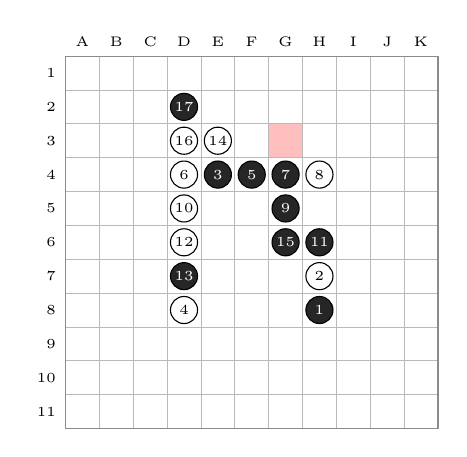
\begin{tikzpicture}[x=0.43cm, y=0.43cm]
\fill[red!25] (6,-2) rectangle (7,-3);
\draw[gray!55, line width=.3pt, step=1] (0,0) grid (11,-11);
\draw[gray!90] (0,0) rectangle (11,-11);
\node[font=\tiny, anchor=south] at (0.5,0) {A};
\node[font=\tiny, anchor=south] at (1.5,0) {B};
\node[font=\tiny, anchor=south] at (2.5,0) {C};
\node[font=\tiny, anchor=south] at (3.5,0) {D};
\node[font=\tiny, anchor=south] at (4.5,0) {E};
\node[font=\tiny, anchor=south] at (5.5,0) {F};
\node[font=\tiny, anchor=south] at (6.5,0) {G};
\node[font=\tiny, anchor=south] at (7.5,0) {H};
\node[font=\tiny, anchor=south] at (8.5,0) {I};
\node[font=\tiny, anchor=south] at (9.5,0) {J};
\node[font=\tiny, anchor=south] at (10.5,0) {K};
\node[font=\tiny, anchor=east] at (0,-0.5) {1};
\node[font=\tiny, anchor=east] at (0,-1.5) {2};
\node[font=\tiny, anchor=east] at (0,-2.5) {3};
\node[font=\tiny, anchor=east] at (0,-3.5) {4};
\node[font=\tiny, anchor=east] at (0,-4.5) {5};
\node[font=\tiny, anchor=east] at (0,-5.5) {6};
\node[font=\tiny, anchor=east] at (0,-6.5) {7};
\node[font=\tiny, anchor=east] at (0,-7.5) {8};
\node[font=\tiny, anchor=east] at (0,-8.5) {9};
\node[font=\tiny, anchor=east] at (0,-9.5) {10};
\node[font=\tiny, anchor=east] at (0,-10.5) {11};
\draw[fill=black!85, line width=.4pt] (3.5,-1.5) circle (.40);
\node[font=\tiny, text=white, inner sep=0pt] at (3.5,-1.5) {17};
\draw[fill=white, line width=.4pt] (3.5,-2.5) circle (.40);
\node[font=\tiny, text=black, inner sep=0pt] at (3.5,-2.5) {16};
\draw[fill=white, line width=.4pt] (4.5,-2.5) circle (.40);
\node[font=\tiny, text=black, inner sep=0pt] at (4.5,-2.5) {14};
\draw[fill=white, line width=.4pt] (3.5,-3.5) circle (.40);
\node[font=\tiny, text=black, inner sep=0pt] at (3.5,-3.5) {6};
\draw[fill=black!85, line width=.4pt] (4.5,-3.5) circle (.40);
\node[font=\tiny, text=white, inner sep=0pt] at (4.5,-3.5) {3};
\draw[fill=black!85, line width=.4pt] (5.5,-3.5) circle (.40);
\node[font=\tiny, text=white, inner sep=0pt] at (5.5,-3.5) {5};
\draw[fill=black!85, line width=.4pt] (6.5,-3.5) circle (.40);
\node[font=\tiny, text=white, inner sep=0pt] at (6.5,-3.5) {7};
\draw[fill=white, line width=.4pt] (7.5,-3.5) circle (.40);
\node[font=\tiny, text=black, inner sep=0pt] at (7.5,-3.5) {8};
\draw[fill=white, line width=.4pt] (3.5,-4.5) circle (.40);
\node[font=\tiny, text=black, inner sep=0pt] at (3.5,-4.5) {10};
\draw[fill=black!85, line width=.4pt] (6.5,-4.5) circle (.40);
\node[font=\tiny, text=white, inner sep=0pt] at (6.5,-4.5) {9};
\draw[fill=white, line width=.4pt] (3.5,-5.5) circle (.40);
\node[font=\tiny, text=black, inner sep=0pt] at (3.5,-5.5) {12};
\draw[fill=black!85, line width=.4pt] (6.5,-5.5) circle (.40);
\node[font=\tiny, text=white, inner sep=0pt] at (6.5,-5.5) {15};
\draw[fill=black!85, line width=.4pt] (7.5,-5.5) circle (.40);
\node[font=\tiny, text=white, inner sep=0pt] at (7.5,-5.5) {11};
\draw[fill=black!85, line width=.4pt] (3.5,-6.5) circle (.40);
\node[font=\tiny, text=white, inner sep=0pt] at (3.5,-6.5) {13};
\draw[fill=white, line width=.4pt] (7.5,-6.5) circle (.40);
\node[font=\tiny, text=black, inner sep=0pt] at (7.5,-6.5) {2};
\draw[fill=white, line width=.4pt] (3.5,-7.5) circle (.40);
\node[font=\tiny, text=black, inner sep=0pt] at (3.5,-7.5) {4};
\draw[fill=black!85, line width=.4pt] (7.5,-7.5) circle (.40);
\node[font=\tiny, text=white, inner sep=0pt] at (7.5,-7.5) {1};
\end{tikzpicture}
    \caption{Trước nước 18 (O đi; ô đỏ là nước đã chọn)}
  \end{subfigure}\hfill
  \begin{subfigure}[t]{.48\linewidth}
    \centering
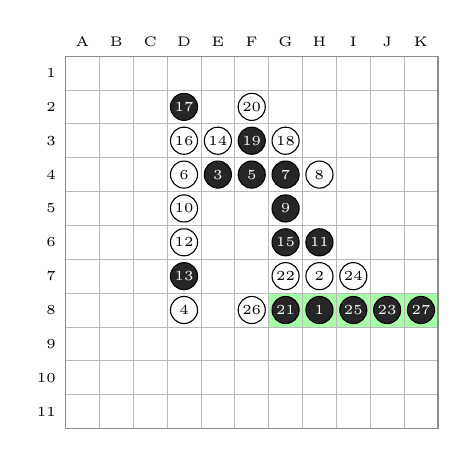
\begin{tikzpicture}[x=0.43cm, y=0.43cm]
\fill[green!35] (10,-7) rectangle (11,-8);
\fill[green!35] (9,-7) rectangle (10,-8);
\fill[green!35] (8,-7) rectangle (9,-8);
\fill[green!35] (7,-7) rectangle (8,-8);
\fill[green!35] (6,-7) rectangle (7,-8);
\draw[gray!55, line width=.3pt, step=1] (0,0) grid (11,-11);
\draw[gray!90] (0,0) rectangle (11,-11);
\node[font=\tiny, anchor=south] at (0.5,0) {A};
\node[font=\tiny, anchor=south] at (1.5,0) {B};
\node[font=\tiny, anchor=south] at (2.5,0) {C};
\node[font=\tiny, anchor=south] at (3.5,0) {D};
\node[font=\tiny, anchor=south] at (4.5,0) {E};
\node[font=\tiny, anchor=south] at (5.5,0) {F};
\node[font=\tiny, anchor=south] at (6.5,0) {G};
\node[font=\tiny, anchor=south] at (7.5,0) {H};
\node[font=\tiny, anchor=south] at (8.5,0) {I};
\node[font=\tiny, anchor=south] at (9.5,0) {J};
\node[font=\tiny, anchor=south] at (10.5,0) {K};
\node[font=\tiny, anchor=east] at (0,-0.5) {1};
\node[font=\tiny, anchor=east] at (0,-1.5) {2};
\node[font=\tiny, anchor=east] at (0,-2.5) {3};
\node[font=\tiny, anchor=east] at (0,-3.5) {4};
\node[font=\tiny, anchor=east] at (0,-4.5) {5};
\node[font=\tiny, anchor=east] at (0,-5.5) {6};
\node[font=\tiny, anchor=east] at (0,-6.5) {7};
\node[font=\tiny, anchor=east] at (0,-7.5) {8};
\node[font=\tiny, anchor=east] at (0,-8.5) {9};
\node[font=\tiny, anchor=east] at (0,-9.5) {10};
\node[font=\tiny, anchor=east] at (0,-10.5) {11};
\draw[fill=black!85, line width=.4pt] (3.5,-1.5) circle (.40);
\node[font=\tiny, text=white, inner sep=0pt] at (3.5,-1.5) {17};
\draw[fill=white, line width=.4pt] (5.5,-1.5) circle (.40);
\node[font=\tiny, text=black, inner sep=0pt] at (5.5,-1.5) {20};
\draw[fill=white, line width=.4pt] (3.5,-2.5) circle (.40);
\node[font=\tiny, text=black, inner sep=0pt] at (3.5,-2.5) {16};
\draw[fill=white, line width=.4pt] (4.5,-2.5) circle (.40);
\node[font=\tiny, text=black, inner sep=0pt] at (4.5,-2.5) {14};
\draw[fill=black!85, line width=.4pt] (5.5,-2.5) circle (.40);
\node[font=\tiny, text=white, inner sep=0pt] at (5.5,-2.5) {19};
\draw[fill=white, line width=.4pt] (6.5,-2.5) circle (.40);
\node[font=\tiny, text=black, inner sep=0pt] at (6.5,-2.5) {18};
\draw[fill=white, line width=.4pt] (3.5,-3.5) circle (.40);
\node[font=\tiny, text=black, inner sep=0pt] at (3.5,-3.5) {6};
\draw[fill=black!85, line width=.4pt] (4.5,-3.5) circle (.40);
\node[font=\tiny, text=white, inner sep=0pt] at (4.5,-3.5) {3};
\draw[fill=black!85, line width=.4pt] (5.5,-3.5) circle (.40);
\node[font=\tiny, text=white, inner sep=0pt] at (5.5,-3.5) {5};
\draw[fill=black!85, line width=.4pt] (6.5,-3.5) circle (.40);
\node[font=\tiny, text=white, inner sep=0pt] at (6.5,-3.5) {7};
\draw[fill=white, line width=.4pt] (7.5,-3.5) circle (.40);
\node[font=\tiny, text=black, inner sep=0pt] at (7.5,-3.5) {8};
\draw[fill=white, line width=.4pt] (3.5,-4.5) circle (.40);
\node[font=\tiny, text=black, inner sep=0pt] at (3.5,-4.5) {10};
\draw[fill=black!85, line width=.4pt] (6.5,-4.5) circle (.40);
\node[font=\tiny, text=white, inner sep=0pt] at (6.5,-4.5) {9};
\draw[fill=white, line width=.4pt] (3.5,-5.5) circle (.40);
\node[font=\tiny, text=black, inner sep=0pt] at (3.5,-5.5) {12};
\draw[fill=black!85, line width=.4pt] (6.5,-5.5) circle (.40);
\node[font=\tiny, text=white, inner sep=0pt] at (6.5,-5.5) {15};
\draw[fill=black!85, line width=.4pt] (7.5,-5.5) circle (.40);
\node[font=\tiny, text=white, inner sep=0pt] at (7.5,-5.5) {11};
\draw[fill=black!85, line width=.4pt] (3.5,-6.5) circle (.40);
\node[font=\tiny, text=white, inner sep=0pt] at (3.5,-6.5) {13};
\draw[fill=white, line width=.4pt] (6.5,-6.5) circle (.40);
\node[font=\tiny, text=black, inner sep=0pt] at (6.5,-6.5) {22};
\draw[fill=white, line width=.4pt] (7.5,-6.5) circle (.40);
\node[font=\tiny, text=black, inner sep=0pt] at (7.5,-6.5) {2};
\draw[fill=white, line width=.4pt] (8.5,-6.5) circle (.40);
\node[font=\tiny, text=black, inner sep=0pt] at (8.5,-6.5) {24};
\draw[fill=white, line width=.4pt] (3.5,-7.5) circle (.40);
\node[font=\tiny, text=black, inner sep=0pt] at (3.5,-7.5) {4};
\draw[fill=white, line width=.4pt] (5.5,-7.5) circle (.40);
\node[font=\tiny, text=black, inner sep=0pt] at (5.5,-7.5) {26};
\draw[fill=black!85, line width=.4pt] (6.5,-7.5) circle (.40);
\node[font=\tiny, text=white, inner sep=0pt] at (6.5,-7.5) {21};
\draw[fill=black!85, line width=.4pt] (7.5,-7.5) circle (.40);
\node[font=\tiny, text=white, inner sep=0pt] at (7.5,-7.5) {1};
\draw[fill=black!85, line width=.4pt] (8.5,-7.5) circle (.40);
\node[font=\tiny, text=white, inner sep=0pt] at (8.5,-7.5) {25};
\draw[fill=black!85, line width=.4pt] (9.5,-7.5) circle (.40);
\node[font=\tiny, text=white, inner sep=0pt] at (9.5,-7.5) {23};
\draw[fill=black!85, line width=.4pt] (10.5,-7.5) circle (.40);
\node[font=\tiny, text=white, inner sep=0pt] at (10.5,-7.5) {27};
\end{tikzpicture}
    \caption{Thế cuối (ô xanh: dãy thắng)}
  \end{subfigure}
  \caption{Ván 1749 (L8 cầm X, L3 cầm O).}
  \label{fig:cs-van-18}
\end{figure}
{\footnotesize\linespread{1}\selectfont
\noindent\begin{tabularx}{\linewidth}{*{6}{X}}
\toprule
1.~X H8$^\ast$ & 6.~O D4 & 11.~X H6 & 16.~O D3 & 21.~X G8 & 26.~O F8 \\
2.~O H7$^\ast$ & 7.~X G4 & 12.~O D6 & 17.~X D2 & 22.~O G7 & 27.~X K8 \\
3.~X E4$^\ast$ & 8.~O H4 & 13.~X D7 & 18.~O G3 & 23.~X J8 &  \\
4.~O D8$^\ast$ & 9.~X G5 & 14.~O E3 & 19.~X F3 & 24.~O I7 &  \\
5.~X F4 & 10.~O D5 & 15.~X G6 & 20.~O F2 & 25.~X I8 &  \\
\bottomrule
\end{tabularx}\par}
\paragraph{Diễn biến chiến thuật.}
\begin{itemize}\small
\setlength{\itemsep}{0pt}
  \item Nước 13 (X=L8, D7): chặn ô thắng D7.
  \item Nước 17 (X=L8, D2): chặn ô thắng D2.
  \item Nước 18 (O=L3, G3): để đối thủ có VCF: G8--G7--J8--I7--I8--F8--K8.
  \item Nước 19 (X=L8, F3): bỏ lỡ VCF 4 nước: G8--G7--J8--I7--I8--F8--K8.
  \item Nước 20 (O=L3, F2): để đối thủ có VCF: G8--G7--J8--I7--I8--F8--K8.
  \item Nước 21 (X=L8, G8): đang có VCF 4 nước và đi đúng một đường (G8--G7--J8--I7--I8--F8--K8 là đường ngắn nhất).
  \item Nước 22 (O=L3, G7): chặn ô thắng G7.
  \item Nước 23 (X=L8, J8): đang có VCF 3 nước và đi đúng một đường (J8--I7--I8--F8--K8 là đường ngắn nhất).
  \item Nước 24 (O=L3, I7): chặn ô thắng I7.
  \item Nước 25 (X=L8, I8): đang có VCF 2 nước và đi đúng một đường (I8--F8--K8 là đường ngắn nhất).
  \item Nước 26 (O=L3, F8): đối thủ đang có các ô thắng F8, K8, không đỡ hết được.
  \item Nước 27 (X=L8, K8): thắng ngay.
\end{itemize}
Thời gian trung vị mỗi nước: X 86,3 ms, O 5,2 ms.
\clearpage

\subsection{L4 -- L5: ván 1819}
\label{sec:cs-van-19}
X: \texttt{L5-PolicySL}; O: \texttt{L4-MCTS}; khai cuộc 9 (4 nước, đánh dấu $\ast$); 11 nước; kết quả: X (L5) thắng. Cả cặp: L4 thắng 0, hoà 0, thua 100 trên 100 ván; trung vị 11 nước.
\begin{figure}[H]
  \centering
  \begin{subfigure}[t]{.48\linewidth}
    \centering
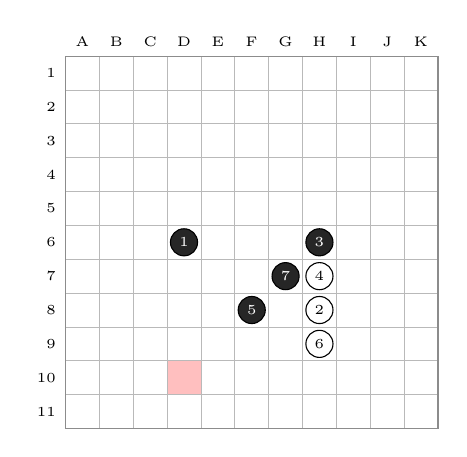
\begin{tikzpicture}[x=0.43cm, y=0.43cm]
\fill[red!25] (3,-9) rectangle (4,-10);
\draw[gray!55, line width=.3pt, step=1] (0,0) grid (11,-11);
\draw[gray!90] (0,0) rectangle (11,-11);
\node[font=\tiny, anchor=south] at (0.5,0) {A};
\node[font=\tiny, anchor=south] at (1.5,0) {B};
\node[font=\tiny, anchor=south] at (2.5,0) {C};
\node[font=\tiny, anchor=south] at (3.5,0) {D};
\node[font=\tiny, anchor=south] at (4.5,0) {E};
\node[font=\tiny, anchor=south] at (5.5,0) {F};
\node[font=\tiny, anchor=south] at (6.5,0) {G};
\node[font=\tiny, anchor=south] at (7.5,0) {H};
\node[font=\tiny, anchor=south] at (8.5,0) {I};
\node[font=\tiny, anchor=south] at (9.5,0) {J};
\node[font=\tiny, anchor=south] at (10.5,0) {K};
\node[font=\tiny, anchor=east] at (0,-0.5) {1};
\node[font=\tiny, anchor=east] at (0,-1.5) {2};
\node[font=\tiny, anchor=east] at (0,-2.5) {3};
\node[font=\tiny, anchor=east] at (0,-3.5) {4};
\node[font=\tiny, anchor=east] at (0,-4.5) {5};
\node[font=\tiny, anchor=east] at (0,-5.5) {6};
\node[font=\tiny, anchor=east] at (0,-6.5) {7};
\node[font=\tiny, anchor=east] at (0,-7.5) {8};
\node[font=\tiny, anchor=east] at (0,-8.5) {9};
\node[font=\tiny, anchor=east] at (0,-9.5) {10};
\node[font=\tiny, anchor=east] at (0,-10.5) {11};
\draw[fill=black!85, line width=.4pt] (3.5,-5.5) circle (.40);
\node[font=\tiny, text=white, inner sep=0pt] at (3.5,-5.5) {1};
\draw[fill=black!85, line width=.4pt] (7.5,-5.5) circle (.40);
\node[font=\tiny, text=white, inner sep=0pt] at (7.5,-5.5) {3};
\draw[fill=black!85, line width=.4pt] (6.5,-6.5) circle (.40);
\node[font=\tiny, text=white, inner sep=0pt] at (6.5,-6.5) {7};
\draw[fill=white, line width=.4pt] (7.5,-6.5) circle (.40);
\node[font=\tiny, text=black, inner sep=0pt] at (7.5,-6.5) {4};
\draw[fill=black!85, line width=.4pt] (5.5,-7.5) circle (.40);
\node[font=\tiny, text=white, inner sep=0pt] at (5.5,-7.5) {5};
\draw[fill=white, line width=.4pt] (7.5,-7.5) circle (.40);
\node[font=\tiny, text=black, inner sep=0pt] at (7.5,-7.5) {2};
\draw[fill=white, line width=.4pt] (7.5,-8.5) circle (.40);
\node[font=\tiny, text=black, inner sep=0pt] at (7.5,-8.5) {6};
\end{tikzpicture}
    \caption{Trước nước 8 (O đi; ô đỏ là nước đã chọn)}
  \end{subfigure}\hfill
  \begin{subfigure}[t]{.48\linewidth}
    \centering
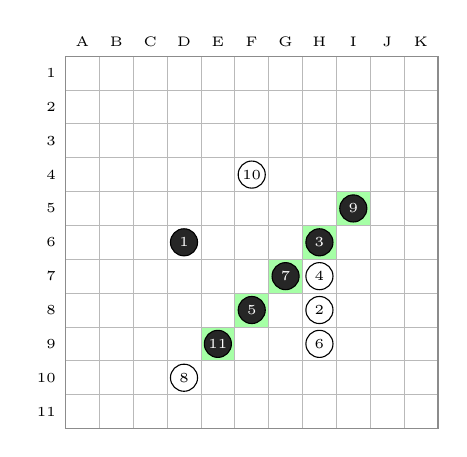
\begin{tikzpicture}[x=0.43cm, y=0.43cm]
\fill[green!35] (4,-8) rectangle (5,-9);
\fill[green!35] (5,-7) rectangle (6,-8);
\fill[green!35] (6,-6) rectangle (7,-7);
\fill[green!35] (7,-5) rectangle (8,-6);
\fill[green!35] (8,-4) rectangle (9,-5);
\draw[gray!55, line width=.3pt, step=1] (0,0) grid (11,-11);
\draw[gray!90] (0,0) rectangle (11,-11);
\node[font=\tiny, anchor=south] at (0.5,0) {A};
\node[font=\tiny, anchor=south] at (1.5,0) {B};
\node[font=\tiny, anchor=south] at (2.5,0) {C};
\node[font=\tiny, anchor=south] at (3.5,0) {D};
\node[font=\tiny, anchor=south] at (4.5,0) {E};
\node[font=\tiny, anchor=south] at (5.5,0) {F};
\node[font=\tiny, anchor=south] at (6.5,0) {G};
\node[font=\tiny, anchor=south] at (7.5,0) {H};
\node[font=\tiny, anchor=south] at (8.5,0) {I};
\node[font=\tiny, anchor=south] at (9.5,0) {J};
\node[font=\tiny, anchor=south] at (10.5,0) {K};
\node[font=\tiny, anchor=east] at (0,-0.5) {1};
\node[font=\tiny, anchor=east] at (0,-1.5) {2};
\node[font=\tiny, anchor=east] at (0,-2.5) {3};
\node[font=\tiny, anchor=east] at (0,-3.5) {4};
\node[font=\tiny, anchor=east] at (0,-4.5) {5};
\node[font=\tiny, anchor=east] at (0,-5.5) {6};
\node[font=\tiny, anchor=east] at (0,-6.5) {7};
\node[font=\tiny, anchor=east] at (0,-7.5) {8};
\node[font=\tiny, anchor=east] at (0,-8.5) {9};
\node[font=\tiny, anchor=east] at (0,-9.5) {10};
\node[font=\tiny, anchor=east] at (0,-10.5) {11};
\draw[fill=white, line width=.4pt] (5.5,-3.5) circle (.40);
\node[font=\tiny, text=black, inner sep=0pt] at (5.5,-3.5) {10};
\draw[fill=black!85, line width=.4pt] (8.5,-4.5) circle (.40);
\node[font=\tiny, text=white, inner sep=0pt] at (8.5,-4.5) {9};
\draw[fill=black!85, line width=.4pt] (3.5,-5.5) circle (.40);
\node[font=\tiny, text=white, inner sep=0pt] at (3.5,-5.5) {1};
\draw[fill=black!85, line width=.4pt] (7.5,-5.5) circle (.40);
\node[font=\tiny, text=white, inner sep=0pt] at (7.5,-5.5) {3};
\draw[fill=black!85, line width=.4pt] (6.5,-6.5) circle (.40);
\node[font=\tiny, text=white, inner sep=0pt] at (6.5,-6.5) {7};
\draw[fill=white, line width=.4pt] (7.5,-6.5) circle (.40);
\node[font=\tiny, text=black, inner sep=0pt] at (7.5,-6.5) {4};
\draw[fill=black!85, line width=.4pt] (5.5,-7.5) circle (.40);
\node[font=\tiny, text=white, inner sep=0pt] at (5.5,-7.5) {5};
\draw[fill=white, line width=.4pt] (7.5,-7.5) circle (.40);
\node[font=\tiny, text=black, inner sep=0pt] at (7.5,-7.5) {2};
\draw[fill=black!85, line width=.4pt] (4.5,-8.5) circle (.40);
\node[font=\tiny, text=white, inner sep=0pt] at (4.5,-8.5) {11};
\draw[fill=white, line width=.4pt] (7.5,-8.5) circle (.40);
\node[font=\tiny, text=black, inner sep=0pt] at (7.5,-8.5) {6};
\draw[fill=white, line width=.4pt] (3.5,-9.5) circle (.40);
\node[font=\tiny, text=black, inner sep=0pt] at (3.5,-9.5) {8};
\end{tikzpicture}
    \caption{Thế cuối (ô xanh: dãy thắng)}
  \end{subfigure}
  \caption{Ván 1819 (L5 cầm X, L4 cầm O).}
  \label{fig:cs-van-19}
\end{figure}
{\footnotesize\linespread{1}\selectfont
\noindent\begin{tabularx}{\linewidth}{*{6}{X}}
\toprule
1.~X D6$^\ast$ & 3.~X H6$^\ast$ & 5.~X F8 & 7.~X G7 & 9.~X I5 & 11.~X E9 \\
2.~O H8$^\ast$ & 4.~O H7$^\ast$ & 6.~O H9 & 8.~O D10 & 10.~O F4 &  \\
\bottomrule
\end{tabularx}\par}
\paragraph{Diễn biến chiến thuật.}
\begin{itemize}\small
\setlength{\itemsep}{0pt}
  \item Nước 8 (O=L4, D10): để đối thủ có VCF: I5--J4--E9.
  \item Nước 9 (X=L5, I5): đang có VCF 2 nước và đi đúng một đường (I5--J4--E9 là đường ngắn nhất).
  \item Nước 10 (O=L4, F4): đối thủ đang có các ô thắng J4, E9, không đỡ hết được.
  \item Nước 11 (X=L5, E9): thắng ngay.
\end{itemize}
Thời gian trung vị mỗi nước: X 1,3 ms, O 55,5 ms.
\clearpage

\subsection{L4 -- L6: ván 1912}
\label{sec:cs-van-20}
X: \texttt{L4-MCTS}; O: \texttt{L6-PolicyRL}; khai cuộc 6 (3 nước, đánh dấu $\ast$); 12 nước; kết quả: O (L6) thắng. Cả cặp: L4 thắng 0, hoà 0, thua 100 trên 100 ván; trung vị 12 nước.
\begin{figure}[H]
  \centering
  \begin{subfigure}[t]{.48\linewidth}
    \centering
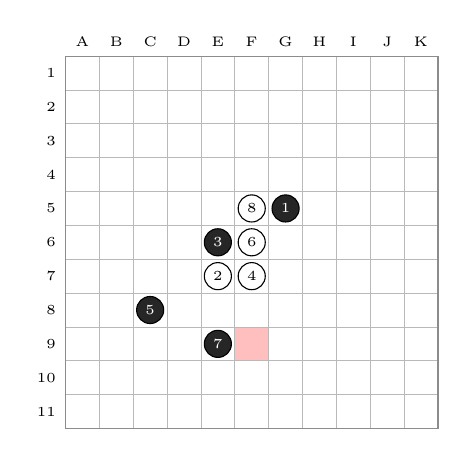
\begin{tikzpicture}[x=0.43cm, y=0.43cm]
\fill[red!25] (5,-8) rectangle (6,-9);
\draw[gray!55, line width=.3pt, step=1] (0,0) grid (11,-11);
\draw[gray!90] (0,0) rectangle (11,-11);
\node[font=\tiny, anchor=south] at (0.5,0) {A};
\node[font=\tiny, anchor=south] at (1.5,0) {B};
\node[font=\tiny, anchor=south] at (2.5,0) {C};
\node[font=\tiny, anchor=south] at (3.5,0) {D};
\node[font=\tiny, anchor=south] at (4.5,0) {E};
\node[font=\tiny, anchor=south] at (5.5,0) {F};
\node[font=\tiny, anchor=south] at (6.5,0) {G};
\node[font=\tiny, anchor=south] at (7.5,0) {H};
\node[font=\tiny, anchor=south] at (8.5,0) {I};
\node[font=\tiny, anchor=south] at (9.5,0) {J};
\node[font=\tiny, anchor=south] at (10.5,0) {K};
\node[font=\tiny, anchor=east] at (0,-0.5) {1};
\node[font=\tiny, anchor=east] at (0,-1.5) {2};
\node[font=\tiny, anchor=east] at (0,-2.5) {3};
\node[font=\tiny, anchor=east] at (0,-3.5) {4};
\node[font=\tiny, anchor=east] at (0,-4.5) {5};
\node[font=\tiny, anchor=east] at (0,-5.5) {6};
\node[font=\tiny, anchor=east] at (0,-6.5) {7};
\node[font=\tiny, anchor=east] at (0,-7.5) {8};
\node[font=\tiny, anchor=east] at (0,-8.5) {9};
\node[font=\tiny, anchor=east] at (0,-9.5) {10};
\node[font=\tiny, anchor=east] at (0,-10.5) {11};
\draw[fill=white, line width=.4pt] (5.5,-4.5) circle (.40);
\node[font=\tiny, text=black, inner sep=0pt] at (5.5,-4.5) {8};
\draw[fill=black!85, line width=.4pt] (6.5,-4.5) circle (.40);
\node[font=\tiny, text=white, inner sep=0pt] at (6.5,-4.5) {1};
\draw[fill=black!85, line width=.4pt] (4.5,-5.5) circle (.40);
\node[font=\tiny, text=white, inner sep=0pt] at (4.5,-5.5) {3};
\draw[fill=white, line width=.4pt] (5.5,-5.5) circle (.40);
\node[font=\tiny, text=black, inner sep=0pt] at (5.5,-5.5) {6};
\draw[fill=white, line width=.4pt] (4.5,-6.5) circle (.40);
\node[font=\tiny, text=black, inner sep=0pt] at (4.5,-6.5) {2};
\draw[fill=white, line width=.4pt] (5.5,-6.5) circle (.40);
\node[font=\tiny, text=black, inner sep=0pt] at (5.5,-6.5) {4};
\draw[fill=black!85, line width=.4pt] (2.5,-7.5) circle (.40);
\node[font=\tiny, text=white, inner sep=0pt] at (2.5,-7.5) {5};
\draw[fill=black!85, line width=.4pt] (4.5,-8.5) circle (.40);
\node[font=\tiny, text=white, inner sep=0pt] at (4.5,-8.5) {7};
\end{tikzpicture}
    \caption{Trước nước 9 (X đi; ô đỏ là nước đã chọn)}
  \end{subfigure}\hfill
  \begin{subfigure}[t]{.48\linewidth}
    \centering
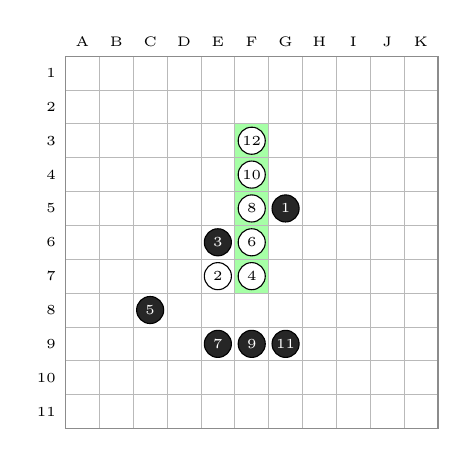
\begin{tikzpicture}[x=0.43cm, y=0.43cm]
\fill[green!35] (5,-2) rectangle (6,-3);
\fill[green!35] (5,-3) rectangle (6,-4);
\fill[green!35] (5,-4) rectangle (6,-5);
\fill[green!35] (5,-5) rectangle (6,-6);
\fill[green!35] (5,-6) rectangle (6,-7);
\draw[gray!55, line width=.3pt, step=1] (0,0) grid (11,-11);
\draw[gray!90] (0,0) rectangle (11,-11);
\node[font=\tiny, anchor=south] at (0.5,0) {A};
\node[font=\tiny, anchor=south] at (1.5,0) {B};
\node[font=\tiny, anchor=south] at (2.5,0) {C};
\node[font=\tiny, anchor=south] at (3.5,0) {D};
\node[font=\tiny, anchor=south] at (4.5,0) {E};
\node[font=\tiny, anchor=south] at (5.5,0) {F};
\node[font=\tiny, anchor=south] at (6.5,0) {G};
\node[font=\tiny, anchor=south] at (7.5,0) {H};
\node[font=\tiny, anchor=south] at (8.5,0) {I};
\node[font=\tiny, anchor=south] at (9.5,0) {J};
\node[font=\tiny, anchor=south] at (10.5,0) {K};
\node[font=\tiny, anchor=east] at (0,-0.5) {1};
\node[font=\tiny, anchor=east] at (0,-1.5) {2};
\node[font=\tiny, anchor=east] at (0,-2.5) {3};
\node[font=\tiny, anchor=east] at (0,-3.5) {4};
\node[font=\tiny, anchor=east] at (0,-4.5) {5};
\node[font=\tiny, anchor=east] at (0,-5.5) {6};
\node[font=\tiny, anchor=east] at (0,-6.5) {7};
\node[font=\tiny, anchor=east] at (0,-7.5) {8};
\node[font=\tiny, anchor=east] at (0,-8.5) {9};
\node[font=\tiny, anchor=east] at (0,-9.5) {10};
\node[font=\tiny, anchor=east] at (0,-10.5) {11};
\draw[fill=white, line width=.4pt] (5.5,-2.5) circle (.40);
\node[font=\tiny, text=black, inner sep=0pt] at (5.5,-2.5) {12};
\draw[fill=white, line width=.4pt] (5.5,-3.5) circle (.40);
\node[font=\tiny, text=black, inner sep=0pt] at (5.5,-3.5) {10};
\draw[fill=white, line width=.4pt] (5.5,-4.5) circle (.40);
\node[font=\tiny, text=black, inner sep=0pt] at (5.5,-4.5) {8};
\draw[fill=black!85, line width=.4pt] (6.5,-4.5) circle (.40);
\node[font=\tiny, text=white, inner sep=0pt] at (6.5,-4.5) {1};
\draw[fill=black!85, line width=.4pt] (4.5,-5.5) circle (.40);
\node[font=\tiny, text=white, inner sep=0pt] at (4.5,-5.5) {3};
\draw[fill=white, line width=.4pt] (5.5,-5.5) circle (.40);
\node[font=\tiny, text=black, inner sep=0pt] at (5.5,-5.5) {6};
\draw[fill=white, line width=.4pt] (4.5,-6.5) circle (.40);
\node[font=\tiny, text=black, inner sep=0pt] at (4.5,-6.5) {2};
\draw[fill=white, line width=.4pt] (5.5,-6.5) circle (.40);
\node[font=\tiny, text=black, inner sep=0pt] at (5.5,-6.5) {4};
\draw[fill=black!85, line width=.4pt] (2.5,-7.5) circle (.40);
\node[font=\tiny, text=white, inner sep=0pt] at (2.5,-7.5) {5};
\draw[fill=black!85, line width=.4pt] (4.5,-8.5) circle (.40);
\node[font=\tiny, text=white, inner sep=0pt] at (4.5,-8.5) {7};
\draw[fill=black!85, line width=.4pt] (5.5,-8.5) circle (.40);
\node[font=\tiny, text=white, inner sep=0pt] at (5.5,-8.5) {9};
\draw[fill=black!85, line width=.4pt] (6.5,-8.5) circle (.40);
\node[font=\tiny, text=white, inner sep=0pt] at (6.5,-8.5) {11};
\end{tikzpicture}
    \caption{Thế cuối (ô xanh: dãy thắng)}
  \end{subfigure}
  \caption{Ván 1912 (L4 cầm X, L6 cầm O).}
  \label{fig:cs-van-20}
\end{figure}
{\footnotesize\linespread{1}\selectfont
\noindent\begin{tabularx}{\linewidth}{*{6}{X}}
\toprule
1.~X G5$^\ast$ & 3.~X E6$^\ast$ & 5.~X C8 & 7.~X E9 & 9.~X F9 & 11.~X G9 \\
2.~O E7$^\ast$ & 4.~O F7 & 6.~O F6 & 8.~O F5 & 10.~O F4 & 12.~O F3 \\
\bottomrule
\end{tabularx}\par}
\paragraph{Diễn biến chiến thuật.}
\begin{itemize}\small
\setlength{\itemsep}{0pt}
  \item Nước 9 (X=L4, F9): để đối thủ có VCF: F4--F3--F8.
  \item Nước 10 (O=L6, F4): đang có VCF 2 nước và đi đúng một đường (F4--F3--F8 là đường ngắn nhất).
  \item Nước 11 (X=L4, G9): đối thủ đang có các ô thắng F3, F8, không đỡ hết được.
  \item Nước 12 (O=L6, F3): thắng ngay.
\end{itemize}
Thời gian trung vị mỗi nước: X 58,1 ms, O 1,1 ms.
\clearpage

\subsection{L4 -- L7: ván 2098}
\label{sec:cs-van-21}
X: \texttt{L4-MCTS}; O: \texttt{L7-PUCT}; khai cuộc 49 (3 nước, đánh dấu $\ast$); 10 nước; kết quả: O (L7) thắng. Cả cặp: L4 thắng 0, hoà 0, thua 100 trên 100 ván; trung vị 10 nước.
\begin{figure}[H]
  \centering
  \begin{subfigure}[t]{.48\linewidth}
    \centering
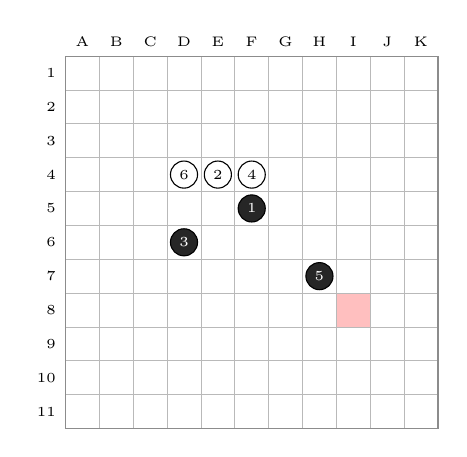
\begin{tikzpicture}[x=0.43cm, y=0.43cm]
\fill[red!25] (8,-7) rectangle (9,-8);
\draw[gray!55, line width=.3pt, step=1] (0,0) grid (11,-11);
\draw[gray!90] (0,0) rectangle (11,-11);
\node[font=\tiny, anchor=south] at (0.5,0) {A};
\node[font=\tiny, anchor=south] at (1.5,0) {B};
\node[font=\tiny, anchor=south] at (2.5,0) {C};
\node[font=\tiny, anchor=south] at (3.5,0) {D};
\node[font=\tiny, anchor=south] at (4.5,0) {E};
\node[font=\tiny, anchor=south] at (5.5,0) {F};
\node[font=\tiny, anchor=south] at (6.5,0) {G};
\node[font=\tiny, anchor=south] at (7.5,0) {H};
\node[font=\tiny, anchor=south] at (8.5,0) {I};
\node[font=\tiny, anchor=south] at (9.5,0) {J};
\node[font=\tiny, anchor=south] at (10.5,0) {K};
\node[font=\tiny, anchor=east] at (0,-0.5) {1};
\node[font=\tiny, anchor=east] at (0,-1.5) {2};
\node[font=\tiny, anchor=east] at (0,-2.5) {3};
\node[font=\tiny, anchor=east] at (0,-3.5) {4};
\node[font=\tiny, anchor=east] at (0,-4.5) {5};
\node[font=\tiny, anchor=east] at (0,-5.5) {6};
\node[font=\tiny, anchor=east] at (0,-6.5) {7};
\node[font=\tiny, anchor=east] at (0,-7.5) {8};
\node[font=\tiny, anchor=east] at (0,-8.5) {9};
\node[font=\tiny, anchor=east] at (0,-9.5) {10};
\node[font=\tiny, anchor=east] at (0,-10.5) {11};
\draw[fill=white, line width=.4pt] (3.5,-3.5) circle (.40);
\node[font=\tiny, text=black, inner sep=0pt] at (3.5,-3.5) {6};
\draw[fill=white, line width=.4pt] (4.5,-3.5) circle (.40);
\node[font=\tiny, text=black, inner sep=0pt] at (4.5,-3.5) {2};
\draw[fill=white, line width=.4pt] (5.5,-3.5) circle (.40);
\node[font=\tiny, text=black, inner sep=0pt] at (5.5,-3.5) {4};
\draw[fill=black!85, line width=.4pt] (5.5,-4.5) circle (.40);
\node[font=\tiny, text=white, inner sep=0pt] at (5.5,-4.5) {1};
\draw[fill=black!85, line width=.4pt] (3.5,-5.5) circle (.40);
\node[font=\tiny, text=white, inner sep=0pt] at (3.5,-5.5) {3};
\draw[fill=black!85, line width=.4pt] (7.5,-6.5) circle (.40);
\node[font=\tiny, text=white, inner sep=0pt] at (7.5,-6.5) {5};
\end{tikzpicture}
    \caption{Trước nước 7 (X đi; ô đỏ là nước đã chọn)}
  \end{subfigure}\hfill
  \begin{subfigure}[t]{.48\linewidth}
    \centering
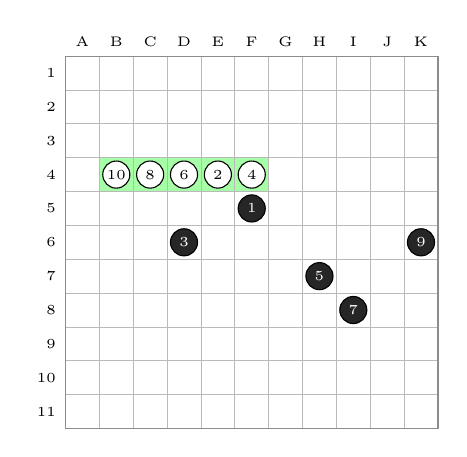
\begin{tikzpicture}[x=0.43cm, y=0.43cm]
\fill[green!35] (1,-3) rectangle (2,-4);
\fill[green!35] (2,-3) rectangle (3,-4);
\fill[green!35] (3,-3) rectangle (4,-4);
\fill[green!35] (4,-3) rectangle (5,-4);
\fill[green!35] (5,-3) rectangle (6,-4);
\draw[gray!55, line width=.3pt, step=1] (0,0) grid (11,-11);
\draw[gray!90] (0,0) rectangle (11,-11);
\node[font=\tiny, anchor=south] at (0.5,0) {A};
\node[font=\tiny, anchor=south] at (1.5,0) {B};
\node[font=\tiny, anchor=south] at (2.5,0) {C};
\node[font=\tiny, anchor=south] at (3.5,0) {D};
\node[font=\tiny, anchor=south] at (4.5,0) {E};
\node[font=\tiny, anchor=south] at (5.5,0) {F};
\node[font=\tiny, anchor=south] at (6.5,0) {G};
\node[font=\tiny, anchor=south] at (7.5,0) {H};
\node[font=\tiny, anchor=south] at (8.5,0) {I};
\node[font=\tiny, anchor=south] at (9.5,0) {J};
\node[font=\tiny, anchor=south] at (10.5,0) {K};
\node[font=\tiny, anchor=east] at (0,-0.5) {1};
\node[font=\tiny, anchor=east] at (0,-1.5) {2};
\node[font=\tiny, anchor=east] at (0,-2.5) {3};
\node[font=\tiny, anchor=east] at (0,-3.5) {4};
\node[font=\tiny, anchor=east] at (0,-4.5) {5};
\node[font=\tiny, anchor=east] at (0,-5.5) {6};
\node[font=\tiny, anchor=east] at (0,-6.5) {7};
\node[font=\tiny, anchor=east] at (0,-7.5) {8};
\node[font=\tiny, anchor=east] at (0,-8.5) {9};
\node[font=\tiny, anchor=east] at (0,-9.5) {10};
\node[font=\tiny, anchor=east] at (0,-10.5) {11};
\draw[fill=white, line width=.4pt] (1.5,-3.5) circle (.40);
\node[font=\tiny, text=black, inner sep=0pt] at (1.5,-3.5) {10};
\draw[fill=white, line width=.4pt] (2.5,-3.5) circle (.40);
\node[font=\tiny, text=black, inner sep=0pt] at (2.5,-3.5) {8};
\draw[fill=white, line width=.4pt] (3.5,-3.5) circle (.40);
\node[font=\tiny, text=black, inner sep=0pt] at (3.5,-3.5) {6};
\draw[fill=white, line width=.4pt] (4.5,-3.5) circle (.40);
\node[font=\tiny, text=black, inner sep=0pt] at (4.5,-3.5) {2};
\draw[fill=white, line width=.4pt] (5.5,-3.5) circle (.40);
\node[font=\tiny, text=black, inner sep=0pt] at (5.5,-3.5) {4};
\draw[fill=black!85, line width=.4pt] (5.5,-4.5) circle (.40);
\node[font=\tiny, text=white, inner sep=0pt] at (5.5,-4.5) {1};
\draw[fill=black!85, line width=.4pt] (3.5,-5.5) circle (.40);
\node[font=\tiny, text=white, inner sep=0pt] at (3.5,-5.5) {3};
\draw[fill=black!85, line width=.4pt] (10.5,-5.5) circle (.40);
\node[font=\tiny, text=white, inner sep=0pt] at (10.5,-5.5) {9};
\draw[fill=black!85, line width=.4pt] (7.5,-6.5) circle (.40);
\node[font=\tiny, text=white, inner sep=0pt] at (7.5,-6.5) {5};
\draw[fill=black!85, line width=.4pt] (8.5,-7.5) circle (.40);
\node[font=\tiny, text=white, inner sep=0pt] at (8.5,-7.5) {7};
\end{tikzpicture}
    \caption{Thế cuối (ô xanh: dãy thắng)}
  \end{subfigure}
  \caption{Ván 2098 (L4 cầm X, L7 cầm O).}
  \label{fig:cs-van-21}
\end{figure}
{\footnotesize\linespread{1}\selectfont
\noindent\begin{tabularx}{\linewidth}{*{6}{X}}
\toprule
1.~X F5$^\ast$ & 3.~X D6$^\ast$ & 5.~X H7 & 7.~X I8 & 9.~X K6 &  \\
2.~O E4$^\ast$ & 4.~O F4 & 6.~O D4 & 8.~O C4 & 10.~O B4 &  \\
\bottomrule
\end{tabularx}\par}
\paragraph{Diễn biến chiến thuật.}
\begin{itemize}\small
\setlength{\itemsep}{0pt}
  \item Nước 7 (X=L4, I8): để đối thủ có VCF: C4--B4--G4.
  \item Nước 8 (O=L7, C4): đang có VCF 2 nước và đi đúng một đường (C4--B4--G4 là đường ngắn nhất).
  \item Nước 9 (X=L4, K6): đối thủ đang có các ô thắng B4, G4, không đỡ hết được.
  \item Nước 10 (O=L7, B4): thắng ngay.
\end{itemize}
Thời gian trung vị mỗi nước: X 70,8 ms, O 82,2 ms.
\clearpage

\subsection{L4 -- L8: ván 2143}
\label{sec:cs-van-22}
X: \texttt{L8-AlphaZero}; O: \texttt{L4-MCTS}; khai cuộc 21 (3 nước, đánh dấu $\ast$); 11 nước; kết quả: X (L8) thắng. Cả cặp: L4 thắng 0, hoà 0, thua 100 trên 100 ván; trung vị 11 nước.
\begin{figure}[H]
  \centering
  \begin{subfigure}[t]{.48\linewidth}
    \centering
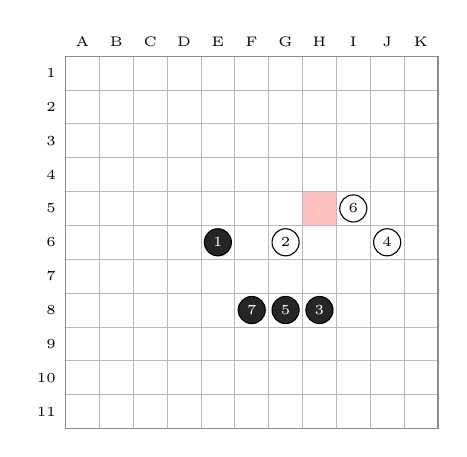
\begin{tikzpicture}[x=0.43cm, y=0.43cm]
\fill[red!25] (7,-4) rectangle (8,-5);
\draw[gray!55, line width=.3pt, step=1] (0,0) grid (11,-11);
\draw[gray!90] (0,0) rectangle (11,-11);
\node[font=\tiny, anchor=south] at (0.5,0) {A};
\node[font=\tiny, anchor=south] at (1.5,0) {B};
\node[font=\tiny, anchor=south] at (2.5,0) {C};
\node[font=\tiny, anchor=south] at (3.5,0) {D};
\node[font=\tiny, anchor=south] at (4.5,0) {E};
\node[font=\tiny, anchor=south] at (5.5,0) {F};
\node[font=\tiny, anchor=south] at (6.5,0) {G};
\node[font=\tiny, anchor=south] at (7.5,0) {H};
\node[font=\tiny, anchor=south] at (8.5,0) {I};
\node[font=\tiny, anchor=south] at (9.5,0) {J};
\node[font=\tiny, anchor=south] at (10.5,0) {K};
\node[font=\tiny, anchor=east] at (0,-0.5) {1};
\node[font=\tiny, anchor=east] at (0,-1.5) {2};
\node[font=\tiny, anchor=east] at (0,-2.5) {3};
\node[font=\tiny, anchor=east] at (0,-3.5) {4};
\node[font=\tiny, anchor=east] at (0,-4.5) {5};
\node[font=\tiny, anchor=east] at (0,-5.5) {6};
\node[font=\tiny, anchor=east] at (0,-6.5) {7};
\node[font=\tiny, anchor=east] at (0,-7.5) {8};
\node[font=\tiny, anchor=east] at (0,-8.5) {9};
\node[font=\tiny, anchor=east] at (0,-9.5) {10};
\node[font=\tiny, anchor=east] at (0,-10.5) {11};
\draw[fill=white, line width=.4pt] (8.5,-4.5) circle (.40);
\node[font=\tiny, text=black, inner sep=0pt] at (8.5,-4.5) {6};
\draw[fill=black!85, line width=.4pt] (4.5,-5.5) circle (.40);
\node[font=\tiny, text=white, inner sep=0pt] at (4.5,-5.5) {1};
\draw[fill=white, line width=.4pt] (6.5,-5.5) circle (.40);
\node[font=\tiny, text=black, inner sep=0pt] at (6.5,-5.5) {2};
\draw[fill=white, line width=.4pt] (9.5,-5.5) circle (.40);
\node[font=\tiny, text=black, inner sep=0pt] at (9.5,-5.5) {4};
\draw[fill=black!85, line width=.4pt] (5.5,-7.5) circle (.40);
\node[font=\tiny, text=white, inner sep=0pt] at (5.5,-7.5) {7};
\draw[fill=black!85, line width=.4pt] (6.5,-7.5) circle (.40);
\node[font=\tiny, text=white, inner sep=0pt] at (6.5,-7.5) {5};
\draw[fill=black!85, line width=.4pt] (7.5,-7.5) circle (.40);
\node[font=\tiny, text=white, inner sep=0pt] at (7.5,-7.5) {3};
\end{tikzpicture}
    \caption{Trước nước 8 (O đi; ô đỏ là nước đã chọn)}
  \end{subfigure}\hfill
  \begin{subfigure}[t]{.48\linewidth}
    \centering
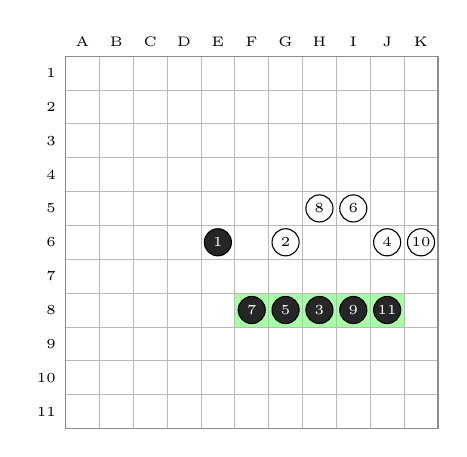
\begin{tikzpicture}[x=0.43cm, y=0.43cm]
\fill[green!35] (9,-7) rectangle (10,-8);
\fill[green!35] (8,-7) rectangle (9,-8);
\fill[green!35] (7,-7) rectangle (8,-8);
\fill[green!35] (6,-7) rectangle (7,-8);
\fill[green!35] (5,-7) rectangle (6,-8);
\draw[gray!55, line width=.3pt, step=1] (0,0) grid (11,-11);
\draw[gray!90] (0,0) rectangle (11,-11);
\node[font=\tiny, anchor=south] at (0.5,0) {A};
\node[font=\tiny, anchor=south] at (1.5,0) {B};
\node[font=\tiny, anchor=south] at (2.5,0) {C};
\node[font=\tiny, anchor=south] at (3.5,0) {D};
\node[font=\tiny, anchor=south] at (4.5,0) {E};
\node[font=\tiny, anchor=south] at (5.5,0) {F};
\node[font=\tiny, anchor=south] at (6.5,0) {G};
\node[font=\tiny, anchor=south] at (7.5,0) {H};
\node[font=\tiny, anchor=south] at (8.5,0) {I};
\node[font=\tiny, anchor=south] at (9.5,0) {J};
\node[font=\tiny, anchor=south] at (10.5,0) {K};
\node[font=\tiny, anchor=east] at (0,-0.5) {1};
\node[font=\tiny, anchor=east] at (0,-1.5) {2};
\node[font=\tiny, anchor=east] at (0,-2.5) {3};
\node[font=\tiny, anchor=east] at (0,-3.5) {4};
\node[font=\tiny, anchor=east] at (0,-4.5) {5};
\node[font=\tiny, anchor=east] at (0,-5.5) {6};
\node[font=\tiny, anchor=east] at (0,-6.5) {7};
\node[font=\tiny, anchor=east] at (0,-7.5) {8};
\node[font=\tiny, anchor=east] at (0,-8.5) {9};
\node[font=\tiny, anchor=east] at (0,-9.5) {10};
\node[font=\tiny, anchor=east] at (0,-10.5) {11};
\draw[fill=white, line width=.4pt] (7.5,-4.5) circle (.40);
\node[font=\tiny, text=black, inner sep=0pt] at (7.5,-4.5) {8};
\draw[fill=white, line width=.4pt] (8.5,-4.5) circle (.40);
\node[font=\tiny, text=black, inner sep=0pt] at (8.5,-4.5) {6};
\draw[fill=black!85, line width=.4pt] (4.5,-5.5) circle (.40);
\node[font=\tiny, text=white, inner sep=0pt] at (4.5,-5.5) {1};
\draw[fill=white, line width=.4pt] (6.5,-5.5) circle (.40);
\node[font=\tiny, text=black, inner sep=0pt] at (6.5,-5.5) {2};
\draw[fill=white, line width=.4pt] (9.5,-5.5) circle (.40);
\node[font=\tiny, text=black, inner sep=0pt] at (9.5,-5.5) {4};
\draw[fill=white, line width=.4pt] (10.5,-5.5) circle (.40);
\node[font=\tiny, text=black, inner sep=0pt] at (10.5,-5.5) {10};
\draw[fill=black!85, line width=.4pt] (5.5,-7.5) circle (.40);
\node[font=\tiny, text=white, inner sep=0pt] at (5.5,-7.5) {7};
\draw[fill=black!85, line width=.4pt] (6.5,-7.5) circle (.40);
\node[font=\tiny, text=white, inner sep=0pt] at (6.5,-7.5) {5};
\draw[fill=black!85, line width=.4pt] (7.5,-7.5) circle (.40);
\node[font=\tiny, text=white, inner sep=0pt] at (7.5,-7.5) {3};
\draw[fill=black!85, line width=.4pt] (8.5,-7.5) circle (.40);
\node[font=\tiny, text=white, inner sep=0pt] at (8.5,-7.5) {9};
\draw[fill=black!85, line width=.4pt] (9.5,-7.5) circle (.40);
\node[font=\tiny, text=white, inner sep=0pt] at (9.5,-7.5) {11};
\end{tikzpicture}
    \caption{Thế cuối (ô xanh: dãy thắng)}
  \end{subfigure}
  \caption{Ván 2143 (L8 cầm X, L4 cầm O).}
  \label{fig:cs-van-22}
\end{figure}
{\footnotesize\linespread{1}\selectfont
\noindent\begin{tabularx}{\linewidth}{*{6}{X}}
\toprule
1.~X E6$^\ast$ & 3.~X H8$^\ast$ & 5.~X G8 & 7.~X F8 & 9.~X I8 & 11.~X J8 \\
2.~O G6$^\ast$ & 4.~O J6 & 6.~O I5 & 8.~O H5 & 10.~O K6 &  \\
\bottomrule
\end{tabularx}\par}
\paragraph{Diễn biến chiến thuật.}
\begin{itemize}\small
\setlength{\itemsep}{0pt}
  \item Nước 8 (O=L4, H5): để đối thủ có VCF: E8--D8--I8.
  \item Nước 9 (X=L8, I8): đang có VCF 2 nước và đi đúng một đường (E8--D8--I8 là đường ngắn nhất).
  \item Nước 10 (O=L4, K6): đối thủ đang có các ô thắng E8, J8, không đỡ hết được.
  \item Nước 11 (X=L8, J8): thắng ngay.
\end{itemize}
Thời gian trung vị mỗi nước: X 76,1 ms, O 63,2 ms.
\clearpage

\subsection{L5 -- L6: ván 2208}
\label{sec:cs-van-23}
X: \texttt{L5-PolicySL}; O: \texttt{L6-PolicyRL}; khai cuộc 4 (4 nước, đánh dấu $\ast$); 29 nước; kết quả: X (L5) thắng. Cả cặp: L5 thắng 40, hoà 1, thua 59 trên 100 ván; trung vị 29 nước.
\begin{figure}[H]
  \centering
  \begin{subfigure}[t]{.48\linewidth}
    \centering
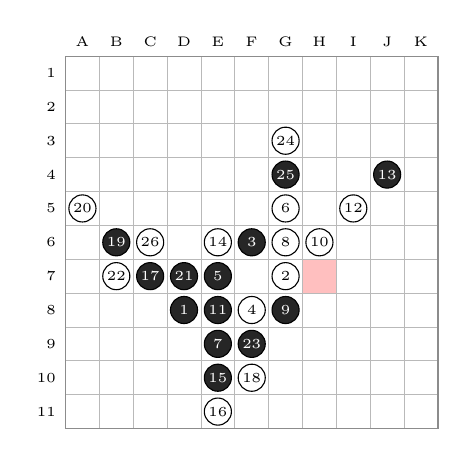
\begin{tikzpicture}[x=0.43cm, y=0.43cm]
\fill[red!25] (7,-6) rectangle (8,-7);
\draw[gray!55, line width=.3pt, step=1] (0,0) grid (11,-11);
\draw[gray!90] (0,0) rectangle (11,-11);
\node[font=\tiny, anchor=south] at (0.5,0) {A};
\node[font=\tiny, anchor=south] at (1.5,0) {B};
\node[font=\tiny, anchor=south] at (2.5,0) {C};
\node[font=\tiny, anchor=south] at (3.5,0) {D};
\node[font=\tiny, anchor=south] at (4.5,0) {E};
\node[font=\tiny, anchor=south] at (5.5,0) {F};
\node[font=\tiny, anchor=south] at (6.5,0) {G};
\node[font=\tiny, anchor=south] at (7.5,0) {H};
\node[font=\tiny, anchor=south] at (8.5,0) {I};
\node[font=\tiny, anchor=south] at (9.5,0) {J};
\node[font=\tiny, anchor=south] at (10.5,0) {K};
\node[font=\tiny, anchor=east] at (0,-0.5) {1};
\node[font=\tiny, anchor=east] at (0,-1.5) {2};
\node[font=\tiny, anchor=east] at (0,-2.5) {3};
\node[font=\tiny, anchor=east] at (0,-3.5) {4};
\node[font=\tiny, anchor=east] at (0,-4.5) {5};
\node[font=\tiny, anchor=east] at (0,-5.5) {6};
\node[font=\tiny, anchor=east] at (0,-6.5) {7};
\node[font=\tiny, anchor=east] at (0,-7.5) {8};
\node[font=\tiny, anchor=east] at (0,-8.5) {9};
\node[font=\tiny, anchor=east] at (0,-9.5) {10};
\node[font=\tiny, anchor=east] at (0,-10.5) {11};
\draw[fill=white, line width=.4pt] (6.5,-2.5) circle (.40);
\node[font=\tiny, text=black, inner sep=0pt] at (6.5,-2.5) {24};
\draw[fill=black!85, line width=.4pt] (6.5,-3.5) circle (.40);
\node[font=\tiny, text=white, inner sep=0pt] at (6.5,-3.5) {25};
\draw[fill=black!85, line width=.4pt] (9.5,-3.5) circle (.40);
\node[font=\tiny, text=white, inner sep=0pt] at (9.5,-3.5) {13};
\draw[fill=white, line width=.4pt] (0.5,-4.5) circle (.40);
\node[font=\tiny, text=black, inner sep=0pt] at (0.5,-4.5) {20};
\draw[fill=white, line width=.4pt] (6.5,-4.5) circle (.40);
\node[font=\tiny, text=black, inner sep=0pt] at (6.5,-4.5) {6};
\draw[fill=white, line width=.4pt] (8.5,-4.5) circle (.40);
\node[font=\tiny, text=black, inner sep=0pt] at (8.5,-4.5) {12};
\draw[fill=black!85, line width=.4pt] (1.5,-5.5) circle (.40);
\node[font=\tiny, text=white, inner sep=0pt] at (1.5,-5.5) {19};
\draw[fill=white, line width=.4pt] (2.5,-5.5) circle (.40);
\node[font=\tiny, text=black, inner sep=0pt] at (2.5,-5.5) {26};
\draw[fill=white, line width=.4pt] (4.5,-5.5) circle (.40);
\node[font=\tiny, text=black, inner sep=0pt] at (4.5,-5.5) {14};
\draw[fill=black!85, line width=.4pt] (5.5,-5.5) circle (.40);
\node[font=\tiny, text=white, inner sep=0pt] at (5.5,-5.5) {3};
\draw[fill=white, line width=.4pt] (6.5,-5.5) circle (.40);
\node[font=\tiny, text=black, inner sep=0pt] at (6.5,-5.5) {8};
\draw[fill=white, line width=.4pt] (7.5,-5.5) circle (.40);
\node[font=\tiny, text=black, inner sep=0pt] at (7.5,-5.5) {10};
\draw[fill=white, line width=.4pt] (1.5,-6.5) circle (.40);
\node[font=\tiny, text=black, inner sep=0pt] at (1.5,-6.5) {22};
\draw[fill=black!85, line width=.4pt] (2.5,-6.5) circle (.40);
\node[font=\tiny, text=white, inner sep=0pt] at (2.5,-6.5) {17};
\draw[fill=black!85, line width=.4pt] (3.5,-6.5) circle (.40);
\node[font=\tiny, text=white, inner sep=0pt] at (3.5,-6.5) {21};
\draw[fill=black!85, line width=.4pt] (4.5,-6.5) circle (.40);
\node[font=\tiny, text=white, inner sep=0pt] at (4.5,-6.5) {5};
\draw[fill=white, line width=.4pt] (6.5,-6.5) circle (.40);
\node[font=\tiny, text=black, inner sep=0pt] at (6.5,-6.5) {2};
\draw[fill=black!85, line width=.4pt] (3.5,-7.5) circle (.40);
\node[font=\tiny, text=white, inner sep=0pt] at (3.5,-7.5) {1};
\draw[fill=black!85, line width=.4pt] (4.5,-7.5) circle (.40);
\node[font=\tiny, text=white, inner sep=0pt] at (4.5,-7.5) {11};
\draw[fill=white, line width=.4pt] (5.5,-7.5) circle (.40);
\node[font=\tiny, text=black, inner sep=0pt] at (5.5,-7.5) {4};
\draw[fill=black!85, line width=.4pt] (6.5,-7.5) circle (.40);
\node[font=\tiny, text=white, inner sep=0pt] at (6.5,-7.5) {9};
\draw[fill=black!85, line width=.4pt] (4.5,-8.5) circle (.40);
\node[font=\tiny, text=white, inner sep=0pt] at (4.5,-8.5) {7};
\draw[fill=black!85, line width=.4pt] (5.5,-8.5) circle (.40);
\node[font=\tiny, text=white, inner sep=0pt] at (5.5,-8.5) {23};
\draw[fill=black!85, line width=.4pt] (4.5,-9.5) circle (.40);
\node[font=\tiny, text=white, inner sep=0pt] at (4.5,-9.5) {15};
\draw[fill=white, line width=.4pt] (5.5,-9.5) circle (.40);
\node[font=\tiny, text=black, inner sep=0pt] at (5.5,-9.5) {18};
\draw[fill=white, line width=.4pt] (4.5,-10.5) circle (.40);
\node[font=\tiny, text=black, inner sep=0pt] at (4.5,-10.5) {16};
\end{tikzpicture}
    \caption{Trước nước 27 (X đi; ô đỏ là nước đã chọn)}
  \end{subfigure}\hfill
  \begin{subfigure}[t]{.48\linewidth}
    \centering
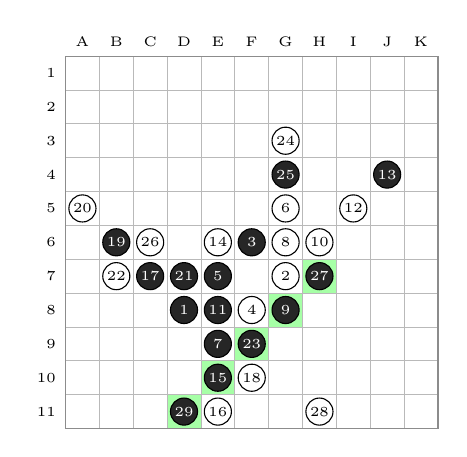
\begin{tikzpicture}[x=0.43cm, y=0.43cm]
\fill[green!35] (3,-10) rectangle (4,-11);
\fill[green!35] (4,-9) rectangle (5,-10);
\fill[green!35] (5,-8) rectangle (6,-9);
\fill[green!35] (6,-7) rectangle (7,-8);
\fill[green!35] (7,-6) rectangle (8,-7);
\draw[gray!55, line width=.3pt, step=1] (0,0) grid (11,-11);
\draw[gray!90] (0,0) rectangle (11,-11);
\node[font=\tiny, anchor=south] at (0.5,0) {A};
\node[font=\tiny, anchor=south] at (1.5,0) {B};
\node[font=\tiny, anchor=south] at (2.5,0) {C};
\node[font=\tiny, anchor=south] at (3.5,0) {D};
\node[font=\tiny, anchor=south] at (4.5,0) {E};
\node[font=\tiny, anchor=south] at (5.5,0) {F};
\node[font=\tiny, anchor=south] at (6.5,0) {G};
\node[font=\tiny, anchor=south] at (7.5,0) {H};
\node[font=\tiny, anchor=south] at (8.5,0) {I};
\node[font=\tiny, anchor=south] at (9.5,0) {J};
\node[font=\tiny, anchor=south] at (10.5,0) {K};
\node[font=\tiny, anchor=east] at (0,-0.5) {1};
\node[font=\tiny, anchor=east] at (0,-1.5) {2};
\node[font=\tiny, anchor=east] at (0,-2.5) {3};
\node[font=\tiny, anchor=east] at (0,-3.5) {4};
\node[font=\tiny, anchor=east] at (0,-4.5) {5};
\node[font=\tiny, anchor=east] at (0,-5.5) {6};
\node[font=\tiny, anchor=east] at (0,-6.5) {7};
\node[font=\tiny, anchor=east] at (0,-7.5) {8};
\node[font=\tiny, anchor=east] at (0,-8.5) {9};
\node[font=\tiny, anchor=east] at (0,-9.5) {10};
\node[font=\tiny, anchor=east] at (0,-10.5) {11};
\draw[fill=white, line width=.4pt] (6.5,-2.5) circle (.40);
\node[font=\tiny, text=black, inner sep=0pt] at (6.5,-2.5) {24};
\draw[fill=black!85, line width=.4pt] (6.5,-3.5) circle (.40);
\node[font=\tiny, text=white, inner sep=0pt] at (6.5,-3.5) {25};
\draw[fill=black!85, line width=.4pt] (9.5,-3.5) circle (.40);
\node[font=\tiny, text=white, inner sep=0pt] at (9.5,-3.5) {13};
\draw[fill=white, line width=.4pt] (0.5,-4.5) circle (.40);
\node[font=\tiny, text=black, inner sep=0pt] at (0.5,-4.5) {20};
\draw[fill=white, line width=.4pt] (6.5,-4.5) circle (.40);
\node[font=\tiny, text=black, inner sep=0pt] at (6.5,-4.5) {6};
\draw[fill=white, line width=.4pt] (8.5,-4.5) circle (.40);
\node[font=\tiny, text=black, inner sep=0pt] at (8.5,-4.5) {12};
\draw[fill=black!85, line width=.4pt] (1.5,-5.5) circle (.40);
\node[font=\tiny, text=white, inner sep=0pt] at (1.5,-5.5) {19};
\draw[fill=white, line width=.4pt] (2.5,-5.5) circle (.40);
\node[font=\tiny, text=black, inner sep=0pt] at (2.5,-5.5) {26};
\draw[fill=white, line width=.4pt] (4.5,-5.5) circle (.40);
\node[font=\tiny, text=black, inner sep=0pt] at (4.5,-5.5) {14};
\draw[fill=black!85, line width=.4pt] (5.5,-5.5) circle (.40);
\node[font=\tiny, text=white, inner sep=0pt] at (5.5,-5.5) {3};
\draw[fill=white, line width=.4pt] (6.5,-5.5) circle (.40);
\node[font=\tiny, text=black, inner sep=0pt] at (6.5,-5.5) {8};
\draw[fill=white, line width=.4pt] (7.5,-5.5) circle (.40);
\node[font=\tiny, text=black, inner sep=0pt] at (7.5,-5.5) {10};
\draw[fill=white, line width=.4pt] (1.5,-6.5) circle (.40);
\node[font=\tiny, text=black, inner sep=0pt] at (1.5,-6.5) {22};
\draw[fill=black!85, line width=.4pt] (2.5,-6.5) circle (.40);
\node[font=\tiny, text=white, inner sep=0pt] at (2.5,-6.5) {17};
\draw[fill=black!85, line width=.4pt] (3.5,-6.5) circle (.40);
\node[font=\tiny, text=white, inner sep=0pt] at (3.5,-6.5) {21};
\draw[fill=black!85, line width=.4pt] (4.5,-6.5) circle (.40);
\node[font=\tiny, text=white, inner sep=0pt] at (4.5,-6.5) {5};
\draw[fill=white, line width=.4pt] (6.5,-6.5) circle (.40);
\node[font=\tiny, text=black, inner sep=0pt] at (6.5,-6.5) {2};
\draw[fill=black!85, line width=.4pt] (7.5,-6.5) circle (.40);
\node[font=\tiny, text=white, inner sep=0pt] at (7.5,-6.5) {27};
\draw[fill=black!85, line width=.4pt] (3.5,-7.5) circle (.40);
\node[font=\tiny, text=white, inner sep=0pt] at (3.5,-7.5) {1};
\draw[fill=black!85, line width=.4pt] (4.5,-7.5) circle (.40);
\node[font=\tiny, text=white, inner sep=0pt] at (4.5,-7.5) {11};
\draw[fill=white, line width=.4pt] (5.5,-7.5) circle (.40);
\node[font=\tiny, text=black, inner sep=0pt] at (5.5,-7.5) {4};
\draw[fill=black!85, line width=.4pt] (6.5,-7.5) circle (.40);
\node[font=\tiny, text=white, inner sep=0pt] at (6.5,-7.5) {9};
\draw[fill=black!85, line width=.4pt] (4.5,-8.5) circle (.40);
\node[font=\tiny, text=white, inner sep=0pt] at (4.5,-8.5) {7};
\draw[fill=black!85, line width=.4pt] (5.5,-8.5) circle (.40);
\node[font=\tiny, text=white, inner sep=0pt] at (5.5,-8.5) {23};
\draw[fill=black!85, line width=.4pt] (4.5,-9.5) circle (.40);
\node[font=\tiny, text=white, inner sep=0pt] at (4.5,-9.5) {15};
\draw[fill=white, line width=.4pt] (5.5,-9.5) circle (.40);
\node[font=\tiny, text=black, inner sep=0pt] at (5.5,-9.5) {18};
\draw[fill=black!85, line width=.4pt] (3.5,-10.5) circle (.40);
\node[font=\tiny, text=white, inner sep=0pt] at (3.5,-10.5) {29};
\draw[fill=white, line width=.4pt] (4.5,-10.5) circle (.40);
\node[font=\tiny, text=black, inner sep=0pt] at (4.5,-10.5) {16};
\draw[fill=white, line width=.4pt] (7.5,-10.5) circle (.40);
\node[font=\tiny, text=black, inner sep=0pt] at (7.5,-10.5) {28};
\end{tikzpicture}
    \caption{Thế cuối (ô xanh: dãy thắng)}
  \end{subfigure}
  \caption{Ván 2208 (L5 cầm X, L6 cầm O).}
  \label{fig:cs-van-23}
\end{figure}
{\footnotesize\linespread{1}\selectfont
\noindent\begin{tabularx}{\linewidth}{*{6}{X}}
\toprule
1.~X D8$^\ast$ & 6.~O G5 & 11.~X E8 & 16.~O E11 & 21.~X D7 & 26.~O C6 \\
2.~O G7$^\ast$ & 7.~X E9 & 12.~O I5 & 17.~X C7 & 22.~O B7 & 27.~X H7 \\
3.~X F6$^\ast$ & 8.~O G6 & 13.~X J4 & 18.~O F10 & 23.~X F9 & 28.~O H11 \\
4.~O F8$^\ast$ & 9.~X G8 & 14.~O E6 & 19.~X B6 & 24.~O G3 & 29.~X D11 \\
5.~X E7 & 10.~O H6 & 15.~X E10 & 20.~O A5 & 25.~X G4 &  \\
\bottomrule
\end{tabularx}\par}
\paragraph{Diễn biến chiến thuật.}
\begin{itemize}\small
\setlength{\itemsep}{0pt}
  \item Nước 13 (X=L5, J4): chặn ô thắng J4.
  \item Nước 16 (O=L6, E11): chặn ô thắng E11.
  \item Nước 20 (O=L6, A5): chặn ô thắng A5.
  \item Nước 25 (X=L5, G4): chặn ô thắng G4.
  \item Nước 26 (O=L6, C6): không còn nước nào ngăn được VCF của đối thủ.
  \item Nước 27 (X=L5, H7): đang có VCF 2 nước và đi đúng một đường (H7--I6--D11 là đường ngắn nhất).
  \item Nước 28 (O=L6, H11): đối thủ đang có các ô thắng I6, D11, không đỡ hết được.
  \item Nước 29 (X=L5, D11): thắng ngay.
\end{itemize}
Thời gian trung vị mỗi nước: X 1,1 ms, O 1,1 ms.
\clearpage

\subsection{L5 -- L7: ván 2367}
\label{sec:cs-van-24}
X: \texttt{L7-PUCT}; O: \texttt{L5-PolicySL}; khai cuộc 33 (4 nước, đánh dấu $\ast$); 25 nước; kết quả: X (L7) thắng. Cả cặp: L5 thắng 6, hoà 1, thua 93 trên 100 ván; trung vị 25 nước.
\begin{figure}[H]
  \centering
  \begin{subfigure}[t]{.48\linewidth}
    \centering
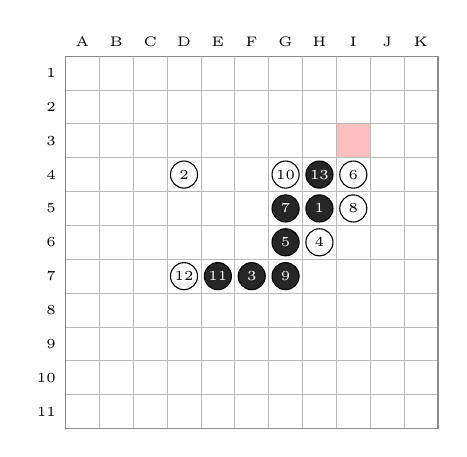
\begin{tikzpicture}[x=0.43cm, y=0.43cm]
\fill[red!25] (8,-2) rectangle (9,-3);
\draw[gray!55, line width=.3pt, step=1] (0,0) grid (11,-11);
\draw[gray!90] (0,0) rectangle (11,-11);
\node[font=\tiny, anchor=south] at (0.5,0) {A};
\node[font=\tiny, anchor=south] at (1.5,0) {B};
\node[font=\tiny, anchor=south] at (2.5,0) {C};
\node[font=\tiny, anchor=south] at (3.5,0) {D};
\node[font=\tiny, anchor=south] at (4.5,0) {E};
\node[font=\tiny, anchor=south] at (5.5,0) {F};
\node[font=\tiny, anchor=south] at (6.5,0) {G};
\node[font=\tiny, anchor=south] at (7.5,0) {H};
\node[font=\tiny, anchor=south] at (8.5,0) {I};
\node[font=\tiny, anchor=south] at (9.5,0) {J};
\node[font=\tiny, anchor=south] at (10.5,0) {K};
\node[font=\tiny, anchor=east] at (0,-0.5) {1};
\node[font=\tiny, anchor=east] at (0,-1.5) {2};
\node[font=\tiny, anchor=east] at (0,-2.5) {3};
\node[font=\tiny, anchor=east] at (0,-3.5) {4};
\node[font=\tiny, anchor=east] at (0,-4.5) {5};
\node[font=\tiny, anchor=east] at (0,-5.5) {6};
\node[font=\tiny, anchor=east] at (0,-6.5) {7};
\node[font=\tiny, anchor=east] at (0,-7.5) {8};
\node[font=\tiny, anchor=east] at (0,-8.5) {9};
\node[font=\tiny, anchor=east] at (0,-9.5) {10};
\node[font=\tiny, anchor=east] at (0,-10.5) {11};
\draw[fill=white, line width=.4pt] (3.5,-3.5) circle (.40);
\node[font=\tiny, text=black, inner sep=0pt] at (3.5,-3.5) {2};
\draw[fill=white, line width=.4pt] (6.5,-3.5) circle (.40);
\node[font=\tiny, text=black, inner sep=0pt] at (6.5,-3.5) {10};
\draw[fill=black!85, line width=.4pt] (7.5,-3.5) circle (.40);
\node[font=\tiny, text=white, inner sep=0pt] at (7.5,-3.5) {13};
\draw[fill=white, line width=.4pt] (8.5,-3.5) circle (.40);
\node[font=\tiny, text=black, inner sep=0pt] at (8.5,-3.5) {6};
\draw[fill=black!85, line width=.4pt] (6.5,-4.5) circle (.40);
\node[font=\tiny, text=white, inner sep=0pt] at (6.5,-4.5) {7};
\draw[fill=black!85, line width=.4pt] (7.5,-4.5) circle (.40);
\node[font=\tiny, text=white, inner sep=0pt] at (7.5,-4.5) {1};
\draw[fill=white, line width=.4pt] (8.5,-4.5) circle (.40);
\node[font=\tiny, text=black, inner sep=0pt] at (8.5,-4.5) {8};
\draw[fill=black!85, line width=.4pt] (6.5,-5.5) circle (.40);
\node[font=\tiny, text=white, inner sep=0pt] at (6.5,-5.5) {5};
\draw[fill=white, line width=.4pt] (7.5,-5.5) circle (.40);
\node[font=\tiny, text=black, inner sep=0pt] at (7.5,-5.5) {4};
\draw[fill=white, line width=.4pt] (3.5,-6.5) circle (.40);
\node[font=\tiny, text=black, inner sep=0pt] at (3.5,-6.5) {12};
\draw[fill=black!85, line width=.4pt] (4.5,-6.5) circle (.40);
\node[font=\tiny, text=white, inner sep=0pt] at (4.5,-6.5) {11};
\draw[fill=black!85, line width=.4pt] (5.5,-6.5) circle (.40);
\node[font=\tiny, text=white, inner sep=0pt] at (5.5,-6.5) {3};
\draw[fill=black!85, line width=.4pt] (6.5,-6.5) circle (.40);
\node[font=\tiny, text=white, inner sep=0pt] at (6.5,-6.5) {9};
\end{tikzpicture}
    \caption{Trước nước 14 (O đi; ô đỏ là nước đã chọn)}
  \end{subfigure}\hfill
  \begin{subfigure}[t]{.48\linewidth}
    \centering
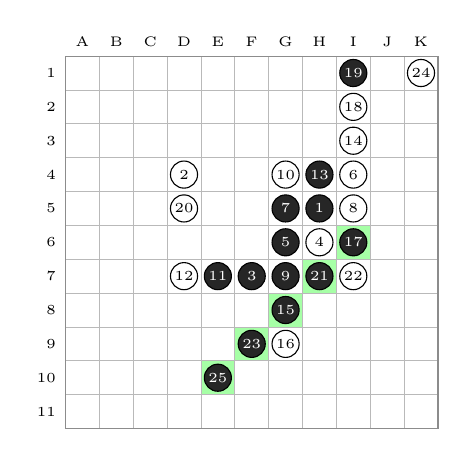
\begin{tikzpicture}[x=0.43cm, y=0.43cm]
\fill[green!35] (4,-9) rectangle (5,-10);
\fill[green!35] (5,-8) rectangle (6,-9);
\fill[green!35] (6,-7) rectangle (7,-8);
\fill[green!35] (7,-6) rectangle (8,-7);
\fill[green!35] (8,-5) rectangle (9,-6);
\draw[gray!55, line width=.3pt, step=1] (0,0) grid (11,-11);
\draw[gray!90] (0,0) rectangle (11,-11);
\node[font=\tiny, anchor=south] at (0.5,0) {A};
\node[font=\tiny, anchor=south] at (1.5,0) {B};
\node[font=\tiny, anchor=south] at (2.5,0) {C};
\node[font=\tiny, anchor=south] at (3.5,0) {D};
\node[font=\tiny, anchor=south] at (4.5,0) {E};
\node[font=\tiny, anchor=south] at (5.5,0) {F};
\node[font=\tiny, anchor=south] at (6.5,0) {G};
\node[font=\tiny, anchor=south] at (7.5,0) {H};
\node[font=\tiny, anchor=south] at (8.5,0) {I};
\node[font=\tiny, anchor=south] at (9.5,0) {J};
\node[font=\tiny, anchor=south] at (10.5,0) {K};
\node[font=\tiny, anchor=east] at (0,-0.5) {1};
\node[font=\tiny, anchor=east] at (0,-1.5) {2};
\node[font=\tiny, anchor=east] at (0,-2.5) {3};
\node[font=\tiny, anchor=east] at (0,-3.5) {4};
\node[font=\tiny, anchor=east] at (0,-4.5) {5};
\node[font=\tiny, anchor=east] at (0,-5.5) {6};
\node[font=\tiny, anchor=east] at (0,-6.5) {7};
\node[font=\tiny, anchor=east] at (0,-7.5) {8};
\node[font=\tiny, anchor=east] at (0,-8.5) {9};
\node[font=\tiny, anchor=east] at (0,-9.5) {10};
\node[font=\tiny, anchor=east] at (0,-10.5) {11};
\draw[fill=black!85, line width=.4pt] (8.5,-0.5) circle (.40);
\node[font=\tiny, text=white, inner sep=0pt] at (8.5,-0.5) {19};
\draw[fill=white, line width=.4pt] (10.5,-0.5) circle (.40);
\node[font=\tiny, text=black, inner sep=0pt] at (10.5,-0.5) {24};
\draw[fill=white, line width=.4pt] (8.5,-1.5) circle (.40);
\node[font=\tiny, text=black, inner sep=0pt] at (8.5,-1.5) {18};
\draw[fill=white, line width=.4pt] (8.5,-2.5) circle (.40);
\node[font=\tiny, text=black, inner sep=0pt] at (8.5,-2.5) {14};
\draw[fill=white, line width=.4pt] (3.5,-3.5) circle (.40);
\node[font=\tiny, text=black, inner sep=0pt] at (3.5,-3.5) {2};
\draw[fill=white, line width=.4pt] (6.5,-3.5) circle (.40);
\node[font=\tiny, text=black, inner sep=0pt] at (6.5,-3.5) {10};
\draw[fill=black!85, line width=.4pt] (7.5,-3.5) circle (.40);
\node[font=\tiny, text=white, inner sep=0pt] at (7.5,-3.5) {13};
\draw[fill=white, line width=.4pt] (8.5,-3.5) circle (.40);
\node[font=\tiny, text=black, inner sep=0pt] at (8.5,-3.5) {6};
\draw[fill=white, line width=.4pt] (3.5,-4.5) circle (.40);
\node[font=\tiny, text=black, inner sep=0pt] at (3.5,-4.5) {20};
\draw[fill=black!85, line width=.4pt] (6.5,-4.5) circle (.40);
\node[font=\tiny, text=white, inner sep=0pt] at (6.5,-4.5) {7};
\draw[fill=black!85, line width=.4pt] (7.5,-4.5) circle (.40);
\node[font=\tiny, text=white, inner sep=0pt] at (7.5,-4.5) {1};
\draw[fill=white, line width=.4pt] (8.5,-4.5) circle (.40);
\node[font=\tiny, text=black, inner sep=0pt] at (8.5,-4.5) {8};
\draw[fill=black!85, line width=.4pt] (6.5,-5.5) circle (.40);
\node[font=\tiny, text=white, inner sep=0pt] at (6.5,-5.5) {5};
\draw[fill=white, line width=.4pt] (7.5,-5.5) circle (.40);
\node[font=\tiny, text=black, inner sep=0pt] at (7.5,-5.5) {4};
\draw[fill=black!85, line width=.4pt] (8.5,-5.5) circle (.40);
\node[font=\tiny, text=white, inner sep=0pt] at (8.5,-5.5) {17};
\draw[fill=white, line width=.4pt] (3.5,-6.5) circle (.40);
\node[font=\tiny, text=black, inner sep=0pt] at (3.5,-6.5) {12};
\draw[fill=black!85, line width=.4pt] (4.5,-6.5) circle (.40);
\node[font=\tiny, text=white, inner sep=0pt] at (4.5,-6.5) {11};
\draw[fill=black!85, line width=.4pt] (5.5,-6.5) circle (.40);
\node[font=\tiny, text=white, inner sep=0pt] at (5.5,-6.5) {3};
\draw[fill=black!85, line width=.4pt] (6.5,-6.5) circle (.40);
\node[font=\tiny, text=white, inner sep=0pt] at (6.5,-6.5) {9};
\draw[fill=black!85, line width=.4pt] (7.5,-6.5) circle (.40);
\node[font=\tiny, text=white, inner sep=0pt] at (7.5,-6.5) {21};
\draw[fill=white, line width=.4pt] (8.5,-6.5) circle (.40);
\node[font=\tiny, text=black, inner sep=0pt] at (8.5,-6.5) {22};
\draw[fill=black!85, line width=.4pt] (6.5,-7.5) circle (.40);
\node[font=\tiny, text=white, inner sep=0pt] at (6.5,-7.5) {15};
\draw[fill=black!85, line width=.4pt] (5.5,-8.5) circle (.40);
\node[font=\tiny, text=white, inner sep=0pt] at (5.5,-8.5) {23};
\draw[fill=white, line width=.4pt] (6.5,-8.5) circle (.40);
\node[font=\tiny, text=black, inner sep=0pt] at (6.5,-8.5) {16};
\draw[fill=black!85, line width=.4pt] (4.5,-9.5) circle (.40);
\node[font=\tiny, text=white, inner sep=0pt] at (4.5,-9.5) {25};
\end{tikzpicture}
    \caption{Thế cuối (ô xanh: dãy thắng)}
  \end{subfigure}
  \caption{Ván 2367 (L7 cầm X, L5 cầm O).}
  \label{fig:cs-van-24}
\end{figure}
{\footnotesize\linespread{1}\selectfont
\noindent\begin{tabularx}{\linewidth}{*{6}{X}}
\toprule
1.~X H5$^\ast$ & 6.~O I4 & 11.~X E7 & 16.~O G9 & 21.~X H7 &  \\
2.~O D4$^\ast$ & 7.~X G5 & 12.~O D7 & 17.~X I6 & 22.~O I7 &  \\
3.~X F7$^\ast$ & 8.~O I5 & 13.~X H4 & 18.~O I2 & 23.~X F9 &  \\
4.~O H6$^\ast$ & 9.~X G7 & 14.~O I3 & 19.~X I1 & 24.~O K1 &  \\
5.~X G6 & 10.~O G4 & 15.~X G8 & 20.~O D5 & 25.~X E10 &  \\
\bottomrule
\end{tabularx}\par}
\paragraph{Diễn biến chiến thuật.}
\begin{itemize}\small
\setlength{\itemsep}{0pt}
  \item Nước 14 (O=L5, I3): để đối thủ có VCF: D8--F6--E8--D9--G8--G9--F8--C8--H8.
  \item Nước 15 (X=L7, G8): đang có VCF 5 nước và đi đúng một đường (D8--F6--E8--D9--G8--G9--F8--C8--H8 là đường ngắn nhất).
  \item Nước 16 (O=L5, G9): chặn ô thắng G9.
  \item Nước 17 (X=L7, I6): bỏ lỡ VCF 4 nước: D8--F6--E8--D9--F8--C8--H8.
  \item Nước 19 (X=L7, I1): chặn ô thắng I1.
  \item Nước 20 (O=L5, D5): không còn nước nào ngăn được VCF của đối thủ.
  \item Nước 21 (X=L7, H7): đang có VCF 3 nước và đi đúng một đường (H7--I7--J5--K4--F9 là đường ngắn nhất).
  \item Nước 22 (O=L5, I7): chặn ô thắng I7.
  \item Nước 23 (X=L7, F9): đang có VCF 2 nước và đi đúng một đường (J5--K4--F9 là đường ngắn nhất).
  \item Nước 24 (O=L5, K1): đối thủ đang có các ô thắng J5, E10, không đỡ hết được.
  \item Nước 25 (X=L7, E10): thắng ngay.
\end{itemize}
Thời gian trung vị mỗi nước: X 91,2 ms, O 1,3 ms.
\clearpage

\subsection{L5 -- L8: ván 2467}
\label{sec:cs-van-25}
X: \texttt{L8-AlphaZero}; O: \texttt{L5-PolicySL}; khai cuộc 33 (4 nước, đánh dấu $\ast$); 25 nước; kết quả: X (L8) thắng. Cả cặp: L5 thắng 5, hoà 3, thua 92 trên 100 ván; trung vị 26 nước.
\begin{figure}[H]
  \centering
  \begin{subfigure}[t]{.48\linewidth}
    \centering
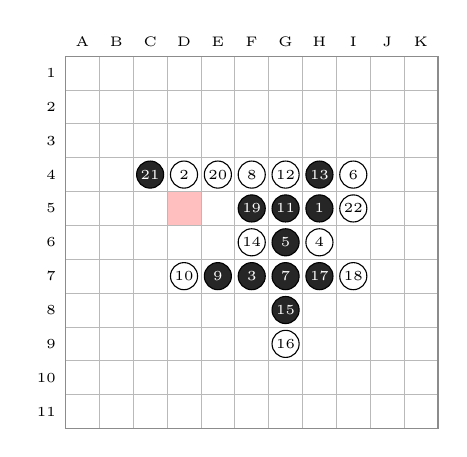
\begin{tikzpicture}[x=0.43cm, y=0.43cm]
\fill[red!25] (3,-4) rectangle (4,-5);
\draw[gray!55, line width=.3pt, step=1] (0,0) grid (11,-11);
\draw[gray!90] (0,0) rectangle (11,-11);
\node[font=\tiny, anchor=south] at (0.5,0) {A};
\node[font=\tiny, anchor=south] at (1.5,0) {B};
\node[font=\tiny, anchor=south] at (2.5,0) {C};
\node[font=\tiny, anchor=south] at (3.5,0) {D};
\node[font=\tiny, anchor=south] at (4.5,0) {E};
\node[font=\tiny, anchor=south] at (5.5,0) {F};
\node[font=\tiny, anchor=south] at (6.5,0) {G};
\node[font=\tiny, anchor=south] at (7.5,0) {H};
\node[font=\tiny, anchor=south] at (8.5,0) {I};
\node[font=\tiny, anchor=south] at (9.5,0) {J};
\node[font=\tiny, anchor=south] at (10.5,0) {K};
\node[font=\tiny, anchor=east] at (0,-0.5) {1};
\node[font=\tiny, anchor=east] at (0,-1.5) {2};
\node[font=\tiny, anchor=east] at (0,-2.5) {3};
\node[font=\tiny, anchor=east] at (0,-3.5) {4};
\node[font=\tiny, anchor=east] at (0,-4.5) {5};
\node[font=\tiny, anchor=east] at (0,-5.5) {6};
\node[font=\tiny, anchor=east] at (0,-6.5) {7};
\node[font=\tiny, anchor=east] at (0,-7.5) {8};
\node[font=\tiny, anchor=east] at (0,-8.5) {9};
\node[font=\tiny, anchor=east] at (0,-9.5) {10};
\node[font=\tiny, anchor=east] at (0,-10.5) {11};
\draw[fill=black!85, line width=.4pt] (2.5,-3.5) circle (.40);
\node[font=\tiny, text=white, inner sep=0pt] at (2.5,-3.5) {21};
\draw[fill=white, line width=.4pt] (3.5,-3.5) circle (.40);
\node[font=\tiny, text=black, inner sep=0pt] at (3.5,-3.5) {2};
\draw[fill=white, line width=.4pt] (4.5,-3.5) circle (.40);
\node[font=\tiny, text=black, inner sep=0pt] at (4.5,-3.5) {20};
\draw[fill=white, line width=.4pt] (5.5,-3.5) circle (.40);
\node[font=\tiny, text=black, inner sep=0pt] at (5.5,-3.5) {8};
\draw[fill=white, line width=.4pt] (6.5,-3.5) circle (.40);
\node[font=\tiny, text=black, inner sep=0pt] at (6.5,-3.5) {12};
\draw[fill=black!85, line width=.4pt] (7.5,-3.5) circle (.40);
\node[font=\tiny, text=white, inner sep=0pt] at (7.5,-3.5) {13};
\draw[fill=white, line width=.4pt] (8.5,-3.5) circle (.40);
\node[font=\tiny, text=black, inner sep=0pt] at (8.5,-3.5) {6};
\draw[fill=black!85, line width=.4pt] (5.5,-4.5) circle (.40);
\node[font=\tiny, text=white, inner sep=0pt] at (5.5,-4.5) {19};
\draw[fill=black!85, line width=.4pt] (6.5,-4.5) circle (.40);
\node[font=\tiny, text=white, inner sep=0pt] at (6.5,-4.5) {11};
\draw[fill=black!85, line width=.4pt] (7.5,-4.5) circle (.40);
\node[font=\tiny, text=white, inner sep=0pt] at (7.5,-4.5) {1};
\draw[fill=white, line width=.4pt] (8.5,-4.5) circle (.40);
\node[font=\tiny, text=black, inner sep=0pt] at (8.5,-4.5) {22};
\draw[fill=white, line width=.4pt] (5.5,-5.5) circle (.40);
\node[font=\tiny, text=black, inner sep=0pt] at (5.5,-5.5) {14};
\draw[fill=black!85, line width=.4pt] (6.5,-5.5) circle (.40);
\node[font=\tiny, text=white, inner sep=0pt] at (6.5,-5.5) {5};
\draw[fill=white, line width=.4pt] (7.5,-5.5) circle (.40);
\node[font=\tiny, text=black, inner sep=0pt] at (7.5,-5.5) {4};
\draw[fill=white, line width=.4pt] (3.5,-6.5) circle (.40);
\node[font=\tiny, text=black, inner sep=0pt] at (3.5,-6.5) {10};
\draw[fill=black!85, line width=.4pt] (4.5,-6.5) circle (.40);
\node[font=\tiny, text=white, inner sep=0pt] at (4.5,-6.5) {9};
\draw[fill=black!85, line width=.4pt] (5.5,-6.5) circle (.40);
\node[font=\tiny, text=white, inner sep=0pt] at (5.5,-6.5) {3};
\draw[fill=black!85, line width=.4pt] (6.5,-6.5) circle (.40);
\node[font=\tiny, text=white, inner sep=0pt] at (6.5,-6.5) {7};
\draw[fill=black!85, line width=.4pt] (7.5,-6.5) circle (.40);
\node[font=\tiny, text=white, inner sep=0pt] at (7.5,-6.5) {17};
\draw[fill=white, line width=.4pt] (8.5,-6.5) circle (.40);
\node[font=\tiny, text=black, inner sep=0pt] at (8.5,-6.5) {18};
\draw[fill=black!85, line width=.4pt] (6.5,-7.5) circle (.40);
\node[font=\tiny, text=white, inner sep=0pt] at (6.5,-7.5) {15};
\draw[fill=white, line width=.4pt] (6.5,-8.5) circle (.40);
\node[font=\tiny, text=black, inner sep=0pt] at (6.5,-8.5) {16};
\end{tikzpicture}
    \caption{Trước nước 23 (X đi; ô đỏ là nước đã chọn)}
  \end{subfigure}\hfill
  \begin{subfigure}[t]{.48\linewidth}
    \centering
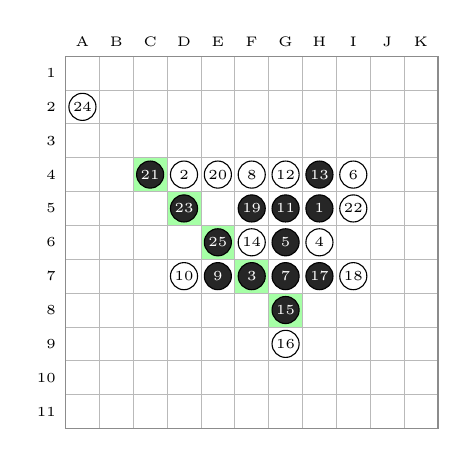
\begin{tikzpicture}[x=0.43cm, y=0.43cm]
\fill[green!35] (4,-5) rectangle (5,-6);
\fill[green!35] (5,-6) rectangle (6,-7);
\fill[green!35] (6,-7) rectangle (7,-8);
\fill[green!35] (3,-4) rectangle (4,-5);
\fill[green!35] (2,-3) rectangle (3,-4);
\draw[gray!55, line width=.3pt, step=1] (0,0) grid (11,-11);
\draw[gray!90] (0,0) rectangle (11,-11);
\node[font=\tiny, anchor=south] at (0.5,0) {A};
\node[font=\tiny, anchor=south] at (1.5,0) {B};
\node[font=\tiny, anchor=south] at (2.5,0) {C};
\node[font=\tiny, anchor=south] at (3.5,0) {D};
\node[font=\tiny, anchor=south] at (4.5,0) {E};
\node[font=\tiny, anchor=south] at (5.5,0) {F};
\node[font=\tiny, anchor=south] at (6.5,0) {G};
\node[font=\tiny, anchor=south] at (7.5,0) {H};
\node[font=\tiny, anchor=south] at (8.5,0) {I};
\node[font=\tiny, anchor=south] at (9.5,0) {J};
\node[font=\tiny, anchor=south] at (10.5,0) {K};
\node[font=\tiny, anchor=east] at (0,-0.5) {1};
\node[font=\tiny, anchor=east] at (0,-1.5) {2};
\node[font=\tiny, anchor=east] at (0,-2.5) {3};
\node[font=\tiny, anchor=east] at (0,-3.5) {4};
\node[font=\tiny, anchor=east] at (0,-4.5) {5};
\node[font=\tiny, anchor=east] at (0,-5.5) {6};
\node[font=\tiny, anchor=east] at (0,-6.5) {7};
\node[font=\tiny, anchor=east] at (0,-7.5) {8};
\node[font=\tiny, anchor=east] at (0,-8.5) {9};
\node[font=\tiny, anchor=east] at (0,-9.5) {10};
\node[font=\tiny, anchor=east] at (0,-10.5) {11};
\draw[fill=white, line width=.4pt] (0.5,-1.5) circle (.40);
\node[font=\tiny, text=black, inner sep=0pt] at (0.5,-1.5) {24};
\draw[fill=black!85, line width=.4pt] (2.5,-3.5) circle (.40);
\node[font=\tiny, text=white, inner sep=0pt] at (2.5,-3.5) {21};
\draw[fill=white, line width=.4pt] (3.5,-3.5) circle (.40);
\node[font=\tiny, text=black, inner sep=0pt] at (3.5,-3.5) {2};
\draw[fill=white, line width=.4pt] (4.5,-3.5) circle (.40);
\node[font=\tiny, text=black, inner sep=0pt] at (4.5,-3.5) {20};
\draw[fill=white, line width=.4pt] (5.5,-3.5) circle (.40);
\node[font=\tiny, text=black, inner sep=0pt] at (5.5,-3.5) {8};
\draw[fill=white, line width=.4pt] (6.5,-3.5) circle (.40);
\node[font=\tiny, text=black, inner sep=0pt] at (6.5,-3.5) {12};
\draw[fill=black!85, line width=.4pt] (7.5,-3.5) circle (.40);
\node[font=\tiny, text=white, inner sep=0pt] at (7.5,-3.5) {13};
\draw[fill=white, line width=.4pt] (8.5,-3.5) circle (.40);
\node[font=\tiny, text=black, inner sep=0pt] at (8.5,-3.5) {6};
\draw[fill=black!85, line width=.4pt] (3.5,-4.5) circle (.40);
\node[font=\tiny, text=white, inner sep=0pt] at (3.5,-4.5) {23};
\draw[fill=black!85, line width=.4pt] (5.5,-4.5) circle (.40);
\node[font=\tiny, text=white, inner sep=0pt] at (5.5,-4.5) {19};
\draw[fill=black!85, line width=.4pt] (6.5,-4.5) circle (.40);
\node[font=\tiny, text=white, inner sep=0pt] at (6.5,-4.5) {11};
\draw[fill=black!85, line width=.4pt] (7.5,-4.5) circle (.40);
\node[font=\tiny, text=white, inner sep=0pt] at (7.5,-4.5) {1};
\draw[fill=white, line width=.4pt] (8.5,-4.5) circle (.40);
\node[font=\tiny, text=black, inner sep=0pt] at (8.5,-4.5) {22};
\draw[fill=black!85, line width=.4pt] (4.5,-5.5) circle (.40);
\node[font=\tiny, text=white, inner sep=0pt] at (4.5,-5.5) {25};
\draw[fill=white, line width=.4pt] (5.5,-5.5) circle (.40);
\node[font=\tiny, text=black, inner sep=0pt] at (5.5,-5.5) {14};
\draw[fill=black!85, line width=.4pt] (6.5,-5.5) circle (.40);
\node[font=\tiny, text=white, inner sep=0pt] at (6.5,-5.5) {5};
\draw[fill=white, line width=.4pt] (7.5,-5.5) circle (.40);
\node[font=\tiny, text=black, inner sep=0pt] at (7.5,-5.5) {4};
\draw[fill=white, line width=.4pt] (3.5,-6.5) circle (.40);
\node[font=\tiny, text=black, inner sep=0pt] at (3.5,-6.5) {10};
\draw[fill=black!85, line width=.4pt] (4.5,-6.5) circle (.40);
\node[font=\tiny, text=white, inner sep=0pt] at (4.5,-6.5) {9};
\draw[fill=black!85, line width=.4pt] (5.5,-6.5) circle (.40);
\node[font=\tiny, text=white, inner sep=0pt] at (5.5,-6.5) {3};
\draw[fill=black!85, line width=.4pt] (6.5,-6.5) circle (.40);
\node[font=\tiny, text=white, inner sep=0pt] at (6.5,-6.5) {7};
\draw[fill=black!85, line width=.4pt] (7.5,-6.5) circle (.40);
\node[font=\tiny, text=white, inner sep=0pt] at (7.5,-6.5) {17};
\draw[fill=white, line width=.4pt] (8.5,-6.5) circle (.40);
\node[font=\tiny, text=black, inner sep=0pt] at (8.5,-6.5) {18};
\draw[fill=black!85, line width=.4pt] (6.5,-7.5) circle (.40);
\node[font=\tiny, text=white, inner sep=0pt] at (6.5,-7.5) {15};
\draw[fill=white, line width=.4pt] (6.5,-8.5) circle (.40);
\node[font=\tiny, text=black, inner sep=0pt] at (6.5,-8.5) {16};
\end{tikzpicture}
    \caption{Thế cuối (ô xanh: dãy thắng)}
  \end{subfigure}
  \caption{Ván 2467 (L8 cầm X, L5 cầm O).}
  \label{fig:cs-van-25}
\end{figure}
{\footnotesize\linespread{1}\selectfont
\noindent\begin{tabularx}{\linewidth}{*{6}{X}}
\toprule
1.~X H5$^\ast$ & 6.~O I4 & 11.~X G5 & 16.~O G9 & 21.~X C4 &  \\
2.~O D4$^\ast$ & 7.~X G7 & 12.~O G4 & 17.~X H7 & 22.~O I5 &  \\
3.~X F7$^\ast$ & 8.~O F4 & 13.~X H4 & 18.~O I7 & 23.~X D5 &  \\
4.~O H6$^\ast$ & 9.~X E7 & 14.~O F6 & 19.~X F5 & 24.~O A2 &  \\
5.~X G6 & 10.~O D7 & 15.~X G8 & 20.~O E4 & 25.~X E6 &  \\
\bottomrule
\end{tabularx}\par}
\paragraph{Diễn biến chiến thuật.}
\begin{itemize}\small
\setlength{\itemsep}{0pt}
  \item Nước 16 (O=L5, G9): chặn ô thắng G9.
  \item Nước 18 (O=L5, I7): chặn ô thắng I7.
  \item Nước 21 (X=L8, C4): chặn ô thắng C4.
  \item Nước 22 (O=L5, I5): không còn nước nào ngăn được VCF của đối thủ.
  \item Nước 23 (X=L8, D5): đang có VCF 2 nước và đi đúng một đường (D5--E5--E6 là đường ngắn nhất).
  \item Nước 24 (O=L5, A2): đối thủ đang có các ô thắng E5, E6, không đỡ hết được.
  \item Nước 25 (X=L8, E6): thắng ngay.
\end{itemize}
Thời gian trung vị mỗi nước: X 91,4 ms, O 1,3 ms.
\clearpage

\subsection{L6 -- L7: ván 2585}
\label{sec:cs-van-26}
X: \texttt{L7-PUCT}; O: \texttt{L6-PolicyRL}; khai cuộc 42 (4 nước, đánh dấu $\ast$); 25 nước; kết quả: X (L7) thắng. Cả cặp: L6 thắng 22, hoà 7, thua 71 trên 100 ván; trung vị 26 nước.
\begin{figure}[H]
  \centering
  \begin{subfigure}[t]{.48\linewidth}
    \centering
\begin{tikzpicture}[x=0.43cm, y=0.43cm]
\fill[red!25] (7,-8) rectangle (8,-9);
\draw[gray!55, line width=.3pt, step=1] (0,0) grid (11,-11);
\draw[gray!90] (0,0) rectangle (11,-11);
\node[font=\tiny, anchor=south] at (0.5,0) {A};
\node[font=\tiny, anchor=south] at (1.5,0) {B};
\node[font=\tiny, anchor=south] at (2.5,0) {C};
\node[font=\tiny, anchor=south] at (3.5,0) {D};
\node[font=\tiny, anchor=south] at (4.5,0) {E};
\node[font=\tiny, anchor=south] at (5.5,0) {F};
\node[font=\tiny, anchor=south] at (6.5,0) {G};
\node[font=\tiny, anchor=south] at (7.5,0) {H};
\node[font=\tiny, anchor=south] at (8.5,0) {I};
\node[font=\tiny, anchor=south] at (9.5,0) {J};
\node[font=\tiny, anchor=south] at (10.5,0) {K};
\node[font=\tiny, anchor=east] at (0,-0.5) {1};
\node[font=\tiny, anchor=east] at (0,-1.5) {2};
\node[font=\tiny, anchor=east] at (0,-2.5) {3};
\node[font=\tiny, anchor=east] at (0,-3.5) {4};
\node[font=\tiny, anchor=east] at (0,-4.5) {5};
\node[font=\tiny, anchor=east] at (0,-5.5) {6};
\node[font=\tiny, anchor=east] at (0,-6.5) {7};
\node[font=\tiny, anchor=east] at (0,-7.5) {8};
\node[font=\tiny, anchor=east] at (0,-8.5) {9};
\node[font=\tiny, anchor=east] at (0,-9.5) {10};
\node[font=\tiny, anchor=east] at (0,-10.5) {11};
\draw[fill=white, line width=.4pt] (4.5,-3.5) circle (.40);
\node[font=\tiny, text=black, inner sep=0pt] at (4.5,-3.5) {8};
\draw[fill=white, line width=.4pt] (5.5,-3.5) circle (.40);
\node[font=\tiny, text=black, inner sep=0pt] at (5.5,-3.5) {4};
\draw[fill=white, line width=.4pt] (3.5,-4.5) circle (.40);
\node[font=\tiny, text=black, inner sep=0pt] at (3.5,-4.5) {6};
\draw[fill=black!85, line width=.4pt] (4.5,-5.5) circle (.40);
\node[font=\tiny, text=white, inner sep=0pt] at (4.5,-5.5) {5};
\draw[fill=white, line width=.4pt] (5.5,-5.5) circle (.40);
\node[font=\tiny, text=black, inner sep=0pt] at (5.5,-5.5) {10};
\draw[fill=white, line width=.4pt] (6.5,-5.5) circle (.40);
\node[font=\tiny, text=black, inner sep=0pt] at (6.5,-5.5) {2};
\draw[fill=white, line width=.4pt] (8.5,-5.5) circle (.40);
\node[font=\tiny, text=black, inner sep=0pt] at (8.5,-5.5) {14};
\draw[fill=black!85, line width=.4pt] (5.5,-6.5) circle (.40);
\node[font=\tiny, text=white, inner sep=0pt] at (5.5,-6.5) {1};
\draw[fill=black!85, line width=.4pt] (7.5,-6.5) circle (.40);
\node[font=\tiny, text=white, inner sep=0pt] at (7.5,-6.5) {13};
\draw[fill=black!85, line width=.4pt] (5.5,-7.5) circle (.40);
\node[font=\tiny, text=white, inner sep=0pt] at (5.5,-7.5) {7};
\draw[fill=black!85, line width=.4pt] (6.5,-7.5) circle (.40);
\node[font=\tiny, text=white, inner sep=0pt] at (6.5,-7.5) {3};
\draw[fill=black!85, line width=.4pt] (7.5,-7.5) circle (.40);
\node[font=\tiny, text=white, inner sep=0pt] at (7.5,-7.5) {11};
\draw[fill=white, line width=.4pt] (8.5,-7.5) circle (.40);
\node[font=\tiny, text=black, inner sep=0pt] at (8.5,-7.5) {12};
\draw[fill=black!85, line width=.4pt] (5.5,-8.5) circle (.40);
\node[font=\tiny, text=white, inner sep=0pt] at (5.5,-8.5) {9};
\end{tikzpicture}
    \caption{Trước nước 15 (X đi; ô đỏ là nước đã chọn)}
  \end{subfigure}\hfill
  \begin{subfigure}[t]{.48\linewidth}
    \centering
\begin{tikzpicture}[x=0.43cm, y=0.43cm]
\fill[green!35] (9,-6) rectangle (10,-7);
\fill[green!35] (8,-6) rectangle (9,-7);
\fill[green!35] (7,-6) rectangle (8,-7);
\fill[green!35] (6,-6) rectangle (7,-7);
\fill[green!35] (5,-6) rectangle (6,-7);
\draw[gray!55, line width=.3pt, step=1] (0,0) grid (11,-11);
\draw[gray!90] (0,0) rectangle (11,-11);
\node[font=\tiny, anchor=south] at (0.5,0) {A};
\node[font=\tiny, anchor=south] at (1.5,0) {B};
\node[font=\tiny, anchor=south] at (2.5,0) {C};
\node[font=\tiny, anchor=south] at (3.5,0) {D};
\node[font=\tiny, anchor=south] at (4.5,0) {E};
\node[font=\tiny, anchor=south] at (5.5,0) {F};
\node[font=\tiny, anchor=south] at (6.5,0) {G};
\node[font=\tiny, anchor=south] at (7.5,0) {H};
\node[font=\tiny, anchor=south] at (8.5,0) {I};
\node[font=\tiny, anchor=south] at (9.5,0) {J};
\node[font=\tiny, anchor=south] at (10.5,0) {K};
\node[font=\tiny, anchor=east] at (0,-0.5) {1};
\node[font=\tiny, anchor=east] at (0,-1.5) {2};
\node[font=\tiny, anchor=east] at (0,-2.5) {3};
\node[font=\tiny, anchor=east] at (0,-3.5) {4};
\node[font=\tiny, anchor=east] at (0,-4.5) {5};
\node[font=\tiny, anchor=east] at (0,-5.5) {6};
\node[font=\tiny, anchor=east] at (0,-6.5) {7};
\node[font=\tiny, anchor=east] at (0,-7.5) {8};
\node[font=\tiny, anchor=east] at (0,-8.5) {9};
\node[font=\tiny, anchor=east] at (0,-9.5) {10};
\node[font=\tiny, anchor=east] at (0,-10.5) {11};
\draw[fill=white, line width=.4pt] (4.5,-3.5) circle (.40);
\node[font=\tiny, text=black, inner sep=0pt] at (4.5,-3.5) {8};
\draw[fill=white, line width=.4pt] (5.5,-3.5) circle (.40);
\node[font=\tiny, text=black, inner sep=0pt] at (5.5,-3.5) {4};
\draw[fill=white, line width=.4pt] (3.5,-4.5) circle (.40);
\node[font=\tiny, text=black, inner sep=0pt] at (3.5,-4.5) {6};
\draw[fill=white, line width=.4pt] (7.5,-4.5) circle (.40);
\node[font=\tiny, text=black, inner sep=0pt] at (7.5,-4.5) {24};
\draw[fill=black!85, line width=.4pt] (4.5,-5.5) circle (.40);
\node[font=\tiny, text=white, inner sep=0pt] at (4.5,-5.5) {5};
\draw[fill=white, line width=.4pt] (5.5,-5.5) circle (.40);
\node[font=\tiny, text=black, inner sep=0pt] at (5.5,-5.5) {10};
\draw[fill=white, line width=.4pt] (6.5,-5.5) circle (.40);
\node[font=\tiny, text=black, inner sep=0pt] at (6.5,-5.5) {2};
\draw[fill=white, line width=.4pt] (7.5,-5.5) circle (.40);
\node[font=\tiny, text=black, inner sep=0pt] at (7.5,-5.5) {18};
\draw[fill=white, line width=.4pt] (8.5,-5.5) circle (.40);
\node[font=\tiny, text=black, inner sep=0pt] at (8.5,-5.5) {14};
\draw[fill=black!85, line width=.4pt] (9.5,-5.5) circle (.40);
\node[font=\tiny, text=white, inner sep=0pt] at (9.5,-5.5) {19};
\draw[fill=black!85, line width=.4pt] (5.5,-6.5) circle (.40);
\node[font=\tiny, text=white, inner sep=0pt] at (5.5,-6.5) {1};
\draw[fill=black!85, line width=.4pt] (6.5,-6.5) circle (.40);
\node[font=\tiny, text=white, inner sep=0pt] at (6.5,-6.5) {23};
\draw[fill=black!85, line width=.4pt] (7.5,-6.5) circle (.40);
\node[font=\tiny, text=white, inner sep=0pt] at (7.5,-6.5) {13};
\draw[fill=black!85, line width=.4pt] (8.5,-6.5) circle (.40);
\node[font=\tiny, text=white, inner sep=0pt] at (8.5,-6.5) {21};
\draw[fill=black!85, line width=.4pt] (9.5,-6.5) circle (.40);
\node[font=\tiny, text=white, inner sep=0pt] at (9.5,-6.5) {25};
\draw[fill=black!85, line width=.4pt] (5.5,-7.5) circle (.40);
\node[font=\tiny, text=white, inner sep=0pt] at (5.5,-7.5) {7};
\draw[fill=black!85, line width=.4pt] (6.5,-7.5) circle (.40);
\node[font=\tiny, text=white, inner sep=0pt] at (6.5,-7.5) {3};
\draw[fill=black!85, line width=.4pt] (7.5,-7.5) circle (.40);
\node[font=\tiny, text=white, inner sep=0pt] at (7.5,-7.5) {11};
\draw[fill=white, line width=.4pt] (8.5,-7.5) circle (.40);
\node[font=\tiny, text=black, inner sep=0pt] at (8.5,-7.5) {12};
\draw[fill=black!85, line width=.4pt] (5.5,-8.5) circle (.40);
\node[font=\tiny, text=white, inner sep=0pt] at (5.5,-8.5) {9};
\draw[fill=white, line width=.4pt] (6.5,-8.5) circle (.40);
\node[font=\tiny, text=black, inner sep=0pt] at (6.5,-8.5) {22};
\draw[fill=black!85, line width=.4pt] (7.5,-8.5) circle (.40);
\node[font=\tiny, text=white, inner sep=0pt] at (7.5,-8.5) {15};
\draw[fill=black!85, line width=.4pt] (7.5,-9.5) circle (.40);
\node[font=\tiny, text=white, inner sep=0pt] at (7.5,-9.5) {17};
\draw[fill=white, line width=.4pt] (8.5,-9.5) circle (.40);
\node[font=\tiny, text=black, inner sep=0pt] at (8.5,-9.5) {16};
\draw[fill=white, line width=.4pt] (7.5,-10.5) circle (.40);
\node[font=\tiny, text=black, inner sep=0pt] at (7.5,-10.5) {20};
\end{tikzpicture}
    \caption{Thế cuối (ô xanh: dãy thắng)}
  \end{subfigure}
  \caption{Ván 2585 (L7 cầm X, L6 cầm O).}
  \label{fig:cs-van-26}
\end{figure}
{\footnotesize\linespread{1}\selectfont
\noindent\begin{tabularx}{\linewidth}{*{6}{X}}
\toprule
1.~X F7$^\ast$ & 6.~O D5 & 11.~X H8 & 16.~O I10 & 21.~X I7 &  \\
2.~O G6$^\ast$ & 7.~X F8 & 12.~O I8 & 17.~X H10 & 22.~O G9 &  \\
3.~X G8$^\ast$ & 8.~O E4 & 13.~X H7 & 18.~O H6 & 23.~X G7 &  \\
4.~O F4$^\ast$ & 9.~X F9 & 14.~O I6 & 19.~X J6 & 24.~O H5 &  \\
5.~X E6 & 10.~O F6 & 15.~X H9 & 20.~O H11 & 25.~X J7 &  \\
\bottomrule
\end{tabularx}\par}
\paragraph{Diễn biến chiến thuật.}
\begin{itemize}\small
\setlength{\itemsep}{0pt}
  \item Nước 14 (O=L6, I6): không còn nước nào ngăn được VCF của đối thủ.
  \item Nước 15 (X=L7, H9): đang có VCF 3 nước và đi đúng một đường (H9--I10--H6--H5--H10 là đường ngắn nhất).
  \item Nước 16 (O=L6, I10): chặn ô thắng I10.
  \item Nước 17 (X=L7, H10): đang có VCF 2 nước và đi đúng một đường (H6--H5--H10 là đường ngắn nhất).
  \item Nước 18 (O=L6, H6): đối thủ đang có các ô thắng H6, H11, không đỡ hết được.
  \item Nước 19 (X=L7, J6): bỏ lỡ nước thắng ngay tại H11.
  \item Nước 20 (O=L6, H11): chặn ô thắng H11.
  \item Nước 21 (X=L7, I7): bỏ lỡ VCF 4 nước: F10--F11--I7--G9--G7--E7--J7.
  \item Nước 22 (O=L6, G9): không còn nước nào ngăn được VCF của đối thủ.
  \item Nước 23 (X=L7, G7): đang có VCF 2 nước và đi đúng một đường (G7--E7--J7 là đường ngắn nhất).
  \item Nước 24 (O=L6, H5): đối thủ đang có các ô thắng E7, J7, không đỡ hết được.
  \item Nước 25 (X=L7, J7): thắng ngay.
\end{itemize}
Thời gian trung vị mỗi nước: X 89,8 ms, O 1,3 ms.
\clearpage

\subsection{L6 -- L8: ván 2665}
\label{sec:cs-van-27}
X: \texttt{L8-AlphaZero}; O: \texttt{L6-PolicyRL}; khai cuộc 32 (3 nước, đánh dấu $\ast$); 27 nước; kết quả: X (L8) thắng. Cả cặp: L6 thắng 10, hoà 6, thua 84 trên 100 ván; trung vị 28 nước.
\begin{figure}[H]
  \centering
  \begin{subfigure}[t]{.48\linewidth}
    \centering
\begin{tikzpicture}[x=0.43cm, y=0.43cm]
\fill[red!25] (4,-8) rectangle (5,-9);
\draw[gray!55, line width=.3pt, step=1] (0,0) grid (11,-11);
\draw[gray!90] (0,0) rectangle (11,-11);
\node[font=\tiny, anchor=south] at (0.5,0) {A};
\node[font=\tiny, anchor=south] at (1.5,0) {B};
\node[font=\tiny, anchor=south] at (2.5,0) {C};
\node[font=\tiny, anchor=south] at (3.5,0) {D};
\node[font=\tiny, anchor=south] at (4.5,0) {E};
\node[font=\tiny, anchor=south] at (5.5,0) {F};
\node[font=\tiny, anchor=south] at (6.5,0) {G};
\node[font=\tiny, anchor=south] at (7.5,0) {H};
\node[font=\tiny, anchor=south] at (8.5,0) {I};
\node[font=\tiny, anchor=south] at (9.5,0) {J};
\node[font=\tiny, anchor=south] at (10.5,0) {K};
\node[font=\tiny, anchor=east] at (0,-0.5) {1};
\node[font=\tiny, anchor=east] at (0,-1.5) {2};
\node[font=\tiny, anchor=east] at (0,-2.5) {3};
\node[font=\tiny, anchor=east] at (0,-3.5) {4};
\node[font=\tiny, anchor=east] at (0,-4.5) {5};
\node[font=\tiny, anchor=east] at (0,-5.5) {6};
\node[font=\tiny, anchor=east] at (0,-6.5) {7};
\node[font=\tiny, anchor=east] at (0,-7.5) {8};
\node[font=\tiny, anchor=east] at (0,-8.5) {9};
\node[font=\tiny, anchor=east] at (0,-9.5) {10};
\node[font=\tiny, anchor=east] at (0,-10.5) {11};
\draw[fill=black!85, line width=.4pt] (2.5,-0.5) circle (.40);
\node[font=\tiny, text=white, inner sep=0pt] at (2.5,-0.5) {15};
\draw[fill=white, line width=.4pt] (3.5,-1.5) circle (.40);
\node[font=\tiny, text=black, inner sep=0pt] at (3.5,-1.5) {14};
\draw[fill=black!85, line width=.4pt] (6.5,-1.5) circle (.40);
\node[font=\tiny, text=white, inner sep=0pt] at (6.5,-1.5) {19};
\draw[fill=white, line width=.4pt] (4.5,-2.5) circle (.40);
\node[font=\tiny, text=black, inner sep=0pt] at (4.5,-2.5) {8};
\draw[fill=black!85, line width=.4pt] (5.5,-2.5) circle (.40);
\node[font=\tiny, text=white, inner sep=0pt] at (5.5,-2.5) {17};
\draw[fill=white, line width=.4pt] (6.5,-2.5) circle (.40);
\node[font=\tiny, text=black, inner sep=0pt] at (6.5,-2.5) {16};
\draw[fill=black!85, line width=.4pt] (4.5,-3.5) circle (.40);
\node[font=\tiny, text=white, inner sep=0pt] at (4.5,-3.5) {3};
\draw[fill=white, line width=.4pt] (5.5,-3.5) circle (.40);
\node[font=\tiny, text=black, inner sep=0pt] at (5.5,-3.5) {6};
\draw[fill=white, line width=.4pt] (6.5,-3.5) circle (.40);
\node[font=\tiny, text=black, inner sep=0pt] at (6.5,-3.5) {18};
\draw[fill=white, line width=.4pt] (3.5,-4.5) circle (.40);
\node[font=\tiny, text=black, inner sep=0pt] at (3.5,-4.5) {20};
\draw[fill=black!85, line width=.4pt] (4.5,-4.5) circle (.40);
\node[font=\tiny, text=white, inner sep=0pt] at (4.5,-4.5) {5};
\draw[fill=white, line width=.4pt] (5.5,-4.5) circle (.40);
\node[font=\tiny, text=black, inner sep=0pt] at (5.5,-4.5) {4};
\draw[fill=white, line width=.4pt] (6.5,-4.5) circle (.40);
\node[font=\tiny, text=black, inner sep=0pt] at (6.5,-4.5) {2};
\draw[fill=black!85, line width=.4pt] (3.5,-5.5) circle (.40);
\node[font=\tiny, text=white, inner sep=0pt] at (3.5,-5.5) {1};
\draw[fill=black!85, line width=.4pt] (4.5,-5.5) circle (.40);
\node[font=\tiny, text=white, inner sep=0pt] at (4.5,-5.5) {7};
\draw[fill=white, line width=.4pt] (5.5,-5.5) circle (.40);
\node[font=\tiny, text=black, inner sep=0pt] at (5.5,-5.5) {12};
\draw[fill=black!85, line width=.4pt] (7.5,-5.5) circle (.40);
\node[font=\tiny, text=white, inner sep=0pt] at (7.5,-5.5) {11};
\draw[fill=black!85, line width=.4pt] (4.5,-6.5) circle (.40);
\node[font=\tiny, text=white, inner sep=0pt] at (4.5,-6.5) {9};
\draw[fill=black!85, line width=.4pt] (5.5,-6.5) circle (.40);
\node[font=\tiny, text=white, inner sep=0pt] at (5.5,-6.5) {13};
\draw[fill=black!85, line width=.4pt] (6.5,-6.5) circle (.40);
\node[font=\tiny, text=white, inner sep=0pt] at (6.5,-6.5) {21};
\draw[fill=white, line width=.4pt] (7.5,-6.5) circle (.40);
\node[font=\tiny, text=black, inner sep=0pt] at (7.5,-6.5) {22};
\draw[fill=white, line width=.4pt] (4.5,-7.5) circle (.40);
\node[font=\tiny, text=black, inner sep=0pt] at (4.5,-7.5) {10};
\draw[fill=black!85, line width=.4pt] (5.5,-7.5) circle (.40);
\node[font=\tiny, text=white, inner sep=0pt] at (5.5,-7.5) {23};
\draw[fill=white, line width=.4pt] (6.5,-8.5) circle (.40);
\node[font=\tiny, text=black, inner sep=0pt] at (6.5,-8.5) {24};
\end{tikzpicture}
    \caption{Trước nước 25 (X đi; ô đỏ là nước đã chọn)}
  \end{subfigure}\hfill
  \begin{subfigure}[t]{.48\linewidth}
    \centering
\begin{tikzpicture}[x=0.43cm, y=0.43cm]
\fill[green!35] (3,-9) rectangle (4,-10);
\fill[green!35] (4,-8) rectangle (5,-9);
\fill[green!35] (5,-7) rectangle (6,-8);
\fill[green!35] (6,-6) rectangle (7,-7);
\fill[green!35] (7,-5) rectangle (8,-6);
\draw[gray!55, line width=.3pt, step=1] (0,0) grid (11,-11);
\draw[gray!90] (0,0) rectangle (11,-11);
\node[font=\tiny, anchor=south] at (0.5,0) {A};
\node[font=\tiny, anchor=south] at (1.5,0) {B};
\node[font=\tiny, anchor=south] at (2.5,0) {C};
\node[font=\tiny, anchor=south] at (3.5,0) {D};
\node[font=\tiny, anchor=south] at (4.5,0) {E};
\node[font=\tiny, anchor=south] at (5.5,0) {F};
\node[font=\tiny, anchor=south] at (6.5,0) {G};
\node[font=\tiny, anchor=south] at (7.5,0) {H};
\node[font=\tiny, anchor=south] at (8.5,0) {I};
\node[font=\tiny, anchor=south] at (9.5,0) {J};
\node[font=\tiny, anchor=south] at (10.5,0) {K};
\node[font=\tiny, anchor=east] at (0,-0.5) {1};
\node[font=\tiny, anchor=east] at (0,-1.5) {2};
\node[font=\tiny, anchor=east] at (0,-2.5) {3};
\node[font=\tiny, anchor=east] at (0,-3.5) {4};
\node[font=\tiny, anchor=east] at (0,-4.5) {5};
\node[font=\tiny, anchor=east] at (0,-5.5) {6};
\node[font=\tiny, anchor=east] at (0,-6.5) {7};
\node[font=\tiny, anchor=east] at (0,-7.5) {8};
\node[font=\tiny, anchor=east] at (0,-8.5) {9};
\node[font=\tiny, anchor=east] at (0,-9.5) {10};
\node[font=\tiny, anchor=east] at (0,-10.5) {11};
\draw[fill=black!85, line width=.4pt] (2.5,-0.5) circle (.40);
\node[font=\tiny, text=white, inner sep=0pt] at (2.5,-0.5) {15};
\draw[fill=white, line width=.4pt] (3.5,-1.5) circle (.40);
\node[font=\tiny, text=black, inner sep=0pt] at (3.5,-1.5) {14};
\draw[fill=black!85, line width=.4pt] (6.5,-1.5) circle (.40);
\node[font=\tiny, text=white, inner sep=0pt] at (6.5,-1.5) {19};
\draw[fill=white, line width=.4pt] (4.5,-2.5) circle (.40);
\node[font=\tiny, text=black, inner sep=0pt] at (4.5,-2.5) {8};
\draw[fill=black!85, line width=.4pt] (5.5,-2.5) circle (.40);
\node[font=\tiny, text=white, inner sep=0pt] at (5.5,-2.5) {17};
\draw[fill=white, line width=.4pt] (6.5,-2.5) circle (.40);
\node[font=\tiny, text=black, inner sep=0pt] at (6.5,-2.5) {16};
\draw[fill=black!85, line width=.4pt] (4.5,-3.5) circle (.40);
\node[font=\tiny, text=white, inner sep=0pt] at (4.5,-3.5) {3};
\draw[fill=white, line width=.4pt] (5.5,-3.5) circle (.40);
\node[font=\tiny, text=black, inner sep=0pt] at (5.5,-3.5) {6};
\draw[fill=white, line width=.4pt] (6.5,-3.5) circle (.40);
\node[font=\tiny, text=black, inner sep=0pt] at (6.5,-3.5) {18};
\draw[fill=white, line width=.4pt] (3.5,-4.5) circle (.40);
\node[font=\tiny, text=black, inner sep=0pt] at (3.5,-4.5) {20};
\draw[fill=black!85, line width=.4pt] (4.5,-4.5) circle (.40);
\node[font=\tiny, text=white, inner sep=0pt] at (4.5,-4.5) {5};
\draw[fill=white, line width=.4pt] (5.5,-4.5) circle (.40);
\node[font=\tiny, text=black, inner sep=0pt] at (5.5,-4.5) {4};
\draw[fill=white, line width=.4pt] (6.5,-4.5) circle (.40);
\node[font=\tiny, text=black, inner sep=0pt] at (6.5,-4.5) {2};
\draw[fill=white, line width=.4pt] (8.5,-4.5) circle (.40);
\node[font=\tiny, text=black, inner sep=0pt] at (8.5,-4.5) {26};
\draw[fill=black!85, line width=.4pt] (3.5,-5.5) circle (.40);
\node[font=\tiny, text=white, inner sep=0pt] at (3.5,-5.5) {1};
\draw[fill=black!85, line width=.4pt] (4.5,-5.5) circle (.40);
\node[font=\tiny, text=white, inner sep=0pt] at (4.5,-5.5) {7};
\draw[fill=white, line width=.4pt] (5.5,-5.5) circle (.40);
\node[font=\tiny, text=black, inner sep=0pt] at (5.5,-5.5) {12};
\draw[fill=black!85, line width=.4pt] (7.5,-5.5) circle (.40);
\node[font=\tiny, text=white, inner sep=0pt] at (7.5,-5.5) {11};
\draw[fill=black!85, line width=.4pt] (4.5,-6.5) circle (.40);
\node[font=\tiny, text=white, inner sep=0pt] at (4.5,-6.5) {9};
\draw[fill=black!85, line width=.4pt] (5.5,-6.5) circle (.40);
\node[font=\tiny, text=white, inner sep=0pt] at (5.5,-6.5) {13};
\draw[fill=black!85, line width=.4pt] (6.5,-6.5) circle (.40);
\node[font=\tiny, text=white, inner sep=0pt] at (6.5,-6.5) {21};
\draw[fill=white, line width=.4pt] (7.5,-6.5) circle (.40);
\node[font=\tiny, text=black, inner sep=0pt] at (7.5,-6.5) {22};
\draw[fill=white, line width=.4pt] (4.5,-7.5) circle (.40);
\node[font=\tiny, text=black, inner sep=0pt] at (4.5,-7.5) {10};
\draw[fill=black!85, line width=.4pt] (5.5,-7.5) circle (.40);
\node[font=\tiny, text=white, inner sep=0pt] at (5.5,-7.5) {23};
\draw[fill=black!85, line width=.4pt] (4.5,-8.5) circle (.40);
\node[font=\tiny, text=white, inner sep=0pt] at (4.5,-8.5) {25};
\draw[fill=white, line width=.4pt] (6.5,-8.5) circle (.40);
\node[font=\tiny, text=black, inner sep=0pt] at (6.5,-8.5) {24};
\draw[fill=black!85, line width=.4pt] (3.5,-9.5) circle (.40);
\node[font=\tiny, text=white, inner sep=0pt] at (3.5,-9.5) {27};
\end{tikzpicture}
    \caption{Thế cuối (ô xanh: dãy thắng)}
  \end{subfigure}
  \caption{Ván 2665 (L8 cầm X, L6 cầm O).}
  \label{fig:cs-van-27}
\end{figure}
{\footnotesize\linespread{1}\selectfont
\noindent\begin{tabularx}{\linewidth}{*{6}{X}}
\toprule
1.~X D6$^\ast$ & 6.~O F4 & 11.~X H6 & 16.~O G3 & 21.~X G7 & 26.~O I5 \\
2.~O G5$^\ast$ & 7.~X E6 & 12.~O F6 & 17.~X F3 & 22.~O H7 & 27.~X D10 \\
3.~X E4$^\ast$ & 8.~O E3 & 13.~X F7 & 18.~O G4 & 23.~X F8 &  \\
4.~O F5 & 9.~X E7 & 14.~O D2 & 19.~X G2 & 24.~O G9 &  \\
5.~X E5 & 10.~O E8 & 15.~X C1 & 20.~O D5 & 25.~X E9 &  \\
\bottomrule
\end{tabularx}\par}
\paragraph{Diễn biến chiến thuật.}
\begin{itemize}\small
\setlength{\itemsep}{0pt}
  \item Nước 10 (O=L6, E8): chặn ô thắng E8.
  \item Nước 15 (X=L8, C1): chặn ô thắng C1.
  \item Nước 24 (O=L6, G9): không còn nước nào ngăn được VCF của đối thủ.
  \item Nước 25 (X=L8, E9): đang có VCF 2 nước và đi đúng một đường (I5--J4--E9 là đường ngắn nhất).
  \item Nước 26 (O=L6, I5): đối thủ đang có các ô thắng I5, D10, không đỡ hết được.
  \item Nước 27 (X=L8, D10): thắng ngay.
\end{itemize}
Thời gian trung vị mỗi nước: X 91,6 ms, O 1,3 ms.
\clearpage

\subsection{L7 -- L8: ván 2726}
\label{sec:cs-van-28}
X: \texttt{L7-PUCT}; O: \texttt{L8-AlphaZero}; khai cuộc 13 (4 nước, đánh dấu $\ast$); 27 nước; kết quả: X (L7) thắng. Cả cặp: L7 thắng 30, hoà 12, thua 58 trên 100 ván; trung vị 28 nước.
\begin{figure}[H]
  \centering
  \begin{subfigure}[t]{.48\linewidth}
    \centering
\begin{tikzpicture}[x=0.43cm, y=0.43cm]
\fill[red!25] (3,-5) rectangle (4,-6);
\draw[gray!55, line width=.3pt, step=1] (0,0) grid (11,-11);
\draw[gray!90] (0,0) rectangle (11,-11);
\node[font=\tiny, anchor=south] at (0.5,0) {A};
\node[font=\tiny, anchor=south] at (1.5,0) {B};
\node[font=\tiny, anchor=south] at (2.5,0) {C};
\node[font=\tiny, anchor=south] at (3.5,0) {D};
\node[font=\tiny, anchor=south] at (4.5,0) {E};
\node[font=\tiny, anchor=south] at (5.5,0) {F};
\node[font=\tiny, anchor=south] at (6.5,0) {G};
\node[font=\tiny, anchor=south] at (7.5,0) {H};
\node[font=\tiny, anchor=south] at (8.5,0) {I};
\node[font=\tiny, anchor=south] at (9.5,0) {J};
\node[font=\tiny, anchor=south] at (10.5,0) {K};
\node[font=\tiny, anchor=east] at (0,-0.5) {1};
\node[font=\tiny, anchor=east] at (0,-1.5) {2};
\node[font=\tiny, anchor=east] at (0,-2.5) {3};
\node[font=\tiny, anchor=east] at (0,-3.5) {4};
\node[font=\tiny, anchor=east] at (0,-4.5) {5};
\node[font=\tiny, anchor=east] at (0,-5.5) {6};
\node[font=\tiny, anchor=east] at (0,-6.5) {7};
\node[font=\tiny, anchor=east] at (0,-7.5) {8};
\node[font=\tiny, anchor=east] at (0,-8.5) {9};
\node[font=\tiny, anchor=east] at (0,-9.5) {10};
\node[font=\tiny, anchor=east] at (0,-10.5) {11};
\draw[fill=black!85, line width=.4pt] (5.5,-2.5) circle (.40);
\node[font=\tiny, text=white, inner sep=0pt] at (5.5,-2.5) {11};
\draw[fill=white, line width=.4pt] (4.5,-3.5) circle (.40);
\node[font=\tiny, text=black, inner sep=0pt] at (4.5,-3.5) {2};
\draw[fill=white, line width=.4pt] (2.5,-4.5) circle (.40);
\node[font=\tiny, text=black, inner sep=0pt] at (2.5,-4.5) {12};
\draw[fill=white, line width=.4pt] (3.5,-4.5) circle (.40);
\node[font=\tiny, text=black, inner sep=0pt] at (3.5,-4.5) {8};
\draw[fill=white, line width=.4pt] (4.5,-4.5) circle (.40);
\node[font=\tiny, text=black, inner sep=0pt] at (4.5,-4.5) {4};
\draw[fill=black!85, line width=.4pt] (5.5,-4.5) circle (.40);
\node[font=\tiny, text=white, inner sep=0pt] at (5.5,-4.5) {13};
\draw[fill=white, line width=.4pt] (2.5,-5.5) circle (.40);
\node[font=\tiny, text=black, inner sep=0pt] at (2.5,-5.5) {10};
\draw[fill=black!85, line width=.4pt] (4.5,-5.5) circle (.40);
\node[font=\tiny, text=white, inner sep=0pt] at (4.5,-5.5) {7};
\draw[fill=black!85, line width=.4pt] (6.5,-5.5) circle (.40);
\node[font=\tiny, text=white, inner sep=0pt] at (6.5,-5.5) {9};
\draw[fill=white, line width=.4pt] (4.5,-6.5) circle (.40);
\node[font=\tiny, text=black, inner sep=0pt] at (4.5,-6.5) {6};
\draw[fill=black!85, line width=.4pt] (5.5,-6.5) circle (.40);
\node[font=\tiny, text=white, inner sep=0pt] at (5.5,-6.5) {3};
\draw[fill=black!85, line width=.4pt] (6.5,-6.5) circle (.40);
\node[font=\tiny, text=white, inner sep=0pt] at (6.5,-6.5) {5};
\draw[fill=black!85, line width=.4pt] (7.5,-6.5) circle (.40);
\node[font=\tiny, text=white, inner sep=0pt] at (7.5,-6.5) {1};
\end{tikzpicture}
    \caption{Trước nước 14 (O đi; ô đỏ là nước đã chọn)}
  \end{subfigure}\hfill
  \begin{subfigure}[t]{.48\linewidth}
    \centering
\begin{tikzpicture}[x=0.43cm, y=0.43cm]
\fill[green!35] (8,-4) rectangle (9,-5);
\fill[green!35] (7,-5) rectangle (8,-6);
\fill[green!35] (6,-6) rectangle (7,-7);
\fill[green!35] (5,-7) rectangle (6,-8);
\fill[green!35] (4,-8) rectangle (5,-9);
\draw[gray!55, line width=.3pt, step=1] (0,0) grid (11,-11);
\draw[gray!90] (0,0) rectangle (11,-11);
\node[font=\tiny, anchor=south] at (0.5,0) {A};
\node[font=\tiny, anchor=south] at (1.5,0) {B};
\node[font=\tiny, anchor=south] at (2.5,0) {C};
\node[font=\tiny, anchor=south] at (3.5,0) {D};
\node[font=\tiny, anchor=south] at (4.5,0) {E};
\node[font=\tiny, anchor=south] at (5.5,0) {F};
\node[font=\tiny, anchor=south] at (6.5,0) {G};
\node[font=\tiny, anchor=south] at (7.5,0) {H};
\node[font=\tiny, anchor=south] at (8.5,0) {I};
\node[font=\tiny, anchor=south] at (9.5,0) {J};
\node[font=\tiny, anchor=south] at (10.5,0) {K};
\node[font=\tiny, anchor=east] at (0,-0.5) {1};
\node[font=\tiny, anchor=east] at (0,-1.5) {2};
\node[font=\tiny, anchor=east] at (0,-2.5) {3};
\node[font=\tiny, anchor=east] at (0,-3.5) {4};
\node[font=\tiny, anchor=east] at (0,-4.5) {5};
\node[font=\tiny, anchor=east] at (0,-5.5) {6};
\node[font=\tiny, anchor=east] at (0,-6.5) {7};
\node[font=\tiny, anchor=east] at (0,-7.5) {8};
\node[font=\tiny, anchor=east] at (0,-8.5) {9};
\node[font=\tiny, anchor=east] at (0,-9.5) {10};
\node[font=\tiny, anchor=east] at (0,-10.5) {11};
\draw[fill=black!85, line width=.4pt] (5.5,-2.5) circle (.40);
\node[font=\tiny, text=white, inner sep=0pt] at (5.5,-2.5) {11};
\draw[fill=white, line width=.4pt] (4.5,-3.5) circle (.40);
\node[font=\tiny, text=black, inner sep=0pt] at (4.5,-3.5) {2};
\draw[fill=white, line width=.4pt] (5.5,-3.5) circle (.40);
\node[font=\tiny, text=black, inner sep=0pt] at (5.5,-3.5) {20};
\draw[fill=white, line width=.4pt] (2.5,-4.5) circle (.40);
\node[font=\tiny, text=black, inner sep=0pt] at (2.5,-4.5) {12};
\draw[fill=white, line width=.4pt] (3.5,-4.5) circle (.40);
\node[font=\tiny, text=black, inner sep=0pt] at (3.5,-4.5) {8};
\draw[fill=white, line width=.4pt] (4.5,-4.5) circle (.40);
\node[font=\tiny, text=black, inner sep=0pt] at (4.5,-4.5) {4};
\draw[fill=black!85, line width=.4pt] (5.5,-4.5) circle (.40);
\node[font=\tiny, text=white, inner sep=0pt] at (5.5,-4.5) {13};
\draw[fill=black!85, line width=.4pt] (8.5,-4.5) circle (.40);
\node[font=\tiny, text=white, inner sep=0pt] at (8.5,-4.5) {27};
\draw[fill=white, line width=.4pt] (2.5,-5.5) circle (.40);
\node[font=\tiny, text=black, inner sep=0pt] at (2.5,-5.5) {10};
\draw[fill=white, line width=.4pt] (3.5,-5.5) circle (.40);
\node[font=\tiny, text=black, inner sep=0pt] at (3.5,-5.5) {14};
\draw[fill=black!85, line width=.4pt] (4.5,-5.5) circle (.40);
\node[font=\tiny, text=white, inner sep=0pt] at (4.5,-5.5) {7};
\draw[fill=black!85, line width=.4pt] (5.5,-5.5) circle (.40);
\node[font=\tiny, text=white, inner sep=0pt] at (5.5,-5.5) {19};
\draw[fill=black!85, line width=.4pt] (6.5,-5.5) circle (.40);
\node[font=\tiny, text=white, inner sep=0pt] at (6.5,-5.5) {9};
\draw[fill=black!85, line width=.4pt] (7.5,-5.5) circle (.40);
\node[font=\tiny, text=white, inner sep=0pt] at (7.5,-5.5) {21};
\draw[fill=white, line width=.4pt] (8.5,-5.5) circle (.40);
\node[font=\tiny, text=black, inner sep=0pt] at (8.5,-5.5) {22};
\draw[fill=white, line width=.4pt] (2.5,-6.5) circle (.40);
\node[font=\tiny, text=black, inner sep=0pt] at (2.5,-6.5) {26};
\draw[fill=white, line width=.4pt] (4.5,-6.5) circle (.40);
\node[font=\tiny, text=black, inner sep=0pt] at (4.5,-6.5) {6};
\draw[fill=black!85, line width=.4pt] (5.5,-6.5) circle (.40);
\node[font=\tiny, text=white, inner sep=0pt] at (5.5,-6.5) {3};
\draw[fill=black!85, line width=.4pt] (6.5,-6.5) circle (.40);
\node[font=\tiny, text=white, inner sep=0pt] at (6.5,-6.5) {5};
\draw[fill=black!85, line width=.4pt] (7.5,-6.5) circle (.40);
\node[font=\tiny, text=white, inner sep=0pt] at (7.5,-6.5) {1};
\draw[fill=black!85, line width=.4pt] (8.5,-6.5) circle (.40);
\node[font=\tiny, text=white, inner sep=0pt] at (8.5,-6.5) {17};
\draw[fill=white, line width=.4pt] (9.5,-6.5) circle (.40);
\node[font=\tiny, text=black, inner sep=0pt] at (9.5,-6.5) {18};
\draw[fill=black!85, line width=.4pt] (5.5,-7.5) circle (.40);
\node[font=\tiny, text=white, inner sep=0pt] at (5.5,-7.5) {23};
\draw[fill=black!85, line width=.4pt] (8.5,-7.5) circle (.40);
\node[font=\tiny, text=white, inner sep=0pt] at (8.5,-7.5) {15};
\draw[fill=black!85, line width=.4pt] (4.5,-8.5) circle (.40);
\node[font=\tiny, text=white, inner sep=0pt] at (4.5,-8.5) {25};
\draw[fill=white, line width=.4pt] (5.5,-8.5) circle (.40);
\node[font=\tiny, text=black, inner sep=0pt] at (5.5,-8.5) {24};
\draw[fill=white, line width=.4pt] (9.5,-8.5) circle (.40);
\node[font=\tiny, text=black, inner sep=0pt] at (9.5,-8.5) {16};
\end{tikzpicture}
    \caption{Thế cuối (ô xanh: dãy thắng)}
  \end{subfigure}
  \caption{Ván 2726 (L7 cầm X, L8 cầm O).}
  \label{fig:cs-van-28}
\end{figure}
{\footnotesize\linespread{1}\selectfont
\noindent\begin{tabularx}{\linewidth}{*{6}{X}}
\toprule
1.~X H7$^\ast$ & 6.~O E7 & 11.~X F3 & 16.~O J9 & 21.~X H6 & 26.~O C7 \\
2.~O E4$^\ast$ & 7.~X E6 & 12.~O C5 & 17.~X I7 & 22.~O I6 & 27.~X I5 \\
3.~X F7$^\ast$ & 8.~O D5 & 13.~X F5 & 18.~O J7 & 23.~X F8 &  \\
4.~O E5$^\ast$ & 9.~X G6 & 14.~O D6 & 19.~X F6 & 24.~O F9 &  \\
5.~X G7 & 10.~O C6 & 15.~X I8 & 20.~O F4 & 25.~X E9 &  \\
\bottomrule
\end{tabularx}\par}
\paragraph{Diễn biến chiến thuật.}
\begin{itemize}\small
\setlength{\itemsep}{0pt}
  \item Nước 14 (O=L8, D6): để đối thủ có VCF: F6--F4--H6--I6--F8--F9--I5--J4--E9.
  \item Nước 15 (X=L7, I8): đang có VCF 5 nước và đi đúng một đường (F6--F4--H6--I6--F8--F9--I5--J4--E9 là đường ngắn nhất).
  \item Nước 16 (O=L8, J9): chặn ô thắng J9.
  \item[] \emph{\dots\ lược 2 sự kiện giữa ván\dots}
  \item Nước 19 (X=L7, F6): đang có VCF 4 nước và đi đúng một đường (F6--F4--I6--H6--I5--I4--I9 là đường ngắn nhất).
  \item Nước 20 (O=L8, F4): chặn ô thắng F4.
  \item Nước 21 (X=L7, H6): đang có VCF 3 nước và đi đúng một đường (I6--H6--I5--I4--I9 là đường ngắn nhất).
  \item Nước 22 (O=L8, I6): chặn ô thắng I6.
  \item Nước 23 (X=L7, F8): đang có VCF 3 nước và đi đúng một đường (F8--F9--I5--J4--E9 là đường ngắn nhất).
  \item Nước 24 (O=L8, F9): chặn ô thắng F9.
  \item Nước 25 (X=L7, E9): đang có VCF 2 nước và đi đúng một đường (I5--J4--E9 là đường ngắn nhất).
  \item Nước 26 (O=L8, C7): đối thủ đang có các ô thắng I5, D10, không đỡ hết được.
  \item Nước 27 (X=L7, I5): thắng ngay.
\end{itemize}
Thời gian trung vị mỗi nước: X 91,1 ms, O 90,5 ms.
\clearpage
